\documentclass[UTF8]{ctexart}
\hfuzz=4pt
\usepackage{parskip}
    \setlength{\parindent}{0em}
    \setlength{\parskip}{1em}
\usepackage{titlesec}
    \titlespacing{\paragraph}{0pt}{0pt}{1em plus .2em minus .2em}
\usepackage{geometry}
    \geometry{left=4cm,right=4cm,top=2cm,bottom=2cm}
\usepackage{amsmath, amssymb, amsthm, mathtools}
\usepackage{thmtools}
    \renewcommand\qedsymbol{$\blacksquare$}
    \declaretheorem[numberwithin=section,shaded={rulecolor=cyan,rulewidth=2pt,bgcolor=white}]{definition}
    \declaretheorem[numberwithin=section,shaded={rulecolor=orange,rulewidth=2pt, bgcolor=white}]{theorem} 
    \newtheoremstyle{mystyle}{1em plus .2 em minus .2em}{1em plus .2 em minus .2em}{}{}{\bfseries}{.}{.5em}{}
    \theoremstyle{mystyle}
    \newtheorem{axiom}{Axiom}[section]
    \newtheorem{lemma}{Lemma}[section]
    \newtheorem{proposition}{Proposition}[section]
    \newtheoremstyle{myremark}{1em plus .2 em minus .2em}{1em plus .2 em minus .2em}{}{}{\itshape}{.}{.5em}{}
    \theoremstyle{myremark}
    \newtheorem*{remark}{Remark}
    \theoremstyle{plain}
    \newtheorem{corollary}{Corollary}[section]
\usepackage{graphicx}
\usepackage{xcolor}
\usepackage{setspace} 	 % 行间距 \begin{spacing}{arg}
\usepackage{extarrows}
\usepackage{esint}
\usepackage{float}
\usepackage{hyperref} 
    \hypersetup{colorlinks=true,linktoc=all,linkcolor=blue,}
\usepackage{centernot}


% font
\newcommand{\ve}[1]{\boldsymbol{\mathbf{#1}}}
\newcommand{\unit}[1]{\boldsymbol{\mathbf{\hat{#1}}}}
\renewcommand{\r}{\mathrm}
\renewcommand{\cal}{\mathcal}
% common symbol
\newcommand{\E}{\mathrm e}
\renewcommand{\I}{\mathrm i}
\newcommand{\R}{\mathbb R}
\newcommand{\Z}{\mathbb Z}
\newcommand{\N}{\mathbb N}
\newcommand{\Q}{\mathbb Q}
\renewcommand{\C}{\mathbb C}
\def \DD #1.#2.#3 {\dfrac{d^{#1} #2}{d #3^{#1}}}
\def \PP #1.#2.#3 {\dfrac{\partial^{#1} #2}{\partial #3^{#1}}}
\def \dd #1.#2 {\dfrac{d #1}{d #2}}
\def \pp #1.#2 {\dfrac{\partial #1}{\partial #2}} 
\DeclarePairedDelimiter\set{\{}{\}}
\newcommand{\del}{\nabla}


\begin{document}
\tableofcontents

\newpage
\section{自然数}
\subsection{相等关系*} 
相等 ($ = $) 是一种等价关系, 需满足下面四条公理:
\begin{enumerate}
    \item 自反公理: $ x = x $
    \item 对称公理: $ x = y $ 则 $ y = x $
    \item 传递公理: $ x = y $, $ y = z $ 则 $ x = z $
    \item 代入公理: 给定两同类对象 $ x $, $ y $, 若 $ x = y $, 则对于一切函数和运算 $ f $, $ f(x) = f(y) $. 类似地, 对于任何依赖于 $ x $ 的性质 $ P(x) $, 若 $ x = y $, 则 $ P(y) $ 与 $ P(x) $ 等价.
\end{enumerate}

换句话说, 代入公理描述了: 相等的输入, 无论形式是否一样, 经过同一种运算, 应该得到相等的输出.

\paragraph{例 (代入公理)} 若 $ x = y $, 则 $ x^2 = y^2 $, $ \sin x = \sin y $, $ x + z = y + z $.

当定义一种新类型的两个对象相等时, 应该满足自反、对称和传递公理; 而当定义这种类型上的新运算时, 运算应该满足代入公理, 这样定义出的运算才是良定义的 (well-defined), 否则就是病态定义的 (ill-defined).


\subsection{Peano 公理}
为了定义自然数, 我们先定义 $ 0 $ 和增长 (increment) 的运算. 用记号 $ n' $ 表示 $ n $ 增长一次, 这个数被称为 $ n $ 的后继数 (successor). 我们所熟知的 $ 1 $, $ 2 $, $ 3 $ 都是 $ 0 $ 依次增长得到的:
\[ 1 = 0' \,,\]
\[ 2 = 1' = (0')' = 0'' \,,\]
\[ 3 = 2' = 1'' = 0''' \,.\]

\begin{axiom}
    下面四条公理定义了我们所熟知的自然数:
    \begin{enumerate}
        \item $ 0 $ 是自然数
        \item $ n $ 为自然数, 则 $ n' $ 也为自然数
        \item $ 0 $ 不是任何自然数的后继数. 即: 对一切自然数 $ n $, $ n' \neq 0 $
        \item 两个数的后继数相等, 则这两个数相等. 即: $ m' = n' $, 则 $ m = n $
    \end{enumerate} 
\end{axiom}

\begin{remark}
    我们可以提出``前继''的概念, $ n' = m $, 则 $ m $ 是 $ n $ 的后继, $ n $ 是 $ m $ 的前继. 于是第四条公理可以叙述为: 两个自然数相等, 则其前继也相等.
\end{remark}

这四条公理较好地描述了自然数, 再加上数学归纳原理的公理框架, 就可以从公理化的角度定义自然数系 $ \N $.

\begin{axiom}[\text{数学归纳原理}]
    设性质 $ P(n) $ 和自然数 $ n $ 相关. 如果满足下面的条件:
    \begin{enumerate}
        \item $ P(0) $ 为真
        \item 假定 $ P(n) $ 为真, $ P(n') $ 也为真
    \end{enumerate}
    则 $ P(n) $ 对一切自然数均成立.
\end{axiom}

整个论证过程就犹如多米诺骨牌. ``如果一块骨牌倒下, 下一块也会倒下''加上``第 1 块骨牌倒了''就很自然地推出``所有骨牌都会倒下''.



\subsection{加法}
从 Peano 公理出发, 可以按递归的方式定义加法:
\begin{definition}[\text{自然数加法}]
    $ m $ 和 $ n $ 为任意自然数, 定义 \[ 
        \begin{array}{c}
            0 + n \coloneqq n, \\
            m' + n \coloneqq (m + n)'.
        \end{array}    
    \]
\end{definition}

\subsubsection{运算律}
\begin{remark}
    注意我们尚未证明交换律等运算律, 上面两个式子是我们仅有的定义. $ n + 0 = n $, $ m + n = n + m $ 等还需要通过证明.
\end{remark}

\begin{proof}[\text{证明 } $ n + 0 = n $]
    对 $ n $ 采用归纳法. $ n = 0 $ 时, $ 0 + 0 = 0 $, 这是基础情形. 现在归纳地假定 $ n + 0 = n $, 需要证明 $ n' + 0 = n' $. 根据加法定义 $ n' + 0 = (n + 0)' $, 而 $ n + 0 $ 根据归纳假定等于 $ n $, 所以 $ n' + 0 = (n + 0)' = n' $, 故完成了归纳.
\end{proof}

\begin{proof}[\text{证明 } $ m + n' = (m + n)' $]
    固定 $ n $, 对 $ m $ 归纳. 基础情形 $ m = 0 $, $ 0 + n' = n' = (0 + n)' $ 成立. 现假定 $ m + n' = (m + n)' $, 证明 $ m' + n' = (m' + n)' $. 根据加法定义及归纳假设 $ m' + n' \xlongequal{\text{加法定义}} (m + n')' \xlongequal{\text{归纳假设}} ((m + n)')' \xlongequal{\text{定义逆用}} (m' + n)' $. 完成归纳.
\end{proof}

现在已经证明了: $ 0 + n = n + 0 = n $, $ m' + n = m + n' = (m + n)' $, 可以着手证明加法交换律.

\begin{proposition}
    加法是交换的. 即对任意自然数 $ m $, $ n $ 有 $ m + n = n + m $.
\end{proposition}

\begin{proof}
    固定 $ n $, 对 $ m $ 归纳. 基础情形: $ 0 + n = 0 = n + 0  $. 假定 $ m + n = n + m $, 证 $ m' + n = n + m' $. $ \text{等式左边} = m' + n = (m + n)' \xlongequal{\text{归纳假设}} (n + m)' = n + m' = \text{等式右边} $. 完成归纳.
\end{proof}

同理, 在已知的基础上, 可以证明结合律.
\begin{proposition}
    加法是结合的. 即对任意自然数 $ a $, $ b $, $ c $ 有 $ (a + b) + c = a + (b + c) $.
\end{proposition}

\begin{proof}
    固定 $ b $ 和 $ c $, 对 $ a $ 归纳. 基础情形 $ (0 + b) + c = b + c = 0 + (b + c) $ 成立. 假定 $ (a + b) + c = a + (b + c) $, 要证 $ (a' + b) + c = a' + (b + c) $. $ \text{等式左边} = (a + b)' + c = \big( (a + b) + c \big)' \xlongequal{\text{归纳假设}} \big( a + (b + c) \big)' = a' + (b + c) = \text{等式右边} $. 完成归纳.
\end{proof}

同理还可以证明消去律.
\begin{proposition}
    加法是可消去的. 即对自然数 $ a $, $ b $, $ c $, 若 $ a + c = b + c $, 则 $ a = b $.
\end{proposition}

\begin{remark}
    当然, 根据相等公理, 若 $ a = b $, 则 $ a + c = b + c $. 所以两者可以互推. $ a = b \Longleftrightarrow a + c = b + c $.
\end{remark}


\subsubsection{正性}
\begin{definition}[\text{正数}]
    一个自然数为正, 当且仅当其不为 $ 0 $.
\end{definition}
\vskip 1em

\begin{proposition}
    $ a $ 为正数, $ b $ 为任意自然数, 则 $ a + b $ 为正.
\end{proposition}

\begin{proof}
    对 $ b $ 归纳. $ a + 0 = a $ 为正数. 现假定 $ a + b $ 为正数, 要证 $ a + b' $ 也为正. $ a + b' = (a + b)' $, 根据 Peano 公理, $ 0 $ 不是任意自然数的后继, $ (a + b)' \neq 0 $, 意味着 $ a + b' $ 为正. 完成归纳. 
\end{proof}

\begin{proposition}
    $ a + b = 0 $ 当且仅当 $ a = 0 $ 且 $ b = 0 $.
\end{proposition}

\begin{proof}
    反证法. 若 $ a + b = 0 $, 但 $ a $, $ b $ 中有至少一个数不为零, 即 $ a $, $ b $ 至少有一个正数, 则 $ a + b $ 也为正数, 矛盾. 说明 $ a $ 和 $ b $ 只能同时为 $ 0 $.
\end{proof}

\begin{proposition}
    若 $ a $ 是一个正数, 则恰存在唯一 $ b $, 使得 $ b' = a $.
\end{proposition}

换言之, 一个正数能够找到其唯一前继.

\begin{proof}
    对 $ a $ 归纳. 基础情形: $ a = 1 $, $ 0' = 1 $. 现假定 $ a $ 是正数, 存在唯一 $ b $ 使得 $ b' = a $. 需要证明能够找到唯一的数 $ c $ 满足 $ c' = a' $. 
    
    根据公理 $ c' = a' $ 意味着 $ c = a $. 而 $ a = b' $, 所以 $ c = b' $, 找到了一个 $ c $. 这证明了存在性. 下面证明唯一性: 假设存在另一个数 $ d $ 满足 $ d' = a' $, 则 $ d = a $, 由因为 $ c = a $. 所以 $ c = d $.
\end{proof}

\subsubsection{序}
\begin{definition}[\text{自然数的序}]
    设 $ n $ 和 $ m $ 为自然数. 
    
    $ n $ 大于等于 $ m $, 记作 $ n \geqslant m $, 当且仅当存在一个数 $ a $ 使得 $ n = m + a $. 
    
    $ n $ {\rm(}严格{\rm)}大于 $ m $, 记作 $ n > m $, 当且仅当 $ n \geqslant m $ 且 $ n \neq m $.
\end{definition}

小于等于和严格小于同理. $ n \geqslant m $ 等价于 $ m \leqslant n $. 

\begin{proposition}
    设 $ a $, $ b $, $ c $ 是自然数, 那么:
    \begin{itemize}
        \item 序是自反的: $ a \geqslant a $
        \item 序时传递的: $ a \geqslant b $, $ b \geqslant c $ 则 $ a \geqslant c $
        \item 序时反对称的: $ a \geqslant b $, $ b \geqslant a $ 则 $ a = b $
        \item 加法保序: $ a \geqslant b $ 当且仅当 $ a + c \geqslant b + c $
        \item 常用性质{\rm(1)}: $ a < b $ 当且仅当 $ a' \leqslant b $
        \item 常用性质{\rm(2)}: $ a < b $ 当且仅当对于某正数 $ d $, $ b = a + d $
    \end{itemize}
\end{proposition}

本节和后面乘法等运算性质的证明, 大多都是应用归纳法和反证法, 故省略.

\begin{proposition}[\text{序的三歧性}]
    $ a $ 和 $ b $ 是自然数. 下面三种关系中恰有一个是真的:
    \[ a < b \qquad a = b \qquad a > b \]
\end{proposition}



\subsection{乘法}
与加法同理, 可以定义乘法为重复的加法.
\begin{definition}[\text{自然数乘法}]
    $ m $ 和 $ n $ 为任意自然数, 定义
    \[ 
        \begin{array}{c}
            0 \times n \coloneqq 0, \\
            m' \times n \coloneqq m \times n + n.
        \end{array}    
    \]
\end{definition}

于是有 $ 0 \times n = 0 $, $ 1 \times n = n $, $ 2 \times n = n + n $.

按照惯例, 数字和字母相乘, 字母与字母相乘可省略乘号. 同时点 $ \cdot $ 也可表示乘号.

从这两条规则出发, 可以推导出乘法的各种运算律, 具体过程同加法类似, 故在此不表. 同理, 还可以定义欧几里得除法和乘方(指数)运算.

\begin{definition}[\text{欧几里得除法}]
    被除数 $ a $ 为自然数, 除数 $ b $ 为正数, 则存在 $ q, r $ 使得 $ 0 \leqslant r < b $ 且 $ a = q b + r $.
\end{definition}


\begin{definition}[\text{自然数乘方}]
    $ a $ 和 $ n $ 为自然数. 定义乘方运算:
    \[ 
        \begin{array}{c}
            a^0 \coloneqq 1, \\
            a^{n'} \coloneqq a^n \cdot a .
        \end{array}    
    \]
\end{definition}

\section{集合论}
\subsection{集合论基础}
我们将公理作为集合论的基础, 随后由公理逐步推到出整个集合论. 这种集合论称为公理化集合论.

\subsubsection{相等关系*} 
相等 ($ = $) 是一种等价关系, 需满足下面四条公理:
\begin{enumerate}
    \item 自反公理: $ x = x $
    \item 对称公理: $ x = y $ 则 $ y = x $
    \item 传递公理: $ x = y $, $ y = z $ 则 $ x = z $
    \item 代入公理: 给定两同类对象 $ x $, $ y $, 若 $ x = y $, 则对于一切函数和运算 $ f $, $ f(x) = f(y) $. 类似地, 对于任何依赖于 $ x $ 的性质 $ P(x) $, 若 $ x = y $, 则 $ P(y) $ 与 $ P(x) $ 等价.
\end{enumerate}

换句话说, 代入公理描述了: 相等的输入, 无论形式是否一样, 经过同一种运算, 应该得到相等的输出.

\paragraph{例 (代入公理)} 若 $ x = y $, 则 $ x^2 = y^2 $, $ \sin x = \sin y $, $ x + z = y + z $.

当定义一种新类型的两个对象相等时, 应该满足自反、对称和传递性; 而当定义这种类型上的新运算时, 运算应该满足代入公理, 这样定义出的运算才是良定义的 (well-defined), 否则就是病态定义的 (ill-defined).

\subsubsection{定义集合}
\begin{axiom}
    集合是对象的汇集, 集合本身也是对象. 
\end{axiom}

如 $ \{2, 3\} $ 是一个集合, 也是一个数学对象, 它可以是另一个集合中的元素, 例如考虑下面的集合 $ \{2, 3\} \in \{\{2, 3\}, 4, 1\} $.

\begin{remark}
    区别 $ 2 $ 和 $ \set{2} $, 两者不是同一类型的对象.
\end{remark}

\begin{definition}[\text{集合相等}]
    两个集合相等 $ A = B $ 当且仅当 $ A $ 的每个元素都是 $ B $ 的元素且 $ B $ 的每个元素都是 $ A $ 的元素.
\end{definition}

集合相等作为一种相等关系, 也是自反, 对称和传递的. 注意到: 根据集合相等的定义, 若 $ \forall x \in A $ 且 $ A = B $, 则 $ x \in B $. 意味着``属于''关系遵循代入公理. 因此我们关于集合定义的任何新运算都遵循代入律, 只要我们能纯粹使用属于 $ \in $ 来定义此运算. 本节定义的运算都是如此.

\begin{remark}
    按照定义, 两个集合相等, 集合内元素的顺序不一定相等. 集合的定义是无序的. 所以集合不存在 ``第一个元素'' 或 ``最后一个元素'' 等明显带有序性质的概念, 这样的概念违背了代入公理. 如: $ A = \{1, 2, 3 \} $, $ B = \{3, 2, 1\} $. 显然 $ A = B $. 但对于 ``$ A $ 的第一个元素是 $ 1 $'', 我们不能把 $ B $ 代入 $ A $ 得到 ``$ B $ 的第一个元素是 $ 1 $''.
\end{remark}

\subsubsection{构造集合}
\begin{axiom}[\text{空集}]
    存在集合 $ \varnothing $, 称为空集, 其中不含任何元素. 即对任意 $ x $, $ x \not\in \varnothing $.
\end{axiom}    

\begin{remark}
    空集亦可记为 $ \{\} $. 空集是唯一的, 意味着如果有两个空集 $ \varnothing $ 和 $ \varnothing' $, 则必然 $ \varnothing = \varnothing' $.
\end{remark}

若一个集合不是空集, 则称其为非空的. 这就引出下面的引理

\begin{lemma}[\text{单个选取}]
    若 $ A $ 非空, 则存在一个对象 $ x $ 使得 $ x \in A $.
\end{lemma}

上面引理阐述了, 如果 $ A $ 是一个非空的集合, 我们一定可以从中选取出一个元素, 证明其非空性. 这个引理后面还会逐步拓展到多个集合的选取和无穷多个集合选取的情况.

\begin{proof}
    反证法. 若 $ A $ 非空, 但找不到对象 $ x $ 使得 $ x \in A $, 也就意味着对于一切对象 $ x $, 都有 $ x \notin A $, 意味着 $ A $ 是一个空集, 矛盾. 所以一定可以找到一个对象 $ x \in A $.
\end{proof}

\begin{axiom}[\text{单元素和双元素集}]
    $ a $ 是一个对象, 则存在集合 $ \{a\} $, 它唯一的元素是 $ a $, 即对每个对象 $ y $, 有 $ y \in \{a\} $ 当且仅当 $ y = a $. 这个集合称为单元素集 (singleton).

    $ a $, $ b $ 是对象, 则存在集合 $ \{a, b\} $, 仅有的元素为 $ a $ 和 $ b $, 即对每个对象 $ y $, 有 $ y \in \{a, b\} $ 当且仅当 $ y = a $ 或 $ y = b $. 这个集合称为 $ a $ 和 $ b $ 构成的双元素集 (pair set).
\end{axiom}

\begin{remark}
    单元素集可以由双元素集定义 $ \{a\} = \{a, a\} $, 双元素集可以由单元素集和即将定义的并运算定义.
\end{remark}

\begin{definition}[\text{并运算}]
    给定两个集合 $ A $, $ B $, 存在一个集合 $ A \cup B $, 称为 $ A $ 和 $ B $ 的并, 其元素由属于 $ A $ 或属于 $ B $ 或同属两者的一切元素组成. 即对于任意对象 $ x $: \[ x \in A \cup B \Longleftrightarrow x \in A \text{ 或 } x \in B \,.\]
\end{definition}

根据代入公理, 若 $ A $, $ B $, $ A' $ 都是集合且 $ A = A' $, 则 $ A \cup B = A' \cup B $: 因为属于 $ \in $ 遵循代入公理. 

我们可以在此基础上证明 $ \cup $ 遵循交换律和结合律, 以及一些我们已经熟知的性质. 

\begin{remark}
    设 $ A $, $ B $ 为任意集合. 若 $ x \in A $, 那么 $ x \in A $ 或 $ x \in B $ 的命题就是真的, 这意味着也有 $ x \in A \cup B $.
\end{remark}

\begin{proposition}
    $ A \cup \varnothing = A $, 即 $ \varnothing $ 是并运算的单位元.
\end{proposition}

\begin{proof}
    设 $ x \in A \cup \varnothing $, 按照并运算的定义, $ x \in A $ 或 $ x \in \varnothing $. 按照空集的定义, $ x \in \varnothing $, 所以 $ x \in A $. 设 $ x \in A $, 按照并运算的定义, $ x \in A \cup \varnothing $. 综上所述, $ A \cup \varnothing $ 中的所有元素都在 $ A $ 中, $ A $ 中的所有元素都在 $ A \cup \varnothing $ 中. 故 $ A \cup \varnothing = A $.
\end{proof}


\begin{proposition} \ 
    \begin{enumerate}
        \item 并运算是交换的: $ A \cup B = B \cup A $
        \item 并运算是结合的: $ (A \cup B) \cup C = A \cup (B \cup C) $
        \item 幂等律: $ A \cup A = A $
    \end{enumerate}
\end{proposition}

\begin{proof}[\text{证明并运算是结合的}]
    设 $ A $, $ B $, $ C $ 为任意集合. 设 $ x \in (A \cup B) \cup C $, 按照定义, $ x \in A \cup B $ 或 $ x \in C $. 若 $ x \in C $, 则按照定义 $ x \in B \cup C $, 也就有 $ x \in A \cup (B \cup C) $; 若 $ x \in A \cup B $, 则 $ x \in A $ 或 $ x \in B $, 而 $ x \in A \Longrightarrow x \in A \cup (B \cup C) $, $ x \in B \Longrightarrow x \in B \cup C \Longrightarrow x \in A \cup (B \cup C) $. 所以若 $ x \in (A \cup B) \cup C $, $ x \in A \cup (B \cup C) $.

    现设 $ x \in A \cup (B \cup C) $, 按照定义, $ x \in A $ 或 $ x \in B \cup C $. 若 $ x \in A $, 则 $ x \in A \cup B $, 也就有 $ x \in (A \cup B) \cup C $; 若 $ x \in B \cup C $, 则 $ x \in B $ 或 $ x \in C $, 而 $ x \in B \Longrightarrow x \in A \cup B \Longrightarrow x \in (A \cup B) \cup C $, $ x \in C \Longrightarrow x \in (A \cup B) \cup C $. 所以若 $ x \in A \cup (B \cup C) $, 则 $ x \in (A \cup B) \cup C $.

    故 $ (A \cup B) \cup C $ 的所有元素在 $ A \cup (B \cup C) $ 中, $ A \cup (B \cup C) $ 的所有元素在 $ (A \cup B) \cup C $ 中. 按照定义 $ (A \cup B) \cup C = A \cup (B \cup C) $.
\end{proof}

由于存在结合律, $ A \cup B \cup C $ 的写法含义就明确了.


\subsubsection{子集}
\begin{definition}[\text{子集}]
    $ A $, $ B $ 是集合. 称 $ A $ 是 $ B $ 的子集, 记作 $ A \subseteq B $, 当且仅当 $ A $ 的每个元素都是 $ B $ 的元素, 即 \[ \forall x \in A \Longrightarrow x \in B \,.\]

    称 $ A $ 是 $ B $ 的真子集, 记作 $ A \subset B $, 如果 $ A \subseteq B $ 且 $ A \neq B $. 
\end{definition}

集合的包含关系就犹如数的 $ \leqslant $ 和 $ < $. 集合的包含也部分安排了序

\begin{remark}
    给定两个不同的自然数, 其中一个必然小于另一个. 但给定两个不同的集合, 其中一个不一定是另一个的子集. 所以说集合被部分安排了次序, 而自然数被完全安排了次序.
\end{remark}

注意, 对于空集, 由于不存在元素 $ x \in \varnothing $, $ \forall x \in A \Longrightarrow x \in B $ 前提恒假, 这个蕴含式恒真. 这种情况被称为空真 (vacuously true). 这说明空集是任意集合的子集.

\begin{proposition}[\text{子集性质}]
    设 $ A $, $ B $, $ C $ 为集合. 
    \begin{enumerate}
        \item 自反: $ A \subseteq A $
        \item 反对称: $ A \subseteq B $ 且 $ B \subseteq A $ $ \Longleftrightarrow $ $ A = B $
        \item 传递: 若 $ A \subseteq B $, $ B \subseteq C $ 则 $ A \subseteq C $
    \end{enumerate}
\end{proposition}

\begin{proposition}[\text{真子集性质}]
    设 $ A $, $ B $, $ C $ 为集合. 
    \begin{enumerate}
        \item 非自反: $ A \not\subset A $
        \item 非对称: $ A \subset B \centernot \Longrightarrow B \subset A $ 
        \item 传递: 若 $ A \subset B $, $ B \subset C $ 则 $ A \subset C $
    \end{enumerate}
\end{proposition}

子集的反对称性是证明集合相等的常用方法.

同样, 子集也遵循代入公理: $ A \subseteq B $, $ A = A' $, $ B = B' $, 则 $ A' \subseteq B $ 以及 $ A \subseteq B' $.

\begin{axiom}[\text{分类公理}]
    设 $ A $ 是一个集合, $ \forall x \in A $, 设 $ P(x) $ 为一个关于 $ x $ 的性质(命题). 那么存在一个集合 $ \{ x \in A \mid P(x) \text{ 成立} \} $ 或简写为 $ \{ x \in A \mid P(x) \} $, 表示 $ A $ 中满足 $ P(x) $ (使 $ P(x) $ 成立) 的元素的集合. 即对任意对象 $ y $, \[ y \in \{x \in A \mid P(x)\} \Longleftrightarrow y \in A \text{ 且 } P(y) \text{ 成立} \,.\]
\end{axiom}

这个公理通过一个命题 $ P(x) $, 使得我们从原集合中构造出子集合. 

\paragraph{例} 设关于 $ x $ 的命题 $ P(x) $ 代表 $ x < 3 $. 则对于集合 $ \set{1, 2, 3, 4, 5} $, 应用分类公理, 可得到集合 $ \set{x \in A \mid P(x)} = \set{x \in A \mid x < 3} = \set{1, 2} $.

\paragraph{例} 设命题 $ P(x) $: 存在 $ y \in \Z $, 使得 $ y^2 = x $. 即 $ P(x) $ 表示 $ x $ 是一个平方数. 则对集合 $ \set{1, 2, 3, 4, 5} $ 应用分类公理, 可以得到集合 $ \set{x \in A \mid P(x)} = \set{x \in A \mid \exists y \in \Z, y^2 = x} = \set{1, 4} $.

使用分类公理, 可以容易地定义交集.

\begin{definition}[\text{交}]
    给定两个集合 $ A $, $ B $, 定义其交集 $ A \cap B $ 为
    \[ A \cap B \coloneqq \{x \in A \mid x \in B\} \,.\]

    换句话说, 就是既属于 $ A $ 又属于 $ B $ 的元素构成的集合.
\end{definition}

\begin{proposition}
    $ A \cap \varnothing = \varnothing $, 即 $ \varnothing $ 是交运算的零元.
\end{proposition}

\begin{proof}
    反证法. 设 $ A \cap \varnothing $ 非空, 则根据单个选择公理, 可以从中选择出一个元素, 证明其非空性. 所以可以找到 $ x \in A \cap \varnothing $. 根据交集定义, 需要同时有 $ x \in A $ 和 $ x \in \varnothing $, 而这与空集的定义相违背, 因为不存在 $ x \in \varnothing $.
\end{proof}

\begin{proposition} \ 
    \begin{enumerate}
        \item 交运算是交换的: $ A \cap B = B \cap A $
        \item 交运算是结合的: $ (A \cap B) \cap C = A \cap (B \cap C) $
        \item 幂等律: $ A \cap A = A $
    \end{enumerate}
\end{proposition}

\begin{proposition} \ 
    \begin{enumerate}
        \item 并对交有分配律: \[ A \cup (B \cap C) = (A \cup B) \cap (A \cup C) \] \[ (A \cap B) \cup C = (A \cup C) \cap (B \cup C) \]
        \item 交对并有分配律: \[ A \cap (B \cup C) = (A \cap B) \cup (A \cap C) \] \[ (A \cup B) \cap C = (A \cap C) \cup (B \cap C) \]
        \item 吸收律: \[ A \cup (A \cap B) = A \] \[ A \cap (A \cup B) = A \]
    \end{enumerate}
\end{proposition}

\begin{proof}
    此处证明左分配律, 右分配律可以由交换律和左分配律推出.

    (1) 对于任意 $ x \in A \cup (B \cap C) $, 按照并定义 $ x \in A $ 或 $ x \in B \cap C $. 当 $ x \in A $ 时, $ x \in A \cup B $, 也有 $ x \in A \cup C $. 所以 $ x $ 同时属于 $ A \cup B $ 和 $ A \cup C $, $ x \in (A \cup B) \cap (A \cup C) $. 当 $ x \in B \cap C $ 时, $ x \in B $ 且 $ x \in C $. 由于 $ x \in B $, $ x \in A \cup B $; 由于 $ x \in C $, $ x \in A \cup C $. 所以同时有 $ x \in A \cup B $ 和 $ x \in A \cup C $. 以上说明了: $ A \cup (B \cap C) \subseteq (A \cup B) \cap (A \cup C) $.

    对于任意 $ x \in (A \cup B) \cap (A \cup C) $, $ x \in A \cup B $ 和 $ x \in A \cup C $ 要同时满足. 我们可以考虑两种情况, 任意 $ x \in A $ 或 $ x \notin A $. 若 $ x \in A $, 则 $ x \in A \cup (B \cap C) $; 若 $ x \notin A $, 由于 $ x \in A \cup B $ 且 $ x \in A \cup C $, 所以 $ x \in B $ 且 $ x \in C $, 即 $ x \in B \cap C $, 所以 $ x \in A \cup (B \cap C) $. 以上说明了: $ (A \cup B) \cap (A \cup C) \subseteq A \cup (B \cap C) $.

    综上所述: $ (A \cup B) \cap (A \cup C) = A \cup (B \cap C) $.

    (2) 对于任意 $ x \in A \cap (B \cup C) $, $ x \in A $ 且 $ x \in B \cup C $. 当 $ x \in B $ 时, 由于同时有 $ x \in A $, 故 $ x \in A \cap B $, 也就有 $ x \in (A \cap B) \cup (A \cup C) $; 当 $ x \in C $ 时, 同理有 $ x \in A \cap C $, 也就有 $ x \in (A \cap B) \cup (A \cup C) $. 以上说明了: $ A \cap (B \cup C) \subseteq (A \cap B) \cup (A \cap C) $.

    而对于任意 $ x \in (A \cap B) \cup (A \cap C) $, $ x \in A \cap B $ 或 $ x \in A \cap C $. 当 $ x \in A \cap B $ 时, $ x \in A $ 且 $ x \in B $, 故 $ x \in A $ 且 $ x \in B \cup C $, 即 $ x \in A \cap (B \cup C) $; 当 $ x \in A \cap C $ 时, $ x \in A $ 且 $ x \in C $, 故 $ x \in A $ 且 $ x \in B \cup C $, 即 $ x \in A \cap (B \cup C) $. 以上说明了: $ x \in A \cap (B \cup C) $.

    综上所述: $ A \cap (B \cup C) = (A \cap B) \cup (A \cap C) $.

    (3) 设 $ x \in A \cup (A \cap B) $, 则 $ x \in A $ 或 $ x \in A \cap B $. 当 $ x \in A $ 时, 直接推出, $ A \cup (A \cap B) \subseteq A $. 当 $ x \in A \cap B $ 时, $ x \in A $ 且 $ x \in B $. 所以 $ x \in A $ 成立, $ A \cup (A \cap B) \subseteq A $. 以上说明了: $ A \cup (A \cap B) \subseteq A $. 

    现设 $ x \in A $, 显然有 $ x \in A \cup (A \cap B) $. 这说明了 $ A \subseteq A \cup (A \cap B) $.

    综上所述: $ A \cup (A \cap B) = A $.

    对于 $ A \cap (A \cup B) = A $ 的证明, 方法基本和上面类似, 此处省略.
\end{proof}

\begin{definition}[\text{差}]
    给定两个集合 $ A $ 和 $ B $. 定义 $ A $ 减去 $ B $:
    \[ A \setminus B = \{x \in A \mid x \not\in B\} \,.\]
\end{definition}

\begin{proposition}
    设 $ A \subseteq X $, $ B \subseteq X $: 
    \begin{enumerate}
        \item 最大元: \[ A \cup X = X \] \[ A \cap X = A \]
        \item 分拆法: \[ X \cup (X \setminus A) = X \] \[ X \cap (X \setminus A) = \varnothing \]
        \item De Morgan 律: \[ X \setminus (A \cup B) = (X \setminus A) \cap (X \setminus B) \] \[ X \setminus (A \cap B) = (X \setminus A) \cup (X \setminus B) \]
    \end{enumerate}
\end{proposition}

\begin{remark}
    通过结合律以及归纳法, De Morgan 律可推广到多个集合的并/交的补. 即: \[ X \setminus (A_1 \cup \cdots \cup A_n) = (X \setminus A_1) \cap \cdots \cap (X \setminus A_n) \] \[ X \setminus (A_1 \cap \cdots \cap A_n) = (X \setminus A_1) \cup \cdots \cup (X \setminus A_n) \]
\end{remark} 
    
\begin{proposition} \label{1.9}
    $ A \setminus B $ 和 $ A \cap B $ 互斥, 且它们的并为 $ A $.
\end{proposition}

\begin{proof}
    对任意 $ x \in A \setminus B $, $ x \in A $ 且 $ x \notin B $, 后者说明 $ x \notin A \cap B $. 而对于任意 $ x \in A \cap B $, $ x \in A $ 且 $ x \in B $, 后者说明 $ x \notin A \setminus B $. 故 $ A \setminus B $ 和 $ A \cap B $ 互斥.

    现证明 $ (A \setminus B) \cup (A \cap B) = A $. 对于每一个 $ x \in (A \setminus B) \cup (A \cap B) $, $ x \in A \setminus B $ 或 $ x \in A \cap B $. (i) 若 $ x \in A \setminus B $, 则 $ x \in A $ 且 $ x \notin B $, 故 $ x \in A $; (ii) 若 $ x \in A \cap B $, $ x \in A $ 且 $ x \in B $, 故 $ x \in A $. 综上 $ x \in (A \setminus B) \cup (A \cap B) \Longrightarrow x \in A $, 即 $ (A \setminus B) \cup (A \cap B) \subseteq A $.

    对每一个 $ x \in A $, $ x $ 都有两种情况, $ x \in B $ 或 $ x \notin B $. 所以有两种情况: (i) $ x \in A $ 且 $ x \in B $ (ii) $ x \in A $ 且 $ x \notin B $. 对于 (i), $ x \in A \cap B \Longrightarrow x \in (A \setminus B) \cup (A \cap B) $; 对于 (ii), $ x \in A \setminus B \Longrightarrow x \in (A \setminus B) \cup (A \cap B) $. 综上 $ x \in A \Longrightarrow x \in (A \setminus B) \cup (A \cap B) $, 即 $ A \subseteq (A \setminus B) \cup (A \cap B) $.

    故 $ (A \setminus B) \cup (A \cap B) = A $.
\end{proof}

\begin{proposition} \label{1.10}
    $ A \setminus B $, $ A \cap B $, $ B \setminus A $ 是互斥的, 且它们的并为 $ A \cup B $.
\end{proposition}

\begin{proof}
    命题 \ref{1.9} 已经证明了 $ A \setminus B $ 与 $ A \cap B $, $ B \setminus A $ 与 $ A \cap B $ 是分别互斥的. 下面只需要证明 $ A \setminus B $ 和 $ B \setminus A $ 是互斥的: 对于 $ x \in A \setminus B \Longrightarrow x \in A, x \notin B \Longrightarrow x \notin B \setminus A $. 同理可得 $ x \in B \setminus A \Longrightarrow x \notin A \setminus B $. 这说明了 $ A \setminus B $ 和 $ B \setminus A $ 是互斥的. 故三者都是互斥的.

    $ A = (A \setminus B) \cup (A \cap B) $, $ B = (B \setminus A) \cup (A \cap B) $. $ A \cup B = (A \setminus B) \cup (A \cap B) \cup (B \setminus A) \cup (A \cap B) = (A \setminus B) \cup (A \cap B) \cup (B \setminus A) $.
\end{proof}


\begin{axiom}[\text{替换公理}]
    给定一个集合 $ A $, 对于所有 $ x \in A $ 和任意对象 $ y $ 有命题 $ P(x, y) $. 如果对于所有 $ x \in A $, 存在最多一个 $ y $ 满足 $ P(x, y) $, 则可以构造集合 $ \{ y \mid \text{某 } x \in A \text{ 满足 } P(x, y) \} $.
\end{axiom}

替换公理采用某种规则 $ P(x, y) $, 将 $ A $ 中的部分元素 $ x $ 替换为另一个元素 $ y $, 这些替换后的元素组成新的集合.

\paragraph{例} 
集合 $ A = \{2, 3, 4\} $, 经替换公理 $ B = \{y \mid \text{某 } x \in A \text{ 满足 } y = x^2 \} $, 得到的 $ B = \{4, 9, 16\} $.

\paragraph{例} 
集合 $ A = \{1, 2, 3, 4, 5\} $, 经替换公理 $ B = \{y \in \Z \mid \text{某 } x \in A \text{ 满足 } y^2 = x \} $, 得到的 $ B = \{1, 2\} $.


\subsection{函数}
\subsubsection{基本定义}
\begin{definition}[\text{函数}]
    设 $ X $ 和 $ Y $ 是两个集合. $ P(x, y) $ 为关于 $ x $ 和 $ y $ 的命题. 若对于每一个 $ x \in X $, 恰好有一个对应的 $ y \in Y $, 使得 $ P(x, y) $ 成立, 那么定义函数 $ f \colon X \to Y $ 是这样一个对象: 它对于每一个 $ x \in X $, 指定唯一输出 $ f(x) \in Y $, 使得 $ P \big( x, f(x) \big) $ 成立. 即对任何 $ x \in X $ 和 $ y \in Y $: \[ y = f(x) \Longleftrightarrow P(x, y) \text{ 成立} \,.\] $ X $ 称为函数的定义域 (domain), $ Y $ 被称为陪域或到达域 (codomain).
\end{definition}

\begin{remark}
    $ f \colon X \to Y $ 也可以记作 $ X \xlongrightarrow{f} Y $. 函数也常称映射.
\end{remark}

\paragraph{例}
设集合 $ X = \N $, $ Y = \N $, 对于 $ x \in X $, $ y \in Y $ 有规则 $ P(x, y): y = x + 1 $. 可以看出, $ \forall x \in X $ 存在唯一的 $ y $ 使得 $ P(x, y) $ 成立. 故可以定义一个函数 $ f \colon X \to Y $, $ f(x) = x + 1 $.

\paragraph{例}
我们考虑递减函数. 设集合 $ X = Y = \N $, 对于 $ x \in X $, $ y \in Y $ 有规则 $ P(x, y): y + 1 = x $. 这不构成一个函数 $ f \colon X \to Y $. 因为对定义域内的 $ x = 0 $, 找不到唯一的 $ y $ 使其满足 $ P(x, y): y + 1 = x $. 不过我们限制定义域 $ X = \N \setminus \set{0} $, 则可以构成一个函数 $ f \colon \N \setminus \set{0} \to Y $.

\begin{definition}[\text{函数相等}]
    定义域和陪域相等的两个函数 $ f \colon X \to Y $, $ g: X \to Y $ 相等, 当且仅当 $ \forall x \in X $, $ f(x) = g(x) $.
\end{definition}

\paragraph{例}
$ f(x) = (x + 1)^2 $ 和 $ g(x) = x^2 + 2 x + 1 $ 在 $ \R $ 上相等. $ f(x) = |x| $ 和 $ g(x) = x $ 在 $ \R $ 上不等. 但通过限制定义域, 可以做到 $ f $ 和 $ g $ 在 $ \R^+ $ 上相等.

\begin{definition}[\text{函数复合}]
    函数 $ X \xlongrightarrow{f} Y \xlongrightarrow{g} Z $, 则定义复合运算: \[ (g \circ f)(x) \coloneqq g \big( f(x) \big) \,.\]
\end{definition}

\begin{remark}
    $ f $ 的陪域和 $ g $ 的值域相等, $ f $ 和 $ g $ 才可以复合.
\end{remark}

因为我们将函数写在自变量左边, 所以 $ g \circ f $ 表示先应用 $ f $ 再应用 $ g $, 即从右往左读.

\begin{proposition}
    复合不是交换的. $ f \circ g $ 和 $ g \circ f $ 是不同的.
\end{proposition}

\begin{proposition}
    复合是结合的. $ (f \circ g) \circ h = f \circ (g \circ h) $.
\end{proposition}

\begin{proposition}
    复合满足消去律. 设 $ X \xlongrightarrow[\widetilde f]{f} Y \xlongrightarrow[\widetilde g]{g} Z $, 则:
    \begin{itemize}
        \item 如果 $ g \circ f = g \circ \widetilde{f} $ 且 $ g $ 是单射 $ \Longrightarrow f = \widetilde{f} $
        \item 如果 $ g \circ f = \widetilde{g} \circ f $ 且 $ f $ 是满射 $ \Longrightarrow g = \widetilde{g} $
    \end{itemize}
\end{proposition}

\subsubsection{映射的类型}
\begin{definition}[\text{单射/1 对 1}]
    函数 $ f $ 是单射 (injection, one-to-one), 如果当 $ x \neq y $ 时有 $ f(x) \neq f(y) $. 等价地, $ f(x) = f(y) $ 必推导出 $ x = y $.
\end{definition}

从陪域的角度看, 一个函数是单射, 那么陪域中的元素在定义域中最多有 $ 1 $ 个元素对应. 如果陪域中的某个元素, 在定义域中有 $ 2 $ 个或者更多对应, 则不是单射.

如果一个函数是单射(1 对 1)的, 那么它可以通过 ``水平线检测'': 任意一条水平线与该函数的图象最多有 $ 1 $ 个交点. 如果一个函数 $ f \colon X \to Y $ 不是单射, 即可在定义域中找到不同的 $ x $ 和 $ y $ 使得 $ f(x) = f(y) $. 这种函数可以称为 2 对 1 函数 (多对一函数).

\paragraph{例}
函数 $ f(x) = x^2 $ 不是单射. 因为对于 $ f(2) = f(-2) = 4 $, 即定义域内的两个不同的元素 $ 2 $ 和 $ -2 $ 被映射到了陪域中的同一元素 $ 4 $.

\begin{definition}[\text{满射/映上}]
    $ f \colon X \to Y $ 是满射 (surjection, onto), 则对于任意 $ y \in Y $, 存在 $ x \in X $, 使得 $ f(x) = y $.
\end{definition}

\paragraph{例}
函数 $ f \colon \N \to \N $, $ f(x) = x + 1 $ 不是满射. 陪域中 $ 0 $ 没有被映射到, 因为定义域中不存在 $ x $, 使得 $ x + 1 = 0 $.

\paragraph{例}
函数 $ f \colon \R \to \R $, $ g: \R \to \R_0^+ $, $ f(x) = g(x) = x^2 $. $ f $ 不是满射, $ g $ 是满射.


\begin{definition}[\text{双射(一一对应)}]
    $ f \colon X \to Y $ 是双射 (bijection), 当且仅当 $ f $ 既是双射也是满射.
\end{definition}

\begin{remark}
    $ x \mapsto y $ 是双射, 则一般可以用记作 $ x \leftrightarrow y $ 表示一一对应.
\end{remark}

如果 $ f $ 是双射, 则对于任意 $ y \in Y $, 恰有一个 $ x $ 使得 $ f(x) = y $ (由于满射, 至少存在一个; 由于单射, 最多存在一个). $ x $ 的这个值记作 $ f^{-1}(y) $; $ f^{-1} $ 为 $ Y $ 到 $ X $ 的函数, 称为 $ f $ 的逆.

\paragraph{例}
$ f \colon \N \to \N $, $ f(n) = 2 n + 1 $, 是一种双射. $ 0 \leftrightarrow 1 $, $ 1 \leftrightarrow 3 $, $ 2 \leftrightarrow 5 $... 说明自然数和非负奇数之间存在一一对应关系.

\begin{proposition} \label{c}
    若 $ f $, $ g $ 都是单射, $ g \circ f $ 也是单射. 若 $ f $, $ g $ 都是满射, $ g \circ f $ 也是满射. 同理, 双射的复合得到双射.
\end{proposition}

\begin{proof}
    设 $ X \xlongrightarrow{f} Y \xlongrightarrow{g} Z $, $ f $, $ g $ 为单射. 设 $ g \circ f (x) = g \circ f (x') $, 由于 $ g $ 是单射, $ f(x) = f(x') $, 又由于 $ f $ 是单射, $ x = x' $. 故 $ g \circ f $ 是单射.

    设 $ f $, $ g $ 为满射. 由于 $ g $ 为满射, 按照定义, $ \forall z \in Z $, $ \exists y \in Y $, 使得 $ g (y) = z $. 又由于 $ f $ 为满射, 对于每一个 $ y $, 都存在 $ x \in X $ 使得 $ f(x) = y $. 故 $ \forall z \in Z $, 存在 $ x \in X $, $ g(y) = g(f(x)) $. 这证明了 $ g \circ f $ 为满射.

    设 $ f $, $ g $ 为双射. 所以 $ f $, $ g $ 为单射, $ g \circ f $ 为单射. 又因为 $ f $, $ g $ 为满射, 所以 $ g \circ f $ 为满射. 所以 $ g \circ f $ 即使单射, 又是满射, 即双射.
\end{proof}

既然 $ f \colon X \to Y $ 是一一对应关系, 意味着对于每一个 $ y \in Y $ 都存在唯一 $ x \in X $ 使得 $ f^{-1}(y) = x $. 所以 $ f^{-1} \colon Y \to X $ 被称为 $ f $ 的逆, 即反函数.

\begin{definition}[\text{包含映射}]
    设 $ X \subseteq Y $, 则存在一个特殊的映射, 这个映射将 $ X $ 中的元素映射到 $ Y $ 中的同一元素, 记作 $ \iota_{X \to Y} $. 即 $ \iota_{X \to Y} \coloneqq \forall x \in X, x \mapsto x $.
\end{definition}



\subsection{像与逆像}
\subsubsection{定义}
首先, 对于给定集合 $ S $, 定义记号:
\[ f(S) \coloneqq \set{f(x) \colon x \in S}  \,.\]

也就是取 $ S $ 中所有的元素, 分别经 $ f $ 映射后得到对应的元素, 再将这些元素组成一个集合, 便是 $ f(S) $. 这可以看作替换公理在 $ P(x, y) \colon  y = f(x) $ 时的应用.

\paragraph{例}
$ f(x) = x^2 $, 则 $ f(\set{-1, 0, 1, 2}) = \set{0, 1, 4} $.


\begin{definition}[\text{集合的像}]
    $ f \colon X \to Y $ 是一个函数, $ S \subseteq X $. 集合 \[ f(S) = \set{f(x) \colon x \in S} \] 为 $ Y $ 的子集, 称为 $ S $ 在映射 $ f $ 之下的像 (image), 也可称为前像 (forward image).
\end{definition}

简单地说, 像就是经 $ f $ 映射所得到的. 注意, 对单个元素和函数我们也可以有像的概念, 如 $ f(x) = 2x + 1 $, 那么定义域中的元素 $ 1 $ 经过 $ f $ 得到 $ f(1) = 3 $. 于是称陪域中的元素 $ 3 $ 是定义域中的元素 $ 1 $ 的像. 而对于函数, 我们称 $ f $ 的像是 $ f $ 的定义域.

\begin{proposition}
    若 $ x \in S $, 则 $ f(x) \in f(S) $.
\end{proposition}

\begin{remark}
    上面命题的逆命题不再为真. 即 $ f(x) \in f(S) \centernot \Longrightarrow x \in S $. 可以举出反例: $ f(x) = x^2 $, $ f(\set{-1, 0, 1, 2}) = \set{0, 1, 4} $, 有 $ f(-2) \in f(\set{-1, 0, 1, 2}) $, 但 $ -2 \not\in \set{-1, 0, 1, 2} $.
\end{remark}
\begin{proposition} \label{image-subseteq-codomain}
    设 $ f \colon X \to Y $, $ S \subseteq X $, 则 $ f(S) \subseteq Y $. 特别地, 有 $ f(X) \subseteq Y $.
\end{proposition}

所以如果对陪域加以限制, 就能使 $ f(X) = Y $.

\begin{proposition} \label{image-surjection}
    $ f \colon X \to Y $ 为函数, 那么 $ f(X) = Y $ 当且仅当 $ f $ 为满射.
\end{proposition}

\begin{proof}
    设 $ f \colon X \to Y $ 为函数.

    正推. 若 $ f(X) = Y $, 则 $ \forall y \in Y $, $ y \in f(X) $, 即 $ \exists x \in X $ 使得 $ f(x) = y $. 故 $ f $ 满射.

    反推. 若 $ f $ 为满射. 由命题 \ref{image-subseteq-codomain}, 已经知道 $ f(X) \subseteq Y $. 只需证明 $ Y \subseteq f(X) $. 而对于任意 $ y \in Y $, 由于 $ f $ 满射, 存在 $ x \in X $, $ f(x) = y $, 这意味着 $ y \in f(X) $, 即 $ Y \subseteq f(X) $. 综上 $ Y = f(X) $.
\end{proof}

\begin{proposition}[\text{限制陪域制造满射}]
    设 $ f \colon X \to Y $. 按照上面的命题, 如果我们将陪域限制到定义域的像上, 那么 $ f \colon X \to f(X) $ 就变成了一个满射. 特别地, 如果 $ f $ 还是个单射, 那么限制陪域后, $ f $ 也就成为了双射.
\end{proposition}

\begin{proposition}[\text{限制定义域}]
    对于函数 $ f \colon X \to Y $. 设 $ S \subseteq X $, 将定义域限制在 $ S $ 上, 则存在一个 $ S $ 到 $ Y $ 的函数, 记作 $ f |_S \colon S \to Y $, 其中 $ f |_S (x) = f(x) $.
\end{proposition}

即有下面的关系:
\[ \begin{array}{cccc}
    f \colon & X & \to & Y \\
     & \vsubseteq & & \vsubseteq \\
    f \colon & X & \to & f(X) \\
     & \vsubseteq & & \vsubseteq \\
    f|_S \colon & S & \to & f(S)
\end{array} \] 

\begin{definition}[\text{逆像}]
    设函数 $ f \colon X \to Y $. 若 $ U \subseteq Y $, 定义 $ f^{-1} (U) $ 为集合 \[ f ^{-1} (U) \coloneqq \set{x \in X \colon f(x) \in U} \,.\]
    换句话说, $ f^{-1}(U) $ 由 $ X $ 中所有映入 $ U $ 中的元素组成: \[ f(x) \in U \Longleftrightarrow x \in f^{-1}(U) \,.\] $ f^{-1}(U) $ 称为 $ U $ 在 $ f $ 下的逆像 (inverse image), 或称为后像 (backward image).
\end{definition}

$ f $ 和 $ f^{-1} $ 可以看作是两套不同的映射规则, 比如 $ f $ 是加倍, 则 $ f^{-1} $ 是减半, 但这不代表像和逆像是互逆的: $ (f \circ f^{-1})(x) = x $, 见下面的例题. 上面提到 $ f(x) = 2 x + 1 $, $ f(1) = 3 $, 定义域中 $ 1 $ 的像为到达域中的 $ 3 $. 那么与之对应地, $ 1 $ 就是 $ 3 $ 的逆像. 同样的, 逆像也可以指代单个元素和函数.

\begin{remark}
    为了区分像/逆像和函数/反函数, 有时会见到使用方括号表示像或逆像的记号, 如 $ f[S] $ 和 $ f^{-1}[U] $.
\end{remark}

\begin{remark}
    函数的逆和像的逆是两个不同的定义, 尽管它们都有 $ f^{-1} $ 的记号.
\end{remark}

\begin{remark}[\text{等价定义}]
    $ f \colon X \to Y $, 则像可以看成 $ f \colon \cal P (X) \to \cal P (Y) $ 的函数, 逆像可以看成 $ f^{-1} \colon \cal P(Y) \to \cal P(X) $ 的函数. $ \cal P(X) $ 代表 $ X $ 的幂集, 即 $ X $ 所有子集构成的集合.
\end{remark}

\paragraph{例}
$ f \colon \N \to \N $, $ f(x) = 2x $. 那么对于集合 $ \set{1, 2, 3} $ 有 $ f(\set{1, 2, 3}) = \set{2, 4, 6} $. 而 $ f^{-1} (\set{1, 2, 3}) = \set{1} $. 用下面的表示方法可以看出为何像和逆像有前像和后像的别名:
\[ \underset{\text{后像}}{\set{1}} \xlongleftarrow{f^{-1}} \set{1, 2, 3} \xlongrightarrow{f} \underset{\text{前像}}{\set{2, 4, 6}} \,.\]

同时可以注意到, $ f \big( f^{-1}(\set{1, 2, 3}) \big) \neq \set{1, 2, 3} $. $ \set{1, 2, 3} $ 在应用 $ f^{-1} $ 时, 得到的 $ 0.5 $ 和 $ 1.5 $ 不在自然数集中; 再次应用 $ f $ 就无法将这两个数映回到 $ \set{1, 2, 3} $ 中 (因为 $ f $ 的定义域为 $ \N $), 所以 $ f(f^{-1}\set{1, 2, 3}) $ 变小了. 相关命题可见下面的命题.

\begin{proposition}
    对于 $ f \colon X \to Y $ 和 $ f^{-1} $. 设 $ U \subseteq Y $, 则有 $ f \big( f^{-1}(U) \big) \subseteq U $.
\end{proposition}

\begin{proof}
    记 $ S = f^{-1} (U) = \set{x \in X \colon f(x) \in U} $. 所以对任意 $ x \in S \Longrightarrow f(x) \in U $. 设 $ y \in f(S) $, 则 $ y \in \set{f(i) \colon i \in S} $, 而对每个 $ i \in S $, $ f(i) \in U $, 所以 $ y \in U $. 这证明了 $ f(S) \subseteq U $.
\end{proof}

\begin{proposition}
    对于 $ f \colon X \to Y $ 和 $ f^{-1} $. 设 $ S \subseteq X $, 则有 $ f^{-1} \big( f (S) \big) \subseteq S $.
\end{proposition}

\begin{proof}
    设 $ U = f(S) $, 要证 $ f^{-1} (U) \subseteq S $. $ \forall x \in f^{-1} (U) $, $ f(x) \in U $, 即 $ f(x) \in f(S) $. 故 $ x \in S $, $ f^{-1} (U) \subseteq S $.
\end{proof}


\subsubsection{值域}
有了像的概念就很能引出我们熟知的值域定义.
\begin{definition}[\text{值域}]
    $ f \colon X \to Y $, 则 $ f(x) $ 的值域被定义为 $ X $ 的像, 记作 $ R_f $: \[ R_f = f(X) = \set{f(x) \mid x \in X} \,.\]
\end{definition}

可以看出 $ R_f \subseteq Y $, 也即值域是陪域的子集, 表示陪域中函数能够映射到的元素集合. 



\subsection{幂集}
\begin{axiom}[\text{幂集公理}]
    设 $ X $, $ Y $ 为集合, 则存在一个集合 $ Y^X $ 表示从 $ X $ 到 $ Y $ 的所有函数的集合. 即: \[ f \in Y^X \Longleftrightarrow \text{$ f $ 是以 $ X $ 为定义域, $ Y $ 为陪域的函数} \,.\]
\end{axiom}

\paragraph{例}
$ X = \set{a, b} $, $ Y = \set{0, 1} $, 则 $ Y^X $ 中有四个函数:
\[ 
    \begin{array}{c}
        f_1 : a \mapsto 0, b \mapsto 0, \\
        f_2 : a \mapsto 0, b \mapsto 1, \\
        f_3 : a \mapsto 1, b \mapsto 0, \\
        f_4 : a \mapsto 1, b \mapsto 1. \\
    \end{array}
\]

\begin{definition}[\text{幂集}]
    设 $ S $ 是集合, 则 $ S $ 的幂集为 $ S $ 所有子集的集合, 记作 $ \cal P (S) $ 或 $ 2^S $: \[ \cal P (S) \coloneqq \set{A \colon A \subseteq S} \,.\]
\end{definition}

$ S $ 中包含的元素数量记作 $ |S| $, $ S $ 的幂集元素数量 $ |\cal P(S)| = 2^{|S|} $, 这即 $ 2^S $ 记号的来源.

\paragraph{例}
$ S = \set{a, b, c} $, 则 $ \cal P(S) = 2^S = \set{\varnothing, \set{a}, \set{b}, \set{c}, \set{a, b}, \set{b, c}, \set{c, a}, \set{a, b, c}} $.


\begin{axiom}
    设 $ A $ 是一个集合, $ A $ 中所有元素都是一个集合. 也就是说 $ A $ 是集合的集合. 则定义 $ A $ 的并: $ \bigcup A $ 为其中每一个元素的并: \[ x \in \bigcup A \Longleftrightarrow \text{对于 $ A $ 中的某个 $ S $, $ x \in S $} \,.\]
\end{axiom}

\paragraph{例}
$ A = \set{\set{1, 2}, \set{2, 3}, \set{3, 4}} $, 则 $ \bigcup A = \set{1, 2, 3, 4} $.

通常我们会给 $ A $ 中的集合加上下标, 给定任意集合 $ I $, 使用其中的元素 $ \alpha \in I $ 给 $ A $ 中的集合标号 $ A_\alpha $. 因此我们称 $ I $ 为指标集, $ \alpha $ 是一个下标或者标签, 所有 $ A_\alpha $ 构成一个集合的族 (简称集族). 比如 $ I = {1, 2, 3} $, $ A $ 中的元素就可以标号为 $ A = \set{A_1, A_2, A_3} $. 于是类似于求和记号, 我们也有记号:
\[ \bigcup_{\alpha \in I} A_\alpha \coloneqq \bigcup \set{A_\alpha \colon \alpha \in I} \,.\]

\begin{remark}
    若 $ I = \varnothing $, $ \displaystyle \bigcup_{\alpha \in I} A_\alpha = \varnothing $.
\end{remark}

\paragraph{例}
$ I = \set{1, 2, 3} $, $ A = \set{A_1, A_2, A_3} $. 则 $ \bigcup A = \bigcup_{\alpha \in I} A_\alpha = A_1 \cup A_2 \cup A_3 $

类比求和, 我们定义类似的记号: \[ \bigcup_{i = 1}^n A_i = A_1 \cup A_2 \cup \cdots \cup A_n \,.\]

\subsection{笛卡尔积}
\subsubsection{定义}
\begin{definition}[\text{$ n $-元组}]
    一个 $ n $-元组是由 $ n $ 个对象按照一定次序 $ x_1, x_2, \dots, x_n $ 形成的组, 常记作 $ (x_1, x_2, \dots, x_n) $ 或 $ (x_i)_{1 \leqslant i \leqslant n} $. 规定 $ x_i $ 是第 $ i $ 个分量. 两个 $ n $-元组 $ (x_1, \dots, x_n) $, $ (y_1, \dots, y_n) $ 相等, 当且仅当各分量对应相等: 即 $ 1 \leqslant i \leqslant n $ 时, $ x_i = y_i $.
\end{definition}

$ n $-元组是有序的, 不同于集合. 一个二元组(也称``序偶'') $ (x, y) $ 是不等同于 $ (y, x) $ 的.

\begin{remark}
    一元组 $ (a) $ 和 $ a $ 严格地说是不同的, 但我们不做区分, 将 $ (a) $ 等价于 $ a $.
\end{remark}

\begin{definition}[\text{笛卡尔积}]
    $ X $, $ Y $ 是集合. 则 $ X $ 和 $ Y $ 的笛卡尔积 $ X \times Y $ 定义为: \[ X \times Y \coloneqq \set{(x, y) \mid x \in X, y \in Y} \,.\]
\end{definition}

即从 $ X $ 中拿出一个元素作为第 $ 1 $ 个分量, 从 $ Y $ 中拿出一个元素作为第 $ 2 $ 个分量, 由此构成一个二元组(序偶). $ X $ 和 $ Y $ 构成的所有二元组的集合就是 $ X $ 和 $ Y $ 的笛卡尔积

\paragraph{例}
$ A = \set{a, b, c} $, $ B = \set{0, 1} $, 则 $ A \times B = \set{(a, 0), (a, 1), (b, 0), (b, 1), (c, 0), (c, 1)} $, 而 $ B \times A = \set{(0, a), (0, b), (0, c), (1, a), (1, b), (1, c)} $.

一个多元函数可以看成多个变量, 也可以看成一个变量---输入一个多元组. 如加法函数 $ + \colon \N \times \N \to \N $, $ x + y $ 可以看成变量 $ x $ 和 $ y $ 的二元函数: 输入 $ x $ 和 $ y $, 映射到一个自然数 $ x + y $. 也可以看成 $ (x, y) \mapsto x + y $ 的一元函数: 输入一个二元组 $ (x, y) $, 映射到 $ x + y $.

\begin{proposition}
    $ \varnothing \times A = \varnothing $, $ A \times \varnothing = \varnothing $.
\end{proposition}

\begin{proof}
    假设 $ \varnothing \times A \neq \varnothing $, 即 $ \varnothing \times A $ 非空, 那么可以从中取出一个元素 $ (x, y) $, 按照定义, $ x $ 和 $ y $ 满足 $ x \in \varnothing $, $ y \in A $. 而不存在 $ x \in \varnothing $, 这产生了矛盾. 所以 $ \varnothing \times A = \varnothing $. 同理也可以证明 $ A \times \varnothing = \varnothing $.
\end{proof}


\subsubsection{多重笛卡尔积}
笛卡尔积可以推广到 $ n $ 重:
\begin{definition}[\text{$ n $ 重笛卡儿积}]
    \[ \prod_{i = 1}^n X_i = X_1 \times X_2 \times \cdots \times X_n \coloneqq \set{(x_i)_{1 \leqslant i \leqslant n} \mid x_i \in X_i } \,.\]
\end{definition}

\begin{remark}
    严格地说, $ X \times Y \times Z \neq (X \times Y) \times Z \neq X \times (Y \times Z) $. 但由于三者间互相存在双射关系, 故常常不做区分, 看作是一样的.
\end{remark}

\begin{remark}
    空的笛卡尔积给出单元素集, 如 $ \prod_{1 \leqslant i \leqslant 0} X_i = \set{()} $, 里面的元素为空组 $ () $. 
\end{remark}

\begin{remark}
    $ \prod_{i = 1}^n X = X \times X \times \cdots \times X = X^n $. 这个记法就是 $ \R^2 $, $ \R^3 $, $ \R^n $ 等记号来源.
\end{remark}

和前面一样, $ f \colon X \times Y \times Z \to W $, 既可以看作是 $ X \times Y \times Z $ 的一元函数, 也可以看作 $ X $ 和 $ Y \times Z $ 的二元函数, 还可以看作 $ X $, $ Y $, $ Z $ 上的三元函数. 也不作区分.

下面推广单个选择公理到有限多个选择, 随后还能推广到无限个的情况.
\begin{lemma}[\text{有限选择}]
    设 $ X_i $, $ 1 \leqslant i \leqslant n $ 是一系列非空集合. 则存在多元组 $ (x_i)_{1 \leqslant i \leqslant n} $, 使得对一切 $ 1 \leqslant i \leqslant n $, $ x_i \in X_i $. 这等价于: 若 $ X_i $ 非空, 则 $ \displaystyle \prod_{1 \leqslant i \leqslant n} X_i $ 非空. 
\end{lemma}

换句话说, 如果 $ X_1, X_2, \dots, X_n $ 都是非空的, 则可以分别从中选出元素 $ x_i \in X_i $, 构成一个多元组 $ (x_1, x_2, \dots, x_n) $, 以证明这一点.

这个引理可以通过归纳法证明. 


\subsection{基数}
\subsubsection{基数定义}
\begin{definition}[\text{非正式}]
    基数为集合中元素的个数. 我们用自然数来清点集合中的元素.
\end{definition}

基数描述了集合的大小(元素多少). 

\begin{definition}[\text{基数相同}]
    我们称集合 $ A $ 和 $ B $ 的基数相同, 当且仅当 $ A $ 和 $ B $ 之间存在双射 $ f \colon A \to B $.
\end{definition}

\paragraph{例}
$ \set{1, 2, 3} $ 和 $ \set{4, 5, 6} $ 的基数是相同的. 因为存在一种双射 $ 1 \leftrightarrow 4 $, $ 2 \leftrightarrow 5 $, $ 3 \leftrightarrow 6 $.

\begin{proposition}[\text{基数相同是一种等价关系}]
    \ 
    \begin{enumerate}
        \item 自反: $ A $ 和 $ A $ 基数相同
        \item 对称: $ A $ 和 $ B $ 的基数相同, 则 $ B $ 和 $ A $ 的基数相同
        \item 传递: $ A $ 和 $ B $ 的基数相同, $ B $ 和 $ C $ 的基数相同, 则 $ A $ 和 $ C $ 的基数相同
    \end{enumerate}
\end{proposition}

\begin{definition}[\text{基数}]
    设 $ n $ 为自然数. $ X $ 的基数为 $ n $, 当且仅当它与 $ \set{i \in \N \mid 1 \leqslant i \leqslant n} $ 有相同的基数. $ X $ 有 $ n $ 个元素, 当且仅当其基数为 $ n $, 记作 $ |X| = n $.
\end{definition}

\begin{remark}
    可以用 $ \set{i \in \N \colon i < n} $ 代替 $ \set{i \in \N \colon 1 \leqslant i \leqslant n} $, 因为它们的基数相同.
\end{remark}

\begin{remark}
    当 $ n = 0 $, $ \set{i \in \N \colon 1 \leqslant i \leqslant 0} $ 为空集. 说明空集的基数为 $ 0 $.
\end{remark}

\paragraph{例}
$ \set{a, b, c} $ 和 $ \set{i \in \N \colon 1 \leqslant i \leqslant 3} = \set{1, 2, 3} $ 有相同的基数 $ 3 $.

$ \set{-1, 0, 1, 2} $ 和 $ \set{i \in \N \colon i < 4} = \set{0, 1, 2, 3} $ 有相同的基数 $ 4 $.

\begin{proposition}[\text{基数的唯一性}]
    对于任意基数为 $ n $ 的集合 $ X $, 若 $ m \neq n $, 则 $ X $ 的基数必然不是 $ m $.
\end{proposition}

\begin{lemma} \label{cardinary}
    若非空集合 $ X $ 的基数为 $ n $, 显然 $ n \geqslant 1 $. 现从 $ X $ 中选出一个元素 $ x $, 则 $ X \setminus \set x $ 的基数为 $ n - 1 $.
\end{lemma}

证明思路不难理解, $ X $ 和 $ \set{i \in \N \colon 1 \leqslant i \leqslant n} $ 存在一个双射 $ f $. 当我们从 $ X $ 中剔除掉 $ x $ 元素后, 原来 $ x $ 对应的 $ f(x) $ 也没有对应元素了. 我们将原本到 $ f(x) $ 后面元素的映射向前挪一个位置, 就能形成一个基数为 $ n - 1 $ 的双射了. 

\begin{proof}[\text{证明引理}]
    设 $ f \colon X \to \set{i \in \N \colon 1 \leqslant i \leqslant n} $, $ f $ 应为双射. 现在去除 $ x $ 元素后, 构造一个新映射 $ g \colon X \setminus \set x \to \set{i \in \N \colon 1 \leqslant i \leqslant n - 1} $. 由于 $ f $ 是双射, 对于 $ y \in X \setminus \set x $, $ f(y) \neq f(x) $. 当 $ f(y) < f(x) $ 时, $ g(y) = f(y) $; 当 $ f(y) > f(x) $ 时, $ g(y) = f(y) - 1 $. 接下来只要验证 $ g $ 为双射, 引理就得到证明. 
    
    先验证 $ g $ 为单射: 取集合 $ X \set{x} $ 中任意的不同 $ a $, $ b $. 因为 $ a \neq b $, $ f $ 为双射, 所以 $ f(a) \neq f(b) $. $ f(a) $, $ f(b) $ 和 $ f(x) $ 共有 $ 4 $ 种关系: $ f(a), f(b) $ 同大于/小于 $ f(x) $, $ f(a), f(b) $ 一个大于 $ f(x) $ 一个小于 $ f(x) $. 先看前一种 $ f(a) > f(x) $, $ f(b) > f(x) $, 则 $ g(a) = f(a) - 1 $, $ g(b) = f(b) - 1 $. 由于前面推出了 $ f(a) \neq f(b) $, $ g(a) \neq g(b) $. 同小于 $ f(x) $ 的情况同理. 下面看 $ f(a), f(b) $ 一个大于一个小于 $ f(x) $. 设 $ f(a) > f(x) > f(b) $, $ g(a) = f(a) - 1 $, $ g(b) = f(b) $. $ f(b) < f(x) < f(a) \Longrightarrow f(b) + 1 \leqslant f(x) < f(a) \Longrightarrow f(b) + 1 \neq f(a) $, 故 $ g(a) \neq g(b) $. $ f(b) > f(x) > f(a) $ 情况同理. 以上说明 $ g $ 是单射.

    再验证 $ g $ 是满射: 对于所有 $ f(x) \leqslant y \leqslant n - 1 $ 时, $ \exists s \in X \setminus \set x $, 使得 $ g(s) = f(s) - 1 = y $. 对于所有 $ 1 \leqslant y < f(x) $, $ \exists s \in X \setminus \set x $, 使得 $ g(s) = f(s) = y $. 即满射.
\end{proof}


\begin{proof}[\text{证明基数的唯一性}]
    假设 $ X $ 为空集, 基础情形满足. 现设对含有 $ n $ 个元素的 $ X $, 命题成立. 要证明 $ X $ 基数为 $ n + 1 $ 时命题成立. 应用反证法, 假设对基数 $ n + 1 $ 的 $ X $, 存在 $ m \neq n + 1 $ 使得 $ X $ 的基数也为 $ m $. 那么根据引理, 从非空的 $ X $ 中选择出一个元素 $ x $, 集合 $ X \setminus \set{x} $ 的基数为 $ m - 1 $, 同时有基数为 $ n $. 那么根据归纳假设, $ m - 1 = n $, 即 $ m = n + 1 $. 这与 $ m \neq n + 1 $ 矛盾. 所以 $ m = n + 1 $, 而这完成了归纳.
\end{proof}


\subsubsection{有限集与无限集}
\begin{definition}[\text{有限集}]
    一个集合是有限的, 当且仅当它的基数是某个自然数 $ n $; 否则集合称为无限的. 如果 $ X $ 是有限集, $ |X| $ 表示其基数.
\end{definition}

\paragraph{例}
$ |\set{0, 1, 2, 3}| = 4 $, $ |\set{i \in \N \colon 2 \leqslant i \leqslant 4}| = 3 $, $ |\varnothing| = 0 $.

\begin{lemma}[\text{有限序列有界}]
    设存在有限序列 $ a_1, a_2, \dots, a_n $, $ n \in \Z^+ $, 则这个序列是有界的.
\end{lemma}

\begin{proof}
    当 $ n = 1 $ 时, 序列只有一项 $ a_1 $. 显然能够找到 $ M_1 \in \R $ 使得 $ |a_1| \leqslant M_1 $. 这证明了基础情形. 现假设 $ a_1, a_2, \dots, a_n $ 是有界的, 要证明 $ a_1, a_2, \dots, a_{n + 1} $ 也是有界的.

    设对所有 $ 1 \leqslant i \leqslant n $ 有 $ |a_i| \leqslant M $. 取 $ M' = M + |a_{n + 1}| $, 则有 $ |a_i| \leqslant M' $, 同时有 $ |a_{n + 1}| \leqslant M' $. 故 $ |a_i| \leqslant M' $ 对一切 $ 1 \leqslant i \leqslant n+1 $ 成立, 即 $ a_1, a_2, \dots, a_{n + 1} $ 有界, 而这完成了归纳.
\end{proof}


\begin{theorem}
    自然数 $ \N $ 是无限集.
\end{theorem}

\begin{proof}
    假设 $ \N $ 是有限集. 则存在自然数 $ n $, 以及双射 $ f \colon \set{i \in \N \colon 1 \leqslant i \leqslant n} \to \N $. 考虑序列 $ f(1), f(2), \dots, f(n) $. 这个序列是有限的, 则也是有界的. 那么存在 $ M \in \N $, 使得 $ |f(i)| \leqslant M $ 对一切 $ 1 \leqslant i \leqslant n $ 成立. 考虑陪域中的 $ M + 1 \in \N $, 在定义域中没有对应元素 $ x \in \set{i \in \N \colon 1 \leqslant i \leqslant n} $ 使得 $ f(x) = M + 1 $, 这和 $ f $ 双射的假设矛盾. 所以 $ \N $ 不是有限集, 也就是无限集.
\end{proof}

\subsubsection{基数性质}
下面着重讲解有限集上的基数性质.

\begin{lemma}[\text{子集-单射存在}] \label{subset-injection}
    $ X \subseteq Y $ 则存在单射 $ f \colon X \to Y $.
\end{lemma}

\begin{proof}
    对于 $ X \subseteq Y $, 考虑映射 $ f\colon X \to Y $, $ f(x) = x $. 考虑 $ x, y \in X $ 且 $ x \neq y $, 则有 $ x = f(x) $ 和 $ y = f(y) $, 于是 $ f(x) \neq f(y) $, 即 $ f $ 为单射.
\end{proof}

\begin{proposition}[\text{有限集上的基数性质}] \label{cardinal}
    若无特殊说明, 则 $ X $, $ Y $ 均为有限集.
    \begin{enumerate}
        \item $ x \notin X $, 则 $ X \cup \set{x} $ 也为有限集, 且 $ |X \cup \set{x}| = |X| + 1 $
        \item $ |X \cup Y| \leqslant |X| + |Y| $. 若 $ X $, $ Y $ 互斥, 即 $ X \cap Y = \varnothing $, 则 $ |X \cup Y| = |X| + |Y| $
        \item (子集-基数) 对于有限集 $ Y $, 若 $ X \subseteq Y $, 则 $ X $ 也是有限集, 且 $ |X| \leqslant |Y| $. 而如果 $ X $ 是 $ Y $ 的真子集, 即 $ X \neq Y $, 则 $ |X| < |Y| $
        \item (单射-基数) 存在单射 $ f\colon X \to Y $ 当且仅当 $ |X| \leqslant |Y| $, 两者是等价关系.
        \item (像的缩小) 函数 $ f \colon X \to Y $. 有 $ |f(X)| \leqslant |X| $. 若 $ f $ 是单射, 则 $ |f(X)| = |X| $
        \item $ |X \times Y| = |X| \times |Y| $
        \item $ |Y^X| = |Y|^{|X|} $
    \end{enumerate}
\end{proposition}

有限集中, 子集-单射-基数三者的关系可以表示如下:
\begin{figure}[H]
    \centering
    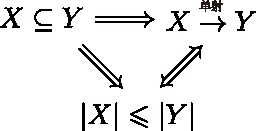
\includegraphics[width = 0.35\linewidth]{./images/implies.pdf}
\end{figure}

有限集中, 映射和基数的关系:
\begin{itemize}
    \item $ |X| < |Y| $ $ \Longleftrightarrow $ $ X \to Y $ 为单射, 但不是满射
    \item $ |X| \leqslant |Y| $ $ \Longleftrightarrow $ $ X \to Y $ 为单射
    \item $ |X| = |Y| $ $ \Longleftrightarrow $ $ X \to Y $ 为双射
\end{itemize}


\begin{proof}
    (1) 由引理 \ref{cardinary}, $ |X \cup \set{x} \setminus \set{x}| = |X| = |X \cup \set{x}| - 1 $. 所以 $ |X \cup \set{x}| = |X| + 1 $.

    (2) 设 $ |X| = n $, $ |Y| = m $. 则存在双射 $ f \colon X \to \colon \set{i \in \N \colon 1 \leqslant i \leqslant n} $ 和双射 $ g \colon Y \to \set{i \in \N \colon 1 \leqslant i \leqslant m} $. 现定义函数 $ h \colon X \cup Y \to \set{i \in \N \colon 1 \leqslant i \leqslant m + n} $.
    \[ h(x) = \begin{cases}
        f(x) & x \in X \\
        g(x) + n & x \in Y, x \notin X
    \end{cases} \]

    下面证明 $ h $ 是单射: 对于不同的 $ x, y \in X \cup Y $, 我们可以不失一般性地分类讨论三种情况. (i) 当 $ x, y \in X $: 那么 $ h(x) = f(x) $, $ h(y) = f(y) $. 由于 $ f $ 是双射, $ f(x) \neq f(y) $, 所以 $ h(x) \neq f(y) $. (ii) 当 $ x \in X $, $ y \in Y $ 且 $ y \notin X $: $ h(x) = f(x) $, $ h(y) = g(y) + n $. 由于 $ 1 \leqslant f(x) \leqslant n $, $ n + 1 \leqslant g(x) + n \leqslant n + m $, 所以有 $ h(x) \neq h(y) $. (iii) 当 $ x, y \in Y $ 且 $ x, y \notin X $: $ h(x) = g(x) + n $, $ h(y) = g(y) + n $. 而因为双射已经有 $ g(x) \neq g(y) $, 故 $ h(x) \neq h(y) $. 综上所述, $ h $ 为单射.

    当 $ X $, $ Y $ 互斥, 即 $ X \cap Y = \varnothing $. 对于每一个 $ 1 \leqslant i \leqslant n $, 能找到对应的 $ x \in X $, 满足 $ i = h(x) = f(x) $; 而对于每一个 $ n + 1 \leqslant j \leqslant m + n $, 能找到对应 $ y \in Y $, 满足 $ j = h(y) = g(y) + n $. 所以 $ h $ 是满射.

    当 $ X $, $ Y $ 不互斥, $ X \cap Y \neq \varnothing $. 考虑 $ x \in X \cap Y $, $ g(x) + n \in \set{i \in \N \colon 1 \leqslant i \leqslant m + n} $. 一方面: 对于一切 $ y \in X $, $ h(y) = f(y) $, $ 1 \leqslant f(y) \leqslant n $, $ n + 1 \leqslant g(x) + n \leqslant m + n $, 所以找不到 $ y \in X $, 满足 $ h(y) = g(x) + n $. 另一方面: 对于一切 $ y \in Y $ 但 $ y \notin X $, $ x \neq y $, $ h(y) = g(y) + n \neq g(x) + n $ (因为 $ g $ 是双射), 所以找不到 $ y \in Y $ 且 $ y \notin X $ 满足 $ h(y) = g(x) + n $. 综上所述, 找不到 $ y \in X \cup Y $, 满足 $ h(y) = g(x) + n $. 这说明 $ h $ 不是满射.

    于是综上所述, 当 $ X $, $ Y $ 互斥时, $ h \colon X \cup Y \to \set{i \in \N \colon 1 \leqslant i \leqslant m + n} $ 是双射: $ |X \cup Y| = m + n = |X| + |Y| $. 
    
    而当 $ X $, $ Y $ 不互斥时, $ h $ 仅为单射, 通过限制陪域, 构造 $ \widetilde{h} \colon X \cup Y \to h(X \cup Y) $, $ \widetilde{h} (x) = h(x) $. $ \widetilde{h} $ 是一个双射, 故 $ |X \cup Y| = |h(X \cup Y)| $. 并且 $ h(X \cup Y) \subseteq \set{i \in \N \colon 1 \leqslant i \leqslant m + n} $. 不妨记 $ H = h(X \cup Y) $, $ I = \set{i \in \N \colon 1 \leqslant i \leqslant m + n} $, $ H \subseteq I $. $ I = (I \setminus H) \cup H $, 且 $ I \setminus H $ 和 $ H $ 是互斥的. 所以 $ |I| = |I \setminus H| + |H| $, 即 $ |H| \leqslant |I| $. 所以最终, $ |X \cup Y| = |h(X \cup Y)| \leqslant |I| = m + n = |X| + |Y| $.

    (3) $ X \subseteq Y $, 则 $ Y = X \cup (Y \setminus X) $ 以及 $ X \cap (Y \setminus X) = \varnothing $. 于是由 (2) 有 $ |Y| = |X \cup (Y \setminus X)| = |X| + |Y \setminus X| \geqslant |X| $. 若 $ X \subset Y $, 存在 $ a \in Y $ 但 $ a \notin X $. 对于每一个 $ b \in X $, $ b \in Y $, $ a \neq b $. 所以 $ b \in Y \setminus \set{a} $, 所以 $ X \subseteq Y \setminus \set{a} $. 所以 $ |X| \leqslant |Y - \set{a}| = |Y| - 1 $, 则 $ |X| < |Y| $.

    (4) 单射 $ \Longrightarrow |X| \leqslant |Y| $: 反证法. 设存在单射 $ f \colon X \to Y $ 且 $ |X| > |Y| $. 那么设 $ |X| = n $, $ |Y| = m $, $ n > m $. 按照基数的定义, 存在双射 $ g \colon \set{i \in \N \colon 1 \leqslant i \leqslant n} \to X $ 以及 $ h \colon Y \to \set{i \in \N \colon 1 \leqslant i \leqslant m} $. 由命题 \ref{c}: 单射的复合仍为单射. 于是 $ h \circ f \circ g \colon \set{i \in \N \colon 1 \leqslant i \leqslant n} \to \set{i \in \N \colon 1 \leqslant i \leqslant m} $ 仍为单射. 注意到 $ \forall x \in \set{i \in \N \colon 1 \leqslant i \leqslant m} $, $ x \in \set{i \in \N \colon 1 \leqslant i \leqslant n} $, 故 $ \set{i \in \N \colon 1 \leqslant i \leqslant m} \subseteq \set{i \in \N \colon 1 \leqslant i \leqslant n} $. 由 (3): $ |\set{i \in \N \colon 1 \leqslant i \leqslant m}| \leqslant |\set{i \in \N \colon 1 \leqslant i \leqslant n}| $, 即 $ m \leqslant n $, 这与 $ n > m $ 矛盾.

    $ |X| \leqslant |Y| \Longrightarrow $ 单射: 记 $ I_{k} = \set{i \in \N \colon 1 \leqslant i \leqslant k} $. 同样设 $ |X| = n $, $ |Y| = m $, $ n \leqslant m $. 存在双射 $ f \colon X \to I_n $ 以及 $ g \colon Y \to I_m $. 可知 $ I_n \subseteq I_m $. 所以由引理 \ref{subset-injection}, 存在单射 $ h \colon I_n \to I_m $. 我们重新组织 $ f $, $ g $, $ h $ 的关系 (注意 $ Y $ 到 $ I_m $ 有双射, $ I_m $ 到 $ Y $ 也有双射): \[ X \xlongrightarrow{f} I_n \xlongrightarrow{h} I_m \xlongrightarrow{g} Y \,.\]

    那么存在 $ X $ 到 $ Y $ 的映射 $ g \circ h \circ f $, 且其为单射 (单射的复合仍为单射).

    (5) 设 $ f \colon X \to Y $, 假设 $ |f(X)| > |X| $, 那么根据 (4) 存在单射 $ g \colon X \to f(X) $, 且 $ g $ 不是满射. 这意味着存在 $ e \in f(X) $, 使得所有 $ s \in X $, 都有 $ f(s) \neq e $. 而按照像的定义 $ e \in f(X) $ 意味着存在 $ x \in X $ 满足 $ f(x) = e $, 这就产生了矛盾. 所以 $ |f(X)| \leqslant |X| $.

    而当 $ f $ 为单射. 通过限制陪域可以制造满射, 即 $ g \colon X \to f(X) $, $ g(x) = f(x) $ 是满射, 所以 $ g $ 也是双射. $ |X| \to |f(X)| $.

    (6) 设 $ X = \set{x_1, x_2, \dots, x_n} $, $ Y = \set{y_1, y_2, \dots, y_m} $. 所以有 $ |X| = n $, $ |Y| = m $. 定义 $ [n..k] \coloneqq \set{i \in \N \colon n \leqslant i \leqslant k} $, 所以 $ [1..k] $ 为 $ 1 $ 开始的 $ k $ 个整数集合. 我们构造一个函数 $ f \colon X \times Y \to [1..mn] $, $ f(x_i, y_j) = (i - 1) m + j $ , 其中 $ 1 \leqslant i \leqslant n $, $ 1 \leqslant j \leqslant m $. 为何这样选择, 思路如下:

    \begin{figure}[H]
        \centering
        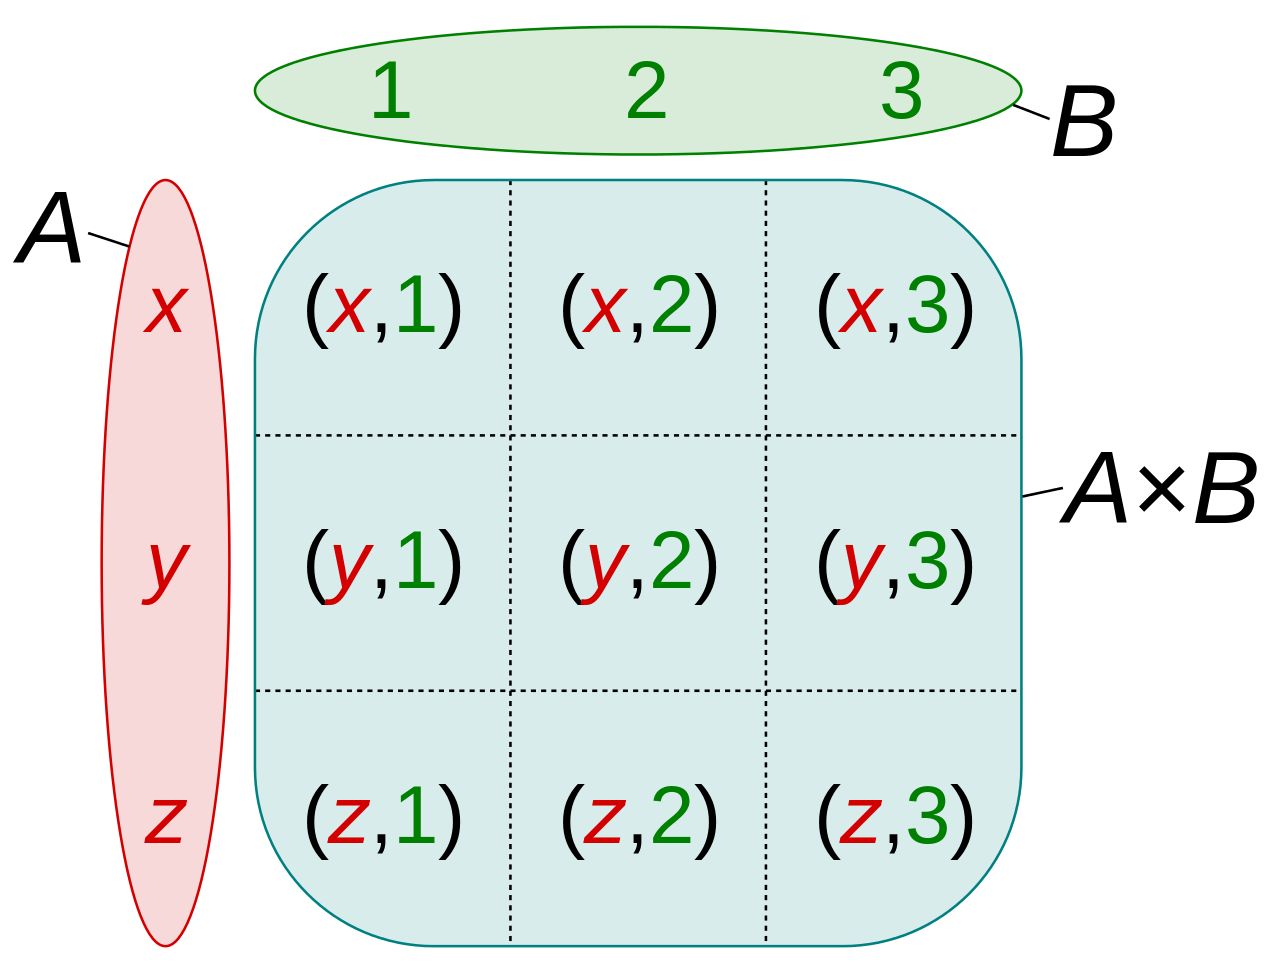
\includegraphics[width = 0.4\linewidth]{./images/Cartesian_Product.png}
    \end{figure}
    
    分别从 $ X $, $ Y $ 中选取元素, 组成了有序对, 这些有序对的集合为笛卡尔积 $ X \times Y $. 那么我们将 $ X $, $ Y $ 中的元素按行列排开, 这样笛卡尔积 $ X \times Y $ 中的元素就被排成了一个矩阵. 我们可以从左上角开始, 从左向右, 从上到下标上序号, 这样就形成了 $ X \times Y $ 中的元素到序号 $ 1, 2, \dots, n $ 的一一对应关系:
    \[     
    \begin{matrix}
         & y_1 & y_2 & \cdots & y_m \\
        x_1 & 1 & 2 & \cdots & m \\
        x_2 & m + 1 & m + 2 & \cdots & 2m \\
        \vdots & \vdots & \vdots & \ddots & \vdots \\
        x_n & n m - m + 1 & n m - m + 2 & \cdots & n m
    \end{matrix} \,,
    \]

    那么很容易得到 $ i $ 行 $ j $ 列的 $ x_i $, $ y_j $ 两元素形成的有序对 $ (x_i, y_j) $ 对应整数 $ (i - 1) m + j $. 这就是为什么 $ f $ 定义为这样. 
    
    回到证明中, 我们需要证明 $ f $ 是双射.

    \paragraph{证明 $ f $ 是单射} 
    再选两个 $ 1 \leqslant i' \leqslant n $, $ 1 \leqslant j' \leqslant m $, 需满足 $ i $ 和 $ i' $, $ j $ 和 $ j' $ 不能同时相等, 即 $ |i - i'| + |j - j'| \neq 0 $. 首先有:
    \[ i - i' \in [1 - n .. -1 ] \cup [1 .. n - 1] \,,\]
    \[ j - j' \in [1 - m .. -1 ] \cup [1 .. m - 1] \,.\]
    
    于是 $ f(x_{i'}, y_{j'}) = (i' - 1) m + j' $.
    \[ \Delta = f(x_i, y_j) - f(x_{i'}, y_{j'}) = (i - i') m + (j - j') \,.\] 
    
    若 $ i - i' = 0 $, 则 $ \Delta = 0 \cdot m + (j - j') $, 由于 $ j $, $ j' $ 不能相同, 故 $ \Delta \neq 0 $. 同理, $ j - j' = 0 $ 时, $ \Delta \neq 0 $. 那么现在考虑 $ i \neq i' $ 且 $ j \neq j' $, 假设 $ \Delta = 0 $:
    \[ m = \dfrac{j' - j}{i - i'} \,.\]

    由于 $ m $ 为正数, 分子和分母可能同正或者同负. 
    
    (i) 同正: 此时 $ 1 \leqslant j' - j \leqslant m - 1 $. 代入 $ m $:
    \[ 1 \leqslant j' - j \leqslant \dfrac{j' - j}{i - i'} - 1 \,,\]

    对于不等式的右半部分, 两边同时除以 $ j' - j $, 由于是正数, 不等号方向不变:
    \[ 1 \leqslant \dfrac{1}{i - i'} - \dfrac{1}{j' - j} \,,\]

    而此时 $ 1 \leqslant i - i' \leqslant n - 1 $, 放缩得到:
    \[ 1 \leqslant \dfrac{1}{i - i'} - \dfrac{1}{j' - j} \leqslant \dfrac{1}{1} - \dfrac{1}{j' - j} \,,\]

    而 $ \dfrac{1}{j' - j} $ 为正, 上面的不等式产生了矛盾. 故最初的假设 $ \Delta = 0 $ 错误, 应为 $ \Delta \neq 0 $.

    (ii) 对于分子分母同负的情况, 同理, 也可以得到 $ \Delta \neq 0 $.

    综上所述, 我们证明了无论何种情况, $ \Delta = f(x_i, y_j) - f(x_{i'}, y_{j'}) \neq 0 $. 即对于不同的输入, $ f $ 给出不同的输出, 所以 $ f $ 是单射.

    \paragraph{证明 $ f $ 是满射} 
    我们要证明, 对于任意的 $ t \in [1..mn] $, 总能找到 $ i \in [1..n] $, $ j \in [1..m] $, 满足 $ f(x_i, y_j) = (i - 1) m + j = t $. 我们采用归纳的思想.

    基础情形: 可以找到 $ i = n $, $ j = m $, 满足 $ (i - 1) m + j = m n $.

    现归纳地假设存在 $ t \in [1 .. mn] $, 使得存在 $ i \in [1 .. n] $, $ j \in [1 .. m] $, 满足 \[ (i - 1) m + j = t \tag{6a} \,,\] 
    
    要证明存在 $ i' \in [1 .. n] $, $ j' \in [1 .. m] $, 满足 \[ (i' - 1) m + j' = t - 1 \tag{6b} \,,\]

    将 (6a) 代入 (6b), 得到:
    \[ (i' - 1) m + j' = (i - 1) m + (j - 1) \tag{6c} \,.\]

    由于已经证明 $ f $ 是单射, 这意味着 $ (a - 1) m + b = (c - 1) m + d $ 当且仅当 $ a = c $ 且 $ b = d $. 
    
    所以对于方程 (6c), 在 $ i, i' \in [1 .. n] $ 和 $ j, j' \in [1 .. m] $ 的范围内, 可以分两种情况解得:
    \[ \begin{cases}
        i' = i \\
        j' = j - 1
    \end{cases} \quad \text{当 } 2 \leqslant j \leqslant m \,,\]
    \[ \begin{cases}
        i' = i - 1 \\
        j' = m
    \end{cases} \quad \text{当 } j = 1 \,.\]

    这说明了对于任意 $ t \in [1 .. m n] $, 都能找到 $ i \in [1 ... n] $, $ j \in [1 .. m] $, 满足 $ f(x_i, y_j) = (i - 1) m + j = t $. 即 $ f $ 为满射.

    综上所述, $ f $ 既是单射, 又是满射, 即为双射. $ f $ 是由 $ X \times Y \to [1 .. mn] $ 的双射, 所以两者有相同的基数:
    \[ |X \times Y| = |[1 .. mn]| = |\set{k \in \N \colon 1 \leqslant k \leqslant mn}| = m n = |X| |Y| \,.\]
\end{proof}


\begin{proposition}[\text{容斥原理}]
    设 $ A $, $ B $ 为有限集, 则 $ A \cup B $, $ A \cap B $ 也是有限集, 且有: $ |A \cup B| = |A| + |B| - |A \cap B| $.
\end{proposition}

\begin{proof}
    不难证得, $ A \cap B \subseteq A $, 由基数的性质 \ref{cardinal} (3), $ |A \cap B| \leqslant |A| $. 由 \ref{cardinal} (2), $ |A \cup B| \leqslant |A| + |B| $. 这两个不等式说明了, $ A \cap B $, $ A \cup B $ 为有限集.

    由命题 \ref{1.9}, $ A = (A \setminus B) \cup (A \cap B) $, $ B = (B \setminus A) \cup (A \cap B) $. 且 $ A \setminus B $, $ A \cap B $, $ B \setminus A $ 互斥. 故由 \ref{cardinal} (2):
    \[ |A| = |A \setminus B| + |A \cap B| \,,\]
    \[ |B| = |B \setminus A| + |A \cap B| \,.\]

    于是:
    \[ |A| + |B| - |A \cap B| = |A \setminus B| + |B \setminus A| + |A \cap B| \,,\]

    而由命题 \ref{1.10}: $ A \cup B = (A \setminus B) \cup (A \cap B) \cup (B \setminus A) $, 且三者互斥, 故
    \[ |A \cup B| = |A \setminus B| + |B \setminus A| + |A \cap B| \,,\]

    所以综合两个等式, 有: $ |A \cup B| = |A| + |B| - |A \cap B| $.
\end{proof}


\section{有理数和整数}
\subsection{有理数和整数}
略

\subsection{绝对值和指数运算}
略

\subsection{有理数的空隙}
\begin{proposition}[\text{有理数被整数隔开}]
    若 $ x $ 是有理数, 则存在整数 $ n $, 使得 $ n \leqslant x < n + 1 $. 特别地, 存在自然数 $ N $, 使得 $ N > x $.
\end{proposition}


\begin{proof}
    \begin{doublespace}
        (1) 当 $ x > 0 $ 时: 设 $ x = \dfrac{a}{b} $, 其中 $ a, b \in \N $. 根据欧几里得算法, 存在 $ a = b q + r $, 且 $ 0 \leqslant r < b $. 所以 $ x = \dfrac{b q + r}{b} = q + \dfrac{r}{b} $, 可见 $ q \leqslant x < q + 1 $. 下面证明唯一性, 设 $ \exists c $, $ c \leqslant x < c + 1 \Longrightarrow c \leqslant \dfrac{a}{b} < c + 1 \Longrightarrow cb \leqslant a < cb + b $. 所以 $ \exists r' $ 满足 $ a = b c + r' $. 但欧几里得算法保证了商和余数的唯一性, 即 $ c = q $, $ r' = r $.
    
        
        (2) 当 $ x < 0 $ 时: 设 $ x = -\dfrac{a}{b} $, $ a, b \in \N $. 同理有 $ a = b q + r \ (0 \leqslant r < b) $, $ x = -\left( q + \dfrac{r}{b} \right) $, 于是 $ -q - 1 < x \leqslant - q $. 于是分两种情况: 当 $ -q - 1 < x < - q $ 时, 也有 $ -q - 1 \leqslant x < -q $; 而当 $ x = -q $ 时, 有 $ -q \leqslant x < - q + 1 $. 欧几里得算法同样保证了 $ -q - 1 < x < -q $ 和 $ x = -q $ 两种情况的 $ q $ 都是唯一的, 步骤同上. 
    \end{doublespace}

    (3) 当 $ x = 0 $ 时, 显然有唯一的 $ 0 \leqslant  x < 1 $.
\end{proof}


此外, 两个有理数之间, 还有有理数. 
\begin{proposition}[\text{有理数被有理数隔开}]
    设 $ x, y $ 是任意有理数且 $ x < y $. 则 $ \exists z \in \Q $, 使得 $ x < z < y $.
\end{proposition}

\begin{proof}
    设 $ z = \dfrac{x + y}{2} $. 因为 $ x < y $, $ \dfrac{x}{2} < \dfrac{y}{2} $. 两边加上 $ y/2 $: \[ \dfrac{x}{2} + \dfrac{y}{2} < \dfrac{y}{2} + \dfrac{y}{2} \Longrightarrow z < y \,.\] 两边加上 $ x/2 $: \[ \dfrac{x}{2} + \dfrac{x}{2} < \dfrac{x}{2} + \dfrac{y}{2} \Longrightarrow x < z \,.\] 所以 $ x < z < y $.
\end{proof}

有理数的这种性质, 我们称为\textbf{稠密性}. 这说明了, 两个有理数之间还有有理数. 如果我们从数轴中切出任意小的区间, 这个区间里必然包含有理数. 但两个有理数之间任然存在无限多的空隙, 虽然稠密性保证了这些空隙无限小. 这说明有理数不是连续的, 如果对着数轴切一刀, 是有可能切不到有理数的.

比如, 对着数轴切一刀, 切出一个数 $ \sqrt{2} $ 就不是有理数.

\begin{remark}
    我们现在只定义了有理数, 不能用实数轴来理解对着数轴切一刀的概念. 可以这样想. 在有理数轴上做单位长度的线段, 在以此做一个边长为 $ 1 $ 的正方形, 按其对角线长度在数轴上切一刀 (做圆), 无法得到有理数.
\end{remark}

\begin{proposition}[\text{$ \sqrt 2 $ 不是有理数}]
    不存在 $ x \in \Q $ 使得 $ x^2 = 2 $.
\end{proposition}

\begin{proof}
    采用反证法. 设 $ x = p/q $, 其中 $ p $, $ q $ 为互质. 若 $ x^2 = 2 $, $ (p / q)^2 = 2 $. 意味着 $ p^2 = 2 q^2 $. $ p^2 = p \times p $ 为偶数, 则 $ p $ 只能为偶数. 同时 $ q^2 = p \times p / 2 $ 也为偶数, $ q $ 也只能为偶数. 这与 $ p $, $ q $ 互质矛盾. 所以不存在 $ x \in \Q $, $ x^2 = 2 $.
\end{proof}

上面的证明用到了互质和奇偶的概念.

\begin{proposition}[\text{有理数可以无限接近 $ \sqrt 2 $}]
    对于任意有理数 $ \epsilon > 0 $, 存在非负有理数 $ x $, 使得 $ x^2 < 2 < (x + \epsilon)^2 $.
\end{proposition}

\begin{proof}
    反证法. 设不存在非负的有理数, 使得 $ x^2 < 2 < (x + \epsilon)^2 $. 这等价于当 $ x^2 < 2 $ 时, $ (x + \epsilon)^2 < 2 $. 取 $ x = 0 $, $ 0^2 < 2 $, $ (0 + \epsilon)^2 < 2 $ 也成立. 因为 $ \epsilon^2 < 2 $, 又可以推出 $ (\epsilon + \epsilon)^2 < 2 $, 即 $ (2\epsilon)^2 < 2 $. 那么可以依次类推出 $ (n\epsilon)^2 < 2 $ 对每个自然数成立. 这可以根据归纳法得到证明. 于是 $ (n \epsilon)^2 < 4 \Longrightarrow n \epsilon < 2 \Longrightarrow n < \dfrac{2}{\epsilon} $ 要对一切自然数成立. 然而总能找到自然数 $ N > \dfrac{2}{\epsilon} $. 矛盾.
\end{proof}


\section{实数}
\subsection{Cauchy 序列}
\begin{definition}[\text{有理数序列}]
    序列 $ (a_n)_{n = k}^\infty $ 是 $ \set{n \in \Z \colon n \geqslant k} $ 到 $ \Q $ 的函数, 它将每一个大于等于 $ k $ 的整数都映射到一个有理数上. 由此形成了一个列有序的有理数: \[ a_{k}, a_{k + 1}, a_{k + 2}, \dots \]
\end{definition}

我们最常用的是 $ (a_n)_{n = 0}^\infty $, 即这个序列定义在 $ \N $ 上; 或是 $ (a_n)_{n = 1}^\infty $, 即定义在 $ \Z^+ $ 上. 那么下面的记号也是常用的: $ (a_n)_{n \in \N} $, $ (a_n)_{n \in \Z^+} $

\begin{remark}
    序列可以是有限的或无限的. $ (a_i)_{i = m}^n $ 就是一个有限序列: \[ a_{m}, a_{m + 1}, \dots, a_{n - 1}, a_n \]
\end{remark}

\paragraph{例}
$ (a_n)_{n \in \N} \colon a_0, a_1, a_2, \dots $

$ (a_n)_{n = 3}^\infty \colon a_3, a_4, a_5, \dots $

$ (b_n)_{n = -2}^\infty \colon b_{-2}, b_{-1}, b_0, b_1, \dots $

$ (k^2)_{k \in \N} \colon 0, 1, 4, 9, \dots $


引入一个不标准的定义帮助理解 Cauchy 序列的概念.

\begin{definition}[\text{$ \epsilon $-稳定}]
    $ (a_n)_{n \in \N} $ 是 $ \epsilon $-稳定的, 如果对于任意下标 $ i $, $ j $, 都有 $ d(a_i, a_j) \leqslant \epsilon $. 其中 $ d(x, y) \coloneqq |x - y| $, 即 $ x $ 和 $ y $ 的距离.
\end{definition}

换句话说, 序列任意两项值的距离都不大于 $ \epsilon $.

\paragraph{例}
$ (1/n)_{n = 1}^\infty \colon 1, 1/2, 1/3, \dots $ 是 $ 1 $-稳定的, 但不是 $ 0.1 $-稳定的, 因为 前两项的差为 $ 0.5 > 0.1 $.


$ \epsilon $-稳定要求序列从头到尾都符合要求, 但对于一个无限序列, 我们只需关注它的极限性状, 即下标趋于无穷时的性状, 不再关注序列的开头.

\begin{definition}[\text{终极 $ \epsilon $-稳定}]
    $ (a_n)_{n \in \N} $ 是终极 $ \epsilon $-稳定的, 当且仅当存在 $ N \geqslant 0 $, 对任意大于等于 $ N $ 的下标 $ i, j $, 有 $ d(a_i, a_j) $.
\end{definition}

也就是说: 我们不再关注 $ (a_n) $ 头几项, 而看 $ (a_n) $ 无限列下去时是不是 $ \epsilon $-稳定的.

\paragraph{例}
$ (1/n)_{n = 1}^\infty \colon 1, 1/2, 1/3, \dots $ 不是 $ 0.1 $-稳定的, 但是是终极 $ 0.1 $-稳定的. 因为从 $ n = 10 $ 开始: $ \dfrac{1}{10}, \dfrac{1}{11}, \dfrac{1}{12}, \dots $ 后面都是 $ 0.1 $-稳定的.


\begin{definition}[\text{Cauchy 序列}]
    序列 $ (a_n)_{n \in \N} $ 是柯西序列, 当且仅当对于一切有理数 $ \epsilon > 0 $, 总能找到 $ N \geqslant 0 $, 使得对任意下标 $ i, j \geqslant N $, $ d(a_i, a_j) \leqslant \epsilon $.
\end{definition}

\begin{remark}
    $ \epsilon $ 的类型不重要. 当前可以规定为有理数.
\end{remark}

\begin{remark}
    $ i, j \geqslant N $ 或是 $ i, j > N $ 无关紧要. 后面出现的定义也是一样. 同理, 最后 $ \leqslant \epsilon $ 或是 $ < \epsilon $ 也是无关紧要的. 可以证明, 这些地方使用 $ < $ 或是 $ \leqslant $ 的定义是等价的.
\end{remark}

换句话说, 对于任意小的 $ \epsilon $, $ (a_n) $ 总是终极 $ \epsilon $-稳定的: 对于任意小的 $ \epsilon $, $ (a_n) $ 在趋于无穷时总是 $ \epsilon $-稳定的.


\begin{proposition}
    序列 $ \left( \dfrac{1}{n} \right)_{n = 1}^\infty $ 是 Cauchy 序列.
\end{proposition}

\begin{proof}
    要证明该命题, 就要说明无论 $ \epsilon > 0 $ 多小, 总能找到整数正整数 $ N $, 使得当 $ i, j \geqslant N $ 时: \[ \left| \dfrac{1}{i} - \dfrac{1}{j} \right| < \epsilon \,.\]
    由于 $ i, j \geqslant N $, $ 0 < \dfrac{1}{i} < \dfrac{1}{N} $, $ 0 < \dfrac{1}{j} < \dfrac{1}{N} $, 于是 \[ \left| \dfrac{1}{i} - \dfrac{1}{j} \right| < \dfrac{1}{N} \,,\]
    令 $ \dfrac{1}{N} < \epsilon $ 即可满足条件. 此时 $ N > \dfrac{1}{\epsilon} $, 根据公理, 可以找到大于 $ \dfrac{1}{\epsilon} $ 的正整数.
\end{proof}

\begin{proposition} \label{1-1}
    序列 $ 1, -1, 1, -1, \dots $ 即 $ \big( (-1)^n \big)_{n = 0}^\infty $ 不是 Cauchy 序列. 
\end{proposition}

\begin{proof}
    假设 $ \big( (-1)^n \big)_{n = 0}^\infty $ 是 Cauchy 序列, 则对任意 $ \epsilon > 0 $, 存在 $ N \geqslant 0 $, 使得对任意 $ i, j \geqslant N $, 满足 $ \left| (-1)^i - (-1)^j \right| \leqslant \epsilon $. 不妨假设 $ j \geqslant i $, 则设 $ j = i + k $, 其中 $ k $ 为非负整数. 那么对于一切 $ k $ 和任意 $ \epsilon > 0 $, 同样应满足 $ \left| (-1)^i - (-1)^{i + k} \right| = \left| (-1)^i \big[ 1 - (-1)^k \big] \right| = \left| 1 - (-1)^k \right| \leqslant \epsilon $. 当 $ k $ 为奇数时, $ 1 - (-1)^k = 2 $, 此时对于任意 $ 0 < \epsilon < 2 $, 式子均不满足, 产生矛盾. 所以原序列不是 Cauchy 列.
\end{proof}

\begin{definition}[\text{有界序列}]
    序列 $ (a_n)_{n = k} $ 是有界的, 当且仅当存在 $ M \geqslant 0 $, 对于所有 $ i \geqslant k $, $ |a_i| \leqslant M $.
\end{definition}

\begin{proposition} \label{s}
    有限序列是有界的.
\end{proposition}

\begin{proof} \label{finite bounded}
    设 $ (a_i)_{i = 1}^n $ 是一个有界序列. 使用归纳法. $ (a_i)_{i = 1}^1 = a_1 $ 是一个有界序列, 因为 $ a_1 $ 可以以 $ |a_1| $ 为界. 现归纳地假设 $ (a_i)_{i = 1}^n $ 以 $ M $ 为界, 要证明 $ (a_i)_{i = 1}^{n + 1} $ 有界. 当 $ 1 \leqslant j \leqslant n $ 时, $ |a_j| \leqslant M \leqslant M + |a_{n+1}| $; 当 $ j = n + 1 $ 时, $ |a_j| = |a_{n+1}| \leqslant M + |a_{n+1}| $. 所以对于 $ 1 \leqslant j \leqslant n + 1 $, $ |a_j| \leqslant M + |a_{n+1}| $, $ (a_i)_{i = 1}^{n + 1} $ 以 $ M + |a_{n + 1}| $ 为界. 完成归纳. 
\end{proof}

\begin{proposition}
    每个 Cauchy 序列都是有界的.
\end{proposition}

\begin{proof}
    设 $ (a_n)_{n = 1}^\infty $ 是一个 Cauchy 序列. 那么对于任意 $ \epsilon > 0 $, 总能找到 $ N > 0 $, 当 $ i, j > N $ 时满足 $ |a_i - a_j| \leqslant \epsilon $. 那么取 $ j = N + 1 $, 也应该有 $ |a_i - a_{N+1}| \leqslant \epsilon $. 使用三角不等式 $ \big||a_i| - |a_{N+1}|\big| \leqslant |a_i - a_{N+1}| $, 所以有 $ \big||a_i| - |a_{N+1}|\big| \leqslant \epsilon \Longrightarrow  |a_i| - |a_{N+1}| \leqslant \epsilon \Longrightarrow |a_i| \leqslant \epsilon + |a_{N+1}| $. 即序列 $ (a_n)_{n = N+1}^\infty $ 以 $ \epsilon + |a_{N+1}| $ 为界. 而对于前 $ N $ 项构成的有限序列 $ (a_n)_{n = 1}^N $ 根据命题 \ref{s} 是有界的, 设其以 $ M $ 为界. 于是当 $ 1 \leqslant i \leqslant N $ 时, $ |a_i| \leqslant M \leqslant M + \epsilon + |a_{N+1}| $; 当 $ i > N $ 时, $ |a_i| \leqslant \epsilon + |a_{N+1}| \leqslant \epsilon + |a_{N+1}| + M $. 所以整个序列 $ (a_n) $ 以 $ M + \epsilon + |a_{N+1}| $ 为界.
\end{proof}


\subsection{等价的 Cauchy 序列}
\begin{definition}[\text{等价序列}]
    两个序列 $ (a_n)_{n = 1}^\infty $ 和 $ (b_n)_{n = 1}^\infty $ 等价, 当且仅当对任意小的 $ \epsilon > 0 $, 总能找到 $ N > 0 $, 使得当 $ n \geqslant N $ 时, $ d(a_n, b_n) \leqslant \epsilon $.
\end{definition}

\begin{proposition}
    序列 $ (a_n)_{n = 1}^\infty $, $ a_n = 1 + 10^{-n} $ 和 $ (b_n)_{n = 1}^\infty $, $ b_n = 1 - 10^{-n} $ 是等价的.
\end{proposition}

\begin{doublespace}
    \begin{proof}
        我们要证明对任意小的 $ \epsilon > 0 $, 总能找到 $ N > 0 $, 使得当 $ n > N $ 时, 满足 $ |a_n - b_n| = |2 \times 10^{-n}| < \epsilon $. 变换得到 $ \dfrac{2}{10^n} < \epsilon $. 通过归纳法可以证明 $ 10^n > n $ 对一切正整数成立, 于是 $ \dfrac{2}{10^n} < \dfrac{2}{n} < \epsilon $, 得到 $ n > \dfrac{2}{\epsilon} $. 所以我们可以选择大于等于 $ 2/\epsilon $ 的整数作为 $ N $, 即 $ N = \lceil {2}/{\epsilon} \rceil $.
    \end{proof}
\end{doublespace}

\begin{proposition}
    两个序列 $ (a_n)_{n = 1}^\infty $ 和 $ (b_n)_{n = 1}^\infty $ 等价. 那么 $ (a_n) $ 是 Cauchy 序列当且仅当 $ (b_n) $ 是 Cauchy 序列.
\end{proposition}

\begin{proof}
    设 $ (a_n) $ 为 Cauchy 序列. 则对于任意 $ \epsilon > 0 $, 存在 $ N_1 > 0 $, 当 $ i, j > N_1 $ 时, $ |a_i - a_j| \leqslant \epsilon $, 由于 $ \epsilon $ 是任意实数, 那么将这个实数取成 $ \epsilon/3 $ 也成立: $ |a_i - a_j| \leqslant \epsilon/3 $. 又因为 $ (a_n) $ 和 $ (b_n) $ 等价, 存在 $ N_2 > 0 $, 当 $ n > N_2 $ 时, $ |a_n - b_n| \leqslant \epsilon/3 $. 那么设 $ N = \max(N_1, N_2) $, 当 $ i, j, n > N $ 时, 上面的关系仍然成立. 现考虑任意 $ i, j > N $, $ |b_i - b_j| = |(b_i - a_i) + (a_i - a_j) + (a_j - b_j)| \leqslant |b_i - a_i| + |a_i - a_j| + |a_j - b_j| \leqslant \epsilon $. 所以 $ (b_n) $ 也是 Cauchy 序列.
\end{proof}


\subsection{实数的构造}
\begin{definition}[\text{实数}]
    实数是有理数的 Cauchy 序列的极限. 设 $ (a_n)_{n = 1}^\infty $ 是一个有理数的 Cauchy 序列, 则其极限是一个实数, 记作 $ \lim\limits_{n \to \infty} a_n $. 两个实数 $ \lim\limits_{n \to \infty} a_n $ 和 $ \lim\limits_{n \to \infty} b_n $ 是相等的, 当且仅当 $ (a_n)_{n = 1}^\infty $ 和 $ (b_n)_{n = 1}^\infty $ 是等价的.
\end{definition}

实数相等的定义是合理的: 可以证明其是自反, 对称和传递的. 此后定义的关于实数的运算, 应该满足代入公理.

\begin{remark}
    有理数 $ q $ 可以看成是实数 $ \lim\limits_{n \to \infty} q $, 即序列 $ q, q, q, \dots $ 的极限.
\end{remark}

\begin{definition}[\text{实数加法}]
    两个实数 $ a = \lim\limits_{n \to \infty} a_n $, $ b = \lim\limits_{n \to \infty} b_n $ 的加法定义为: \[ a + b \coloneqq \lim\limits_{n \to \infty} (a_n + b_n) \,.\]
\end{definition}

\paragraph{例}
$ a = \lim\limits_{n \to \infty} \left( 1 + \dfrac{1}{n} \right) $, $ b = \lim\limits_{n \to \infty} \left( 2 + \dfrac{2}{n} \right) $, 则 $ a + b = \lim\limits_{n \to \infty} \left( 1 + \dfrac{1}{n} + 2 + \dfrac{2}{n} \right) = \lim\limits_{n \to \infty} \left( 3 + \dfrac{3}{n} \right) $.

可以证明, 实数加法是良定义的. 同理, 可以定义出我们熟知的所有运算, 同样可以证明这些运算也是良定义的.

\begin{definition}[\text{实数乘法}]
    两个实数 $ a = \lim\limits_{n \to \infty} a_n $, $ b = \lim\limits_{n \to \infty} b_n $ 的乘定义为: \[ a \times b \coloneqq \lim\limits_{n \to \infty} (a_n b_n) \,.\]
\end{definition}

然后可以定义负运算, 将减法定义为加上一个负数. 所有通常的运算律, 在实数中都适用.

除法的定义稍微麻烦些. 因为不能除以 $ 0 $, 所以没法直接定义 $ a^{-1} = \lim\limits_{n \to \infty} a_n^{-1} $, 这样如果 $ a_n \to 0 $, $ a_n^{-1} $ 就发散了. 同时整个序列里不能出现 $ 0 $, 否则 $ 1/a_n $ 就会没有意义. 综上所述, 引入一个序列, 使我们能够定义除法.

\begin{definition}[\text{限制离开零的序列}]
    一个有理数的序列 $ (a_n)_{n = 1}^\infty $ 叫做是限制离开零的, 当且仅当存在一个正有理数 $ c > 0 $, 使得对于一切 $ n \geqslant 1 $, $ |a_n| \geqslant c $.
\end{definition}

\paragraph{例}
$ 1, -1, 1, -1, \dots $ 是限制离开零的, 因为所有项的绝对值都至少是 $ 1 $. 序列 $ 0.1 $, $0.01$, $0.001$, $\dots$ 不是限制离开零的. 序列 $ 0, 1, 2, 3, \dots $ 也不是限制离开零的, 因为第一项为零.


\begin{proposition}
    实数 $ x \neq 0 $, 则存在一个限制离开零的 Cauchy 序列, 其极限为 $ x $.
\end{proposition}

\begin{proposition}
    $ (a_n)_{n = 1}^\infty $ 是限制离开零的 Cauchy 序列, 则 $ (a_n^{-1}) $ 也是 Cauchy 序列.
\end{proposition}

有了限制离开零的序列, 我们可以定义倒数了:
\begin{definition}[\text{倒数}]
    设 $ x $ 是不为零的实数, $ (a_n)_{n = 1}^\infty $ 是限制离开零的有理数的 Cauchy 序列, 且 $ x = \lim\limits_{n \to \infty} a_n $. 那么定义 $ x $ 的倒数为: \[ x^{-1} \coloneqq \lim_{n \to \infty} a_n^{-1} \,.\]
\end{definition}

就此, 实数的四则运算定义完毕, 且它们满足域上所有代数运算律.


\subsection{实数的序}
实数的序的定义也要借助限制离开零的概念.

\begin{definition}[\text{正/负限制离开零}]
    称有理数列 $ (a_n)_{n = 1}^\infty $ 是正限制离开零的, 当且仅当存在一个正有理数 $ c > 0 $, 满足对 $ n > 0 $, 有 $ a_n \geqslant c $. 同理, $ (a_n)_{n = 1}^\infty $ 是负限制离开零的, 当且仅当所有的 $ a_n \leqslant -c $.
\end{definition}

也就是说, 正/负限制离开零序列的每一项都为正/负. ``正/负限制离开零'' 是比 ``限制离开零'' 更强的条件.

\paragraph{例}
$ 1.1, 1.01, 1.001, \dots $ 是限制离开零的, 也是正限制离开零的.

$ 1, -1, 1, -1, \dots $ 是限制离开零的, 但不是正/负限制离开零的.

$ -0.1, -0.01, -0.001, \dots $ 不是限制离开零的, 更不是正/负限制离开零的.

\begin{definition}[\text{实数的正负性}]
    实数 $ x $ 是正的, 如果它能写成正限制离开零的 Cauchy 序列的极限. 同理, $ x $ 是负的, 如果它能写成负限制离开零的 Cauchy 序列的极限.
\end{definition}

\begin{proposition}
    对于一个实数 $ x $, 下面三种情况恰有一种情况成立: (1) $ x $ 是正的; (2) $ x $ 是负的; (3) $ x $ 等于零.
\end{proposition}

\begin{definition}[\text{绝对值}]
    设 $ x $ 为实数. 定义 $ |x| $ 为 $ x $ 的绝对值. 当 $ x $ 为正数时, $ |x| = x $; 当 $ x $ 为负数时, $ |x| = -x $; 当 $ x = 0 $ 时, $ |x| = 0 $. 即: \[ |x| \coloneqq \begin{cases}
        x, \quad \text{当 } x \geqslant 0 \\
        -x, \quad \text{当 } x < 0
    \end{cases} \,.\]
\end{definition}

\begin{definition}[\text{实数的编序}]
    $ x $, $ y $ 为两个实数. 称 $ x $ 大于 $ y $, 如果 $ x - y $ 为正实数; 称 $ x $ 小于 $ y $, 如果 $ x - y $ 为负数. 定义大于等于 $ x \geqslant y $ 当且仅当 $ x > y $ 或 $ x = y $. 小于等于同理.
\end{definition}


\subsection{实数的确界}
\begin{definition}[\text{上界和下界}]
    对于集合 $ S \subset \R $, $ \exists M \in \R $, 使得 $ \forall s \in S $, $ s \leqslant M $, 则称 $ M $ 为 $ S $ 的\textbf{一个}上界. 同理若 $ s \geqslant m $, 则称 $ m $ 为 $ S $ 的\textbf{一个}下界.
\end{definition}

注意集合内的任意元素不大于上界, 不小于下界, 但可以取等于. 也就是说, 上下界可以是集合内的某个元素, 也可以不在这个集合中.

上界和下界是不唯一的. 但存在最小上界和最大下界, 即上确界和下确界. 集合 $ S $ 的上确界和下确界分别记为 $ \sup S $ 和 $ \inf S $.

下面以集合 $ S $ 举例, 设 $ S $ 的上界集合为 $ U $, 则最小上界 $ \beta $ 必然包含两个方面:
\begin{enumerate}
    \item $ \beta $ 是上界: $ \forall s \in S $, $ s \leqslant \beta $
    \item $ \beta $ 再小一点就不再是上界(即: 最小上界): $ \forall \epsilon > 0 $, $ \exists s \in S $, $ s > \beta - \epsilon $
\end{enumerate}

$ \beta - \epsilon $ 表示如果 $ \beta $ 再减小一点; 此时 $ \beta - \epsilon $ 就不再是上界, 意味着 $ S $ 中能够找到比 $ \beta - \epsilon $ 大的元素 $ s > \beta - \epsilon $.

上下确界满足的性质, 可以看命题 \ref{lup}.

\paragraph{例}
$ \sup\{x\in \mathbb {R} \mid 0<x<1\}=\sup\{x\in \mathbb {R} \mid 0\leq x\leq 1\} = 1 $

$ \inf\{1,2,3,\dots \}=1 $

\begin{proposition}
    任意实数 $ M $ 都是空集 $ \varnothing $ 的上界. 因为 $ M $ 大于 $ \varnothing $ 中的所有元素是一个空洞的真命题.
\end{proposition}

引入两个附加的符号 $ +\infty $ 和 $ -\infty $. 如果 $ S $ 不是空集且没有上界, 则令 $ \sup S = +\infty $; 如果 $ S = \varnothing $, 则每个实数都是空集的上界, 即 $ \sup S = -\infty $.

\begin{remark}
    $ \pm\infty $ 不是实数系 $ \R $ 的元素, 不代表一个数, 无穷代表的是一种趋近的过程. 如果希望将无穷视作一个数进行运算, 则需要将其添加到实数系中, 得到扩展后的广义实数系 $ \overline{\R} $, 并在 $ \overline \R $ 中定义关于无穷的运算, 而这有利有弊.
\end{remark}


\begin{theorem}[\text{确界存在定理}] 
    非空有上/下界的实数集必有上/下确界.
\end{theorem}

\begin{remark}
    也要注意逆否命题: 如果一个实数集没有上/下确界, 则这个实数集无界.
\end{remark}

\begin{proposition}[\text{最小上界性质(集合)}] \label{lup}
    设 $ E \subseteq \R $, $ x = \sup E $. 则:
    \begin{enumerate}
        \item 集合的每个元素不大于上确界, 即 $ x \geqslant e $ 对所有 $ e \in E $ 成立
        \item 设 $ M $ 是集合的一个上界, 则 $ M \geqslant x $
        \item 对于每一个 $ y < x $, 必然存在 $ e \in E $, 使得 $ y < e \leqslant x $, 即 $ y < e \leqslant \sup E $
    \end{enumerate}
\end{proposition}

\begin{proof}[\text{证明最小上界性质}]
    (1) 第一条即上确界的定义, 无需证明

    (2) 反证法, 设 $ M < x $. 由于 $ x $ 为上确界, 则 $ \forall \epsilon > 0 $, $ \exists e \in E $, $ x - \epsilon < e $. 现取 $ \epsilon = x - M $, $ x - \epsilon = M $. 由于 $ M $ 为上界, $ \forall e \in E $, $ M \geqslant e $, 所以有 $ x - \epsilon = M \geqslant e $ 对所有 $ e \in E $ 成立, 这与存在 $ e \in E $, $ x - \epsilon < e $ 矛盾.

    (3) 反证法. 对于每一个 $ y < x $, 假设 $ E $ 中所有 $ e $ 都有 $ e \leqslant y $ 或 $ e > x $. 由于 $ x $ 是上确界, $ e \leqslant x $, 所以只可能 $ e \leqslant y $. 而这意味着 $ y $ 是 $ E $ 的一个上界, 根据第二条性质, $ y \geqslant x $, 这与 $ y < x $ 矛盾.
\end{proof}

\begin{remark}
    上面第三条性质也可以通过确界的定义推导出来.
\end{remark}

\subsubsection{最大/最小值}
\begin{definition}
    若 $ \exists x \in S $, $ x = \sup S $, 则称 $ x $ 为 $ S $ 的最大值. 同理若 $ x = \inf S $, 则称 $ x $ 为 $ S $ 的最小值.
\end{definition}

前面提到, 上确界可以是集合的元素, 也可以不是. 当上确界是集合的元素时, 这个元素是集合的最大元素. 最小元素同理.
\paragraph{例}
$ \{ x \in \R \mid 0 < x < 1 \} $ 没有最大值, 但存在上确界为 1.

$ \{ x \in \R \mid 0 \leqslant x \leqslant 1 \} $ 有最大值 $ 1 $, 上确界 $ 1 $.


\section{序列的极限}
\subsection{收敛及极限的算律}
\begin{definition}[\text{收敛}]
    序列 $ (a_n)_{n = m}^\infty $ 收敛到 $ L $, 当且仅当对于任意实数 $ \epsilon > 0 $, 能够找到整数 $ N \geqslant m $, 使得当 $ n \geqslant N $ 时有 $ |a_n - L| \leqslant \epsilon $.
\end{definition}

\begin{remark}
    一般我们喜欢让序列从 $ 1 $ 开始, 不过从任意整数开始也可以. 事实上, 序列从哪里起始我们并不关心, 我们关注的是数列的极限, 即趋于无穷时的性质.
\end{remark}

换句话说, 给定任意小的 $ \epsilon $, 总能找到数列的某一项, 这一项之后的每一项和 $ L $ 的距离都小于等于给定的 $ \epsilon $. 也即: 无论 $ \epsilon $ 取得多小, 序列和 $ L $ 的距离最终都会小于 $ \epsilon $.

\begin{proposition}
    序列 $ 0.9, 0.99, 0.999, \dots $ 收敛于 $ 1 $.
\end{proposition}

\begin{proof}
    这个序列为 $ (1 - 10^{-n})_{n = 1}^\infty $, 要证明这个命题, 就要证明对于一切 $ \epsilon > 0 $, 存在 $ N \geqslant 1 $, 当 $ n > N $ 时, 恒有 $ |a_n - 1| = |1 - 10^{-n} - 1| \leqslant \epsilon $. 即 $ 10^{-n} \leqslant \epsilon $. 将 $ 10^{-n} $ 放大, 因为 $ 10^{-n} < 1/n $ 对于一切正整数成立. 故有 $ 10^{-n} < 1/n \leqslant \epsilon \Longrightarrow n \geqslant 1/\epsilon $. 所以取 $ N = \lceil 1/\epsilon \rceil $, 就找到了满足条件的 $ N $. 
\end{proof}

这个命题说明了 $ 0.999\cdots = 1 $.

\begin{proposition}[\text{极限的唯一性}]
    设 $ L $ 和 $ L' $ 是两个不同的实数. 则序列 $ (a_n)_{n = m}^\infty $ 不可能同时收敛到 $ L $ 和 $ L' $.
\end{proposition}

\begin{proof}
    假设 $ (a_n)_{n = m}^\infty $ 同时收敛到不同的 $ L $ 和 $ L' $. 那么对于任意正实数 $ \epsilon $, 我们总可以找到充分大的 $ N $, 使得当 $ n > N $ 时, 既有 $ |a_n - L| \leqslant \epsilon $ 且 $ |a_n - L'| \leqslant \epsilon $. $ L \neq L' $, $ |L - L'| > 0 $. 取 $ \epsilon = |L - L'| / 3 $, 于是 $ |a_n - L| + |a_n - L'| \leqslant 2 |L - L'|/3 $, 根据三角不等式, $ |L - L'|\leqslant |a_n - L| + |a_n - L'| \leqslant 2 |L - L'|/3 $, 所以 $ |L - L'| \leqslant 2 |L - L'|/3 \Longrightarrow |L - L'| = 0 $, 这与 $ |L - L'| > 0 $ 矛盾.
\end{proof}


\begin{definition}[\text{序列的极限}]
    若序列 $ (a_n)_{n = m}^\infty $ 收敛到 $ L $, 则称该序列的极限为 $ L $, 记作 $ \lim\limits_{n \to \infty} a_n = L $; 或者称 $ n \to \infty $ 时, $ a_n \to L $. 若 $ (a_n)_{n = m}^\infty $ 不收敛到任何实数, 则称该序列发散.
\end{definition}

\begin{remark}
    序列 $ (a_n)_{n = m}^\infty $ 发散. 可以称 $ \lim\limits_{n \to \infty} a_n $ 无定义或不存在 (DNE), 记作 $ \lim\limits_{n \to \infty} a_n = \text{DNE} $; 也可以称该序列发散到无穷, 记作 $ \lim\limits_{n \to \infty} a_n = \infty $. 如果是广义实数系, 我们也可以说其收敛到无穷, 不过目前暂且不考虑这种说法.
\end{remark}

\begin{proposition}[\text{收敛的序列是 Cauchy 列}] \label{convergent}
    若 $ (a_n)_{n = m}^\infty $ 是一个收敛的实数列, 则 $ (a_n) $ 是一个 Cauchy 列.
\end{proposition}

\begin{proof}
    设 $ (a_n)_{n = m}^\infty $ 是一个收敛于 $ L $ 的实数列. 则对于任意实数 $ \epsilon > 0 $, 存在 $ N \geqslant m $, 使得 $ i > N $ 时有, $ |a_i - L| \leqslant \epsilon $. 既然 $ \epsilon $ 为任意整数, 不妨����� $ |a_i - L| \leqslant \epsilon/2 $. 于是可以做变换 $ |a_i - a_j + a_j - L| \leqslant \epsilon/2 $. 其中下标 $ j > N $. 根据三角不等式, $ |a_i - a_j + a_j - L| \geqslant \big| |a_i - a_j| + |a_j - L| \big| $. 所以有 $ \big| |a_i - a_j| + |a_j - L| \big| \leqslant \epsilon /2 \Longrightarrow |a_i - a_j| + |a_j - L| \leqslant \epsilon / 2 \Longrightarrow |a_i - a_j| \leqslant \epsilon/2 + |a_j - L| $, 而 $ |a_j - L| \leqslant \epsilon/2 $, 所以 $ |a_i - a_j| \leqslant \epsilon $. 即 $ (a_n)_{n = m}^\infty $ 为 Cauchy 列.
\end{proof}

同样实数列可以定义有界的概念, 这与有理数列的有界是相容的. 

\begin{proposition}[\text{极限的算律}]
    设 $ (a_n)_{n = m}^\infty $ 和 $ (b_n)_{n = m}^\infty $ 为收敛的序列, 即 $ \displaystyle \lim_{n \to \infty} a_n $ 和 $ \displaystyle \lim_{n \to \infty} b_n $ 都为实数. 则有下面的关系:
    \begin{enumerate}
        \item (可加性) $ \displaystyle \lim_{n \to \infty} (a_n + b_n) = \lim_{n \to \infty} a_n + \lim_{n \to \infty} b_n $
        \item (一次齐次) $ \displaystyle \lim_{n \to \infty} (c a_n) = c \lim_{n \to \infty} a_n $
        \item (乘法) $ \displaystyle \lim_{n \to \infty} (a_n b_n) = \lim_{n \to \infty} a_n \cdot \lim_{n \to \infty} b_n $
        \item (倒数) 当 $ \displaystyle \lim_{n \to \infty} a_n \neq 0 $ 时: $ \displaystyle \lim_{n \to \infty} a_n^{-1} = \left( \lim_{n \to \infty} a_n \right)^{-1} $
        \item (除法) 当 $ \displaystyle \lim_{n \to \infty} b_n \neq 0 $ 时: $ \displaystyle \lim_{n \to \infty} \dfrac{a_n}{b_n} = \dfrac{\lim_{n \to \infty} a_n}{\lim_{n \to \infty} b_n} $
        \item (最大值函数)  $ \displaystyle \lim_{n \to \infty} \max (a_n, b_n) = \max (\lim_{n \to \infty} a_n, \lim_{n \to \infty} b_n) $
        \item (最小值函数)  $ \displaystyle \lim_{n \to \infty} \min (a_n, b_n) = \min (\lim_{n \to \infty} a_n, \lim_{n \to \infty} b_n) $
    \end{enumerate}
\end{proposition}

\begin{remark}
    1, 2 两条说明极限是线性运算.
\end{remark}

\begin{corollary}
    $ \displaystyle \lim_{n \to \infty} |a_n| = \left| \lim_{n \to \infty} a_n \right| $.
\end{corollary}

可以将绝对值定义为 $ |x| \coloneqq \max (x, -x) $, 这样应用上面的极限算律可以很容易证明该推论.


\subsection{广义实数系}
将 $ \pm \infty $ 加入到实数系 $ \R $ 中, 得到广义实数系: \[ \overline \R = \R \cup \set{+\infty, -\infty} \,.\]

对 $ x \in \overline \R $, 如果 $ x \in \R $, 则称 $ x $ 是有限的; 如果 $ x = +\infty $ 或 $ x = -\infty $, 则称 $ x $ 是无穷的. 对于这个数系, 我们只定义负运算和序. 引入加法、乘法等运算会带来麻烦, 故不做此工作:

将 $ \R $ 上的负运算 $ x \mapsto -x $ 拓广到 $ \overline \R $ 中, 定义: $ -(+\infty) = -\infty $, $ -(-\infty) = +\infty $. 于是对于任意 $ x \in \overline \R $, $ -(-x) = x $.

定义 $ \overline \R $ 上的序. 称广义实数 $ x \leqslant y $, 当且仅当下面三个命题之一成立:
\begin{itemize}
    \item $ x $, $ y $ 为实数, 且 $ x \leqslant y $
    \item $ y = +\infty $
    \item $ x = -\infty $
\end{itemize}

称 $ x < y $ 当且仅当 $ x \leqslant y $ 且 $ x \neq y $.

还可以定义确界, 设 $ E \subseteq \R $, 则可以定义上确界 $ \sup E $ 为:
\begin{itemize}
    \item 若 $ E \subseteq \R $, 则按之前的定义 $ \sup E $
    \item 若 $ E $ 包含 $ +\infty $, 则 $ \sup E = +\infty $
    \item 若 $ E $ 不包含 $ +\infty $ 但包含 $ -\infty $, 则 $ \sup E = \sup (E \setminus \set{-\infty}) $ (落入第一种情况)
\end{itemize}

可以定义下界: $ \inf E = - \sup (-E) $.



\subsection{序列的确界}
序列也可定义确界的概念: 将序列的每一项放入一个集合, 考虑这个集合的确界即可.

\begin{definition}
    序列 $ (a_n)_{n = m}^\infty $ 是一个实数列, 则可定义其上确界: \[ \sup (a_n)_{n = m}^\infty \coloneqq \sup \set{a_n \colon n \geqslant m} \,.\] 同理可以定义下确界: \[ \inf (a_n)_{n = m}^\infty \coloneqq \inf \set{a_n \colon n \geqslant m} \,.\]
\end{definition}

\begin{remark}
    $ \sup (a_n)_{n = m}^\infty $ 也可以写成 $ \sup\limits_{n \geqslant m} a_n $, 这里两种形式的 $ n $ 都是下标, 选取哪个字母无关紧要, 所以也称哑元 (dummy index). 如: $ \displaystyle \sup_{n \geqslant m} a_n $ 和 $ \displaystyle \sup_{k \geqslant m} a_k $ 意思一样.
\end{remark}

\paragraph{例}
$ (a_n)_{n = 1}^\infty \colon 1, -1, 1, -1, \dots $ 将每一项放入集合 $ \set{a_n \colon n \geqslant 1} = \set{1, -1} $, 所以 $ (a_n)_{n = 1}^\infty $ 的上确界为 $ \sup\set{1, -1} = 1 $.

\paragraph{例}
$ (1/n)_{n = 1}^\infty $ 的下确界为 $ \inf (a_n)_{n = 1}^\infty = \inf\set{1, 1/2, 1/3, \dots} = 0 $, 上确界为 $ \sup\limits_{n > 0} a_n = \sup\set{1, 1/2, 1/3, \dots} = 1 $.


\begin{proposition}[\text{最小上界性质(序列)}]
    设序列 $ (a_n)_{n = m}^\infty $ 的最小上界为 $ x = \sup\limits_{n \geqslant m} a_n $. 则
    \begin{enumerate}
        \item 序列的每一项不大于上确界, 即 $ a_n \leqslant x $ 对所有 $ n \geqslant m $ 成立
        \item 设 $ M $ 是序列的一个上界, 则 $ M \geqslant x $
        \item 对于每一个 $ y < x $, 必然存在 $ n \geqslant m $, 使得 $ y < a_n \leqslant x $, 即 $ y < a_n \leqslant \sup\limits_{n \geqslant m} a_n $
    \end{enumerate}
\end{proposition}

(无限)序列的确界本质就是无限集合的确界. 所以对应的可以有集合确界的最小上界性质. 同理还有最大下界性质, 这里再次引用.

\paragraph{最小上界性质(集合)}
    设 $ E \subseteq \R $, $ x = \sup E $. 则:
    \begin{enumerate}
        \item 集合的每个元素不大于上确界, 即 $ x \geqslant e $ 对所有 $ e \in E $ 成立
        \item 设 $ M $ 是集合的一个上界, 则 $ M \geqslant x $
        \item 对于每一个 $ y < x $, 必然存在 $ e \in E $, 使得 $ y < e \leqslant x $, 即 $ y < e \leqslant \sup E $
    \end{enumerate}


序列的确界性质也可以照着集合的确界性质证明, 只需做微小改动.


\begin{theorem}[\text{单调收敛定理}] \label{monotone convergence}
    设实数序列 $ (a_n)_{n = m}^\infty $ 为一个递增的序列, 即 $ a_{n+1} \geqslant a_n $. 若该序列有上界 $ M $, 则这个序列必然收敛, 且收敛到上确界 \[ \lim\limits_{n \to \infty} a_n = \sup\limits_{n \geqslant m} a_n \leqslant M \,.\]
\end{theorem}

同理, 递减有下界的序列也收敛.

\begin{proof}
    设递增序列 $ (a_n)_{n = m}^\infty $ 的上确界为 $ x = \sup_{k \geqslant m} a_k $. 根据上确界的定义, $ x \geqslant a_n $ 对于所有 $ n \geqslant m $ 成立. 要证 $ (a_n)_{n = m}^\infty $ 收敛到 $ x = \sup_{k \geqslant m} a_k $, 即要证对于任意 $ \epsilon > 0 $, 存在 $ N \geqslant m $, 使得 $ n \geqslant N $ 时, $ |a_n - x| \leqslant \epsilon $. 而 $ x \geqslant a_n $, 要证的不等式化简为 $ x - a_n \leqslant \epsilon \Longleftrightarrow  a_n \geqslant x - \epsilon $. 再次根据上确界的定义, 对于任意 $ \epsilon > 0 $, 存在 $ n \geqslant m $ 使得 $ a_n > x - \epsilon $. 设 $ a_{N'} > x - \epsilon $. 由于序列递增 $ a_{n + 1} \geqslant a_n $ 对任意的 $ n \geqslant m $ 成立, 则 $ a_{n + 1} \geqslant a_n > x - \epsilon $. 于是通过归纳法, 可以得到 $ a_n > x - \epsilon $ 对于所有的 $ n \geqslant N' $ 成立. 而这证明了: 存在 $ N \geqslant m $, 使得 $ n \geqslant N $ 时, $ a_n > x - \epsilon $ 即 $ |a_n - x| \leqslant \epsilon $.
\end{proof}


\subsection{上极限和下极限}
序列 $ a_n \colon 1.1, 1.01, 1.001, \dots $ 的极限为 $ 1 $; 序列 $ b_n \colon -1.1, -1.01, -1.001, \dots $ 的极限为 $ -1 $. 但当我们把两个序列混合起来: $ a_1, b_1, a_2, b_2, \dots $, 这个序列就不再有极限. 但是 $ 1 $ 和 $ -1 $ 和这个混合序列似乎仍然存在着一种关系. 这就要引入上极限和下极限.

\begin{definition}[\text{极限点}]
    实数 $ x $ 是 $ (a_n)_{n = m}^{\infty} $ 的极限点, 当且仅当对于任意实数 $ \epsilon > 0 $, 和每一个 $ N \geqslant m $, 都存在至少一个 $ n \geqslant N $, 满足 $ d(a_n, x) \leqslant \epsilon $. 
\end{definition}

\begin{remark}
    注意极限点和极限的区别. 它们的定义存在微妙的量的差别.

    极限: $ \forall \epsilon > 0 $, $ \exists N \geqslant m $, $ \forall n \geqslant N $, $ d(a_n, L) \leqslant \epsilon $.

    极限点: $ \forall \epsilon > 0 $, $ \forall N \geqslant m $, $ \exists n \geqslant N $, $ d(a_n, x) \leqslant \epsilon $.

    含义上, 我们只关注序列趋于无穷时的 ``极限性状'', 而忽略序列开头的任意有限项:

    极限: 无论 $ \epsilon $ 有多小, 这个序列 ``趋于无穷时的每一项'' 都会和 $ x $ 距离小于 $ \epsilon $.

    极限点: 无论 $ \epsilon $ 有多小, 这个序列趋于无穷时, 至少部分项会和 $ x $ 距离小于 $ \epsilon $.

    因此可以看出, 极限是极限点的特殊情况 (极限强于极限点). 
\end{remark}

\begin{proposition}[\text{极限是极限点}]
    $ (a_n)_{n = m}^\infty $ 收敛到 $ L $, 则 $ L $ 是其唯一的极限点.
\end{proposition}


整个过程可以这样想: 从第一项开始看, 看从这一项开始能不能找到满足条件的 $ x $: $ a_1, a_2, a_3, \dots $ 里面可以找到一个 $ a_n $ 满足 $ a_n $ 和 $ x $ 的距离不大于 $ \epsilon $. 现在从第二项开始找, $ a_2, a_3, \dots $ 里面也能找到满足条件的项. 继续从第三项, 第四项开始. 无论从哪一项开始, 往后总能找到至少一个项, 满足这个项和 $ x $ 的距离小于任意给定的 $ \epsilon $, 所以 $ x $ 就是极限点.


\paragraph{例}
序列 $ 0.9, 0.99, 0.999, \dots $. 无论从哪一项开始, 这一项之后总能找到至少一项, 使得这一项和 $ 1 $ 的距离小于给定的任意小的 $ \epsilon $, 所以极限点为 $ 1 $. 而 $ 0.8 $ 不是极限点, 因为若取 $ \epsilon = 0.1 $, 从第二项开始看, $ a_2, a_3, a_4, \dots $ 中找不到一项, 满足和 $ 0.8 $ 的距离小于等于 $ 0.1 $.

\paragraph{例}
序列 $ 1.1, -1.1, 1.01, -1.01, 1.001, -1.001, \dots $ 有两个极限点 $ 1 $ 和 $ -1 $.

\paragraph{例}
序列 $ 1, 0, -1, 0, 1, 0, -1, \dots $ 有三个极限点 $ 1 $, $ 0 $ 和 $ -1 $.


考察两个特殊的极限点: 上极限和下极限.
\begin{definition}[\text{上/下极限}]
    设序列 $ (a_n)_{n = m}^\infty $, 序列从第 $ N $ 项开始往后的序列的上界为 $ \sup\limits_{n \geqslant N} a_n $, 而 $ N $ 从第一项开始往后取, $ m, m + 1, \dots $, 构成了一个关于上确界的序列 $ \Big( \sup\limits_{n \geqslant N} a_n \Big)_{N = m}^\infty $, 这个序列的下确界, 就是原序列的上极限, 即: \[ \limsup_{n \to \infty} a_n \coloneqq \inf_{N \geqslant m} \sup_{n \geqslant N} a_n  \,.\] 上极限的等价定义是, 当 $ N \to \infty $ 时, 上确界序列的极限就是序列的上极限: \[ \limsup_{n \to \infty} a_n \coloneqq \lim_{N \to \infty} \sup_{n \geqslant N} a_n \,.\] 同理可以定义下极限: \[ \liminf_{n \to \infty} a_n \coloneqq \sup_{N \geqslant m} \inf_{n \geqslant N} a_n \,,\] \[ \liminf_{n \to \infty} a_n \coloneqq \lim_{N \to \infty} \inf_{n \geqslant N} a_n \,.\] 
\end{definition}


\paragraph{例}
序列 $ (a_n)_{n = 1}^\infty \colon 1.1, -1.1, 1.01, -1.01, 1.001, -1.001, \dots $

设从第 $ N $ 项开始的序列上确界为 $ a_N^+ = \sup\limits_{n \geqslant N} a_n $. 则序列 $ a_1^+, a_2^+, \dots $ 为 $ 1.1 $, $1.01$, $1.001$, $\dots $, 这个序列的下确界为 $ 1 $, 所以 $ (a_n)_{n = 1}^\infty $ 的上极限为 $ 1 $.

同理定义从第 $ N $ 项开始的序列的下确界为 $ a_N^- = \inf\limits_{n \geqslant N} a_n $. 则序列 $ a_1^-, a_2^-, \dots $ 为 $ -1.1, -1.01, -1.001, \dots $, 这个序列的上确界为 $ -1 $, 故 $ (a_n)_{n = 1}^\infty $ 的下极限为 $ -1 $.

\paragraph{例}
$ 1, -2, 3, -4, 5, \dots $ 的上极限是 $ +\infty $, 下极限是 $ -\infty $.

$ 1, 2, 3, 4, 5, \dots $ 的上极限是 $ +\infty $, 下极限是 $ +\infty $.

% \begin{proof}[\text{证明两种定义方式等价}]
%     以上极限为例, 证明: $\displaystyle \inf_{N \geqslant m} \sup_{n \geqslant N} a_n \equiv \lim_{N \to \infty} \sup_{n \geqslant N} a_n $.
% \end{proof}


\begin{proposition}[\text{上下极限性质}] \label{limsup}
    设 $ (a_n)_{n = m}^\infty $ 是实数序列. $ L^+ $, $ L^- $ 分别是序列的上极限和下极限, 且 $ L^+, L^- $ 是广义实数.
    \begin{enumerate}
        \item 对每一个 $ x > L^+ $, 存在 $ N \geqslant m $, 当 $ n \geqslant N $ 时, $ a_n < x $. ($ a_n $ 最终会小于 $ x $) 同理, 对 $ x < L^- $ 有类似的 $ a_n > x $
        \item 对每一个 $ x < L^+ $, 对所有 $ N \geqslant m $, 总能找到至少一个 $ n \geqslant N $, 满足 $ a_n > x $. ($ a_n $ 无限次超过 $ x $) 同理, 对 $ x > L^- $ 有类似的 $ a_n < x $
        \item $ \inf\limits_{n \geqslant m} a_n \leqslant L^- \leqslant L^+ \leqslant \sup\limits_{n \geqslant m} a_n $
        \item $ c $ 是 $ (a_n)_{n = m}^\infty $ 的极限点, 则 $ L^- \leqslant c \leqslant L^+ $
        \item 若 $ L^+ $ (或 $ L^- $) 有限, 则 $ L^+ $ (或 $ L^- $) 是 $ (a_n)_{n = m}^\infty $ 的极限点
        \item 设 $ c $ 为实数. $ (a_n)_{n = m}^\infty $ 收敛到 $ c $ 当且仅当 $ L^- = L^+ = c $.
    \end{enumerate}
\end{proposition}

\begin{remark}
    上极限是最大的极限点, 下极限是最小的极限点. 上下极限重合, 则序列收敛, 这个唯一的极限点就成为序列的极限.
\end{remark}

\begin{proof}
    (1) 利用确界性质, 从外向内去掉 $ \inf $ 和 $ \sup $. 
    
    已知 $ x > L^+ = \inf \Big( \sup (a_n)_{n = N}^\infty \Big)_{N = m}^\infty $. 根据最大下界性质, 存在 $ N \geqslant m $, $ x > \sup(a_n)_{n = N}^\infty \geqslant \inf \Big( \sup (a_n)_{n = N}^\infty \Big)_{N = m}^\infty $, 即 $ x > \sup (a_n)_{n = N}^\infty $. 根据最小上界性质, $ x > \sup (a_n)_{n = N}^\infty \geqslant a_n $ 即 $ x > a_n $ 对于所有 $ n \geqslant N $ 成立.

    (2) 思路同 (1). 根据确界原理, 对于一切 $ N \geqslant m $, 有 $ \displaystyle x < L^+ = \inf_{N \geqslant m} \sup_{n \geqslant N} a_n \leqslant \sup_{n \geqslant m} a_n $. 即有 $\displaystyle x < \sup_{n \geqslant m} a_n $, 则根据确界性质, 存在 $ n \geqslant m $, $\displaystyle x < a_n \leqslant \sup_{n \geqslant m} a_n $ 对所有 $ N \geqslant m $ 成立.

    (3) I. 证明 $ \sup\limits_{n \geqslant m} a_n \geqslant L^+ $: 根据确界性质, $ L^+ = \inf\limits_{N \geqslant m} \sup\limits_{n \geqslant N} a_n \leqslant \sup\limits_{n \geqslant N} a_n $ 对一切 $ N \geqslant m $ 成立. $ \displaystyle L^+ \leqslant \sup_{n \geqslant N} a_n $ 中取 $ N = m $ 即可.

    II. 证明 $ \displaystyle L^- \geqslant \inf_{n \geqslant m} a_n $: 根据确界性质, $ \displaystyle L^- = \sup_{N \geqslant m} \inf_{n \geqslant N} a_n \geqslant \inf_{n \geqslant N} a_n $ 对一切 $ N \geqslant m $ 成立. $ \displaystyle L^- \geqslant \inf_{n \geqslant N} $ 中取 $ N = m $ 即可.

    III. 证明 $ L^+ \geqslant L^- $: 假设 $ L^+ < L^- $, 则可以取 $ L^+ < M < L^- $. 根据 (1) 中命题, $ L^+ < M $, 则存在 $ N_1 \geqslant m $, 当 $ n \geqslant N_1 $ 时, $ a_n < M $. 同理 $ L^- > M $, 存在 $ N_2 \geqslant m $, 当 $ n \geqslant N_2 $ 时, $ a_n > M $. 则存在 $ N = \max (N_1, N_2) $, 当 $ n > N $ 时, 同时有 $ a_n < M $ 和 $ a_n > M $, 矛盾. 故不可能 $ L^+ < L^- $, 所以 $ L^+ \geqslant L^- $.

    (4) 反证法, 假设 $ c $ 是 $ (a_n)_{n = m}^\infty $ 的极限点, 且 $ c > L^+ $ 或 $ c < L^- $. 我们要从两种情况中推出矛盾. 
    
    首先看 $ c > L^+ $, 由 (1), $ \exists N_1 \geqslant m $, 当 $ n > N_1 $, $ c > a_n $. $ c $ 是极限点, 则 $ \forall \epsilon > 0 $, $ \forall N \geqslant m $, $ \exists n > N $, $ |a_n - c| \leqslant \epsilon $. 那么当 $ n > N_1 $, $ \epsilon $ 取 $ c - L^+ $ 时, 也应该有上面的不等式, 而 $ c > a_n $, $ |a_n - c| = c - a_n \leqslant \epsilon = c - L^+ \Longrightarrow L^+ \leqslant a_n \Longrightarrow L^+ \leqslant a_n \leqslant \sup\limits_{n \geqslant m} a_n $, 而这与 (3) 中结论 $ \displaystyle \sup_{n \geqslant m} a_n \geqslant L^+ $ 矛盾. 
    
    同理, 再假设 $ c < L^- $. 由 (1), $ \exists N_2 \geqslant m $, 当 $ n > N_2 $, $ c < a_n $. $ c $ 是极限点, 则 $ \forall \epsilon > 0 $, $ \forall N \geqslant m $, $ \exists n > N $, $ |a_n - c| \leqslant \epsilon $. 那么当 $ n > N_2 $, $ \epsilon $ 取 $ L^- - c $ 时, 也应该有上面的不等式, 而 $ a_n > c $, $ |a_n - c| = a_n - c \leqslant \epsilon = L^- - c \Longrightarrow L^- \geqslant a_n \Longrightarrow a_n \geqslant L^- \geqslant \inf\limits_{n \geqslant m} a_n $, 而这与 (3) 中结论 $ \displaystyle \inf_{n \geqslant m} a_n \leqslant L^- $ 矛盾. 

    (5) 设 $ x = L^+ + \epsilon $, 其中 $ \epsilon $ 为任意正数. 则 $ x > L^+ $, 应用 (1), 存在 $ N_1 \geqslant m $, 当 $ n \geqslant N_1 $ 时, $ x > a_n $. 而这蕴含: 对于所有 $ N_1 \geqslant m $, 存在 $ n \geqslant N_1 $, $ x > a_n $. 
    
    同理, 设 $ y = L^+ - \epsilon $, 则 $ y < L^+ $, 应用 (2), 对于一切 $ N_2 \geqslant m $, 存在 $ n \geqslant N_2 $, 使得 $ y < a_n $. 
    
    综上所述, 对于任意 $ N \geqslant m $, 存在 $ n \geqslant N $, 满足 $ y < a_n < x $ 即 $ L^+ - \epsilon < a_n < L^+ + \epsilon $ 也即 $ |a_n - L^+| < \epsilon $. 而这对任意 $ \epsilon > 0 $ 均成立, 故证明了 $ L^+ $ 是一个极限点.

    (6) \paragraph{正推} 若 $ (a_n)_{n = m}^\infty $ 收敛到 $ c $, 证明 $ L^- = L^+ = c $. 
    
    假设 $ L^- \neq L^+ $. 根据 (3), $ L^- < L^+ $. 根据 (4), $ c $ 一定在 $ L^- $ 和 $ L^+ $ 之间. 故有: $ L^- \leqslant c \leqslant L^+ $, 且不能同时取等. 那么 $ L^- < c $ 或 $ c < L^+ $ 至少有一个成立. 首先根据 (3), 有 $ \inf\limits_{n \geqslant m} a_n \leqslant L^- \leqslant L^+ \leqslant \sup\limits_{n \geqslant m} a_n $, 若 $ L^- $ 和 $ L^+ $ 是无限的, 则 $ \displaystyle \inf_{n \geqslant m} a_n $ 和 $ \displaystyle \sup_{n \geqslant m} a_n $ 也是无限的, 这意味着 $ (a_n)_{n = m}^\infty $ 无上下确界, 也就无界, 这和序列收敛矛盾. 故 $ L^- $ 和 $ L^+ $ 一定有限. 

    I. 对于 $ L^- < c $, 根据 (5), $ L^- $ 是 $ (a_n)_{n = m}^\infty $ 的极限点, 所以 $ \forall \epsilon > 0 $, $ \forall N \geqslant m $, $ \exists n > N $, $ |a_n - L^-| \leqslant \epsilon / 2 $. 又因为序列收敛到 $ c $, 所以 $ \forall \epsilon > 0 $, $ \exists N_1 \geqslant m $, $ \forall n > N_1 $, $ |a_n - c| \leqslant \epsilon / 2 $. 于是存在 $ n > N_1 $, 同时满足 $ |a_n - L^-| \leqslant \epsilon / 2 $ 和 $ |a_n - c| \leqslant \epsilon / 2 $. 所以有 $ |a_n - L^-| + |a_n - c| \leqslant \epsilon / 2 + \epsilon / 2 $. 根据三角不等式, $ |a_n - L^-| + |a_n - c| \geqslant |c - L^-| $, 故 $ |c - L^-| \leqslant \epsilon $. $ c > L^- $, 取 $ \epsilon = \dfrac{c - L^-}{2} $, 代入上式得到 $ c - L^- \leqslant (c - L^-)/2 $ 即 $ c \leqslant L^- $, 这与 $ L^- < c $ 矛盾.

    II. 对于 $ c < L^+ $, 同理, 存在 $ n > N_2 $, 同时满足 $ |a_n - L^+| < \epsilon / 2 $ 和 $ |a_n - c| \leqslant \epsilon / 2 $. 相加得到并应用三角不等式 $ |c - L^+| \leqslant \epsilon $. 由于 $ c < L^+ $, 取 $ \epsilon = (L^+ - c) / 2 $, 代入上式化简得到, $ L^+ \leqslant c $, 这与 $ c < L^+ $ 矛盾.

    所以 $ L^- \neq L^+ $ 的假设错误, $ L^- = L^+ $. 根据 (4), $ L^- \leqslant x \leqslant L^+ $, 所以 $ L^- = L^+ = c $.

    \paragraph{反推}
    若 $ L^- = L^+ = c $, 要证明 $ (a_n)_{n = m}^\infty $ 收敛到 $ c $.

    设 $ \epsilon > 0 $ 为任意正实数. $ c + \epsilon > L^+ $, 由 (1), 存在 $ N_1 \geqslant m $, $ n > N_1 $, $ a_n < c + \epsilon $. 同理 $ c - \epsilon < L^- $, 由 (1), 存在 $ N_2 \geqslant m $, $ n \geqslant N_2 $, $ c - \epsilon < a_n $. 于是, 对于任意 $ \epsilon > 0 $, 存在 $ N = \max (N_1, N_2) $, 当 $ n > N $ 时, $ c - \epsilon < a_n < c + \epsilon $, 即 $ |a_n - c| < \epsilon $.
\end{proof}

\begin{lemma}[\text{比较原理}]
    设 $ (a_n)_{n = m}^\infty $, $ (b_n)_{n = m}^\infty $ 是两个实数列. 且 $ (a_n) $ 的每一项都小于等于 $ (b_n) $, 即对所有 $ n \geqslant m $, $ a_n \leqslant b_n $, 则:
    \[ \sup_{n \geqslant m} a_n \leqslant \sup_{n \geqslant m} b_n \,,\]
    \[ \inf_{n \geqslant m} a_n \leqslant \inf_{n \geqslant m} b_n \,,\]
    \[ \limsup_{n \to \infty} a_n \leqslant \limsup_{n \to \infty} b_n \,,\]
    \[ \liminf_{n \to \infty} a_n \leqslant \liminf_{n \to \infty} b_n \,.\]
\end{lemma}

\begin{remark}
    注意只能取 $ a_n \leqslant b_n $. 当 $ a_n < b_n $ 时, 没法推出 $ \displaystyle \sup_{n \geqslant m} a_n < \sup_{n \geqslant m} b_n $. 因为可以举出反例, $ a_n = 0 $ 和 $ b_n = -1/n $. $ a_n > b_n $, 但两者的上确界相等.
\end{remark}

\begin{remark}
    当 $ (a_n)_{n = m}^\infty $ 和 $ (b_n)_{n = m}^\infty $ 都收敛时, 上下极限相等, 且等于极限. 那么此时就自然有 $ \displaystyle \lim_{n \to \infty} a_n \leqslant \lim_{n \to \infty} b_n $.
\end{remark}

下面证明上确界和上极限的不等式, 下确界和下极限同理.

\begin{proof}
    (1) 证明 $\displaystyle \sup_{n \geqslant m} a_n \leqslant \sup_{n \geqslant m} b_n $.

    假设 $ \displaystyle \sup_{n \geqslant m} b_n < \sup_{n \geqslant m} a_n $. 根据确界性质, $ \forall n \geqslant m $, $ b_n \leqslant \sup\limits_{n \geqslant m} b_n $; 存在 $ n \geqslant m $, 使得 $ \displaystyle \sup_{n \geqslant m} b_n < a_n \leqslant \sup_{n \geqslant m} a_n $. 综合两个不等式: 存在 $ n \geqslant m $, $ b_n < a_n $, 矛盾.

    (2) 证明 $\displaystyle \limsup_{n \to \infty} a_n \leqslant \limsup_{n \to \infty} b_n $.

    假设 $\displaystyle \limsup_{n \to \infty} b_n < \limsup_{n \to \infty} a_n $, 即 $\displaystyle \inf_{N \geqslant m} \sup_{n \geqslant N} b_n < \inf_{N \geqslant m} \sup_{n \geqslant N} a_n $. 根据确界性质, $ \exists N \geqslant m $, $\displaystyle \inf_{N \geqslant m} \sup_{n \geqslant N} b_n \leqslant \sup_{n \geqslant N} b_n < \inf_{N \geqslant m} \sup_{n \geqslant N} a_n $; 对所有 $ N \geqslant m $, $\displaystyle \inf_{N \geqslant m} \sup_{n \geqslant N} a_n \leqslant \sup_{n \geqslant N} a_n $. 综合两个不等式: 存在 $ N \geqslant m $, $ \displaystyle \sup_{n \geqslant N} b_n < \sup_{n \geqslant N} a_n $. 考虑从第 $ N $ 项开始的数列, $ (a_n)_{n = N}^\infty $, 这个数列依旧满足 $ \forall n \geqslant N $, $ a_n \leqslant b_n $, 应用 (1), $\displaystyle \sup_{n \geqslant N} a_n \leqslant \sup_{n \geqslant N} b_n $, 产生矛盾.
\end{proof}

\begin{theorem}[\text{夹逼定理}]
    序列 $ (a_n)_{n = m}^\infty $, $ (b_n)_{n = m}^\infty $, $ (c_n)_{n = m}^\infty $ 为三个实数序列, 且对所有 $ n \geqslant m $, 满足 $ a_n \leqslant b_n \leqslant c_n $. 若 $ (a_n) $ 和 $ (c_n) $ 收敛至同一实数 $ L $, 那么 $ (b_n) $ 也收敛到 $ L $.
\end{theorem}

\begin{proof}
    由于 $ (a_n) $ 和 $ (c_n) $ 收敛到 $ L $, 记 $ (a_n) $ 的上下极限为 $ L_a^+ $ 和 $ L_a^- $; $ (c_n) $ 的上下极限为 $ L_c^+ $, $ L_c^- $; $ (b_n) $ 同理 $ L_b^+ $, $ L_b^- $. 根据上下极限的性质: $ L_a^+ = L_a^- = L_c^+ = L_c^- = L $. 根据比较原理, $ L_a^- \leqslant L_b^- \leqslant L_c^- $, $ L_a^+ \leqslant L_b^+ \leqslant L_c^+ $. 即 $ L \leqslant L_b^- \leqslant L $, $ L \leqslant L_b^+ \leqslant L $, 所以 $ L_b^- = L_b^+ = L $, 即 $ (b_n) $ 收敛至 $ L $.
\end{proof}


\begin{corollary}[\text{零判别法}]
    $ (a_n)_{n = m}^\infty $ 的极限 $\displaystyle \lim_{n \to \infty} a_n = 0 $, 当且仅当 $\displaystyle \lim_{n \to \infty} |a_n| = 0 $.
\end{corollary}

\begin{proof}
    正推: $\displaystyle \lim_{n \to \infty} a_n = 0 $, 则对于任意 $ \epsilon > 0 $, $ \exists N \geqslant m $, $ n > N $ 时, $ |a_n - 0| \leqslant \epsilon \Longrightarrow |a_n| \leqslant \epsilon \Longrightarrow \big| |a_n| - 0 \big| \leqslant \epsilon $. 反推: $\displaystyle \lim_{n \to \infty} |a_n| = 0 $, 则 $\displaystyle \lim_{n \to \infty} (-|a_n|) = 0 $. 由于 $ -|a_n| \leqslant a_n \leqslant |a_n| $, 由夹逼定理, $\displaystyle \lim_{n \to \infty} a_n = 0 $.
\end{proof}

\begin{proposition}
    一个实数序列是收敛的, 当且仅当这个序列是 Cauchy 序列.
\end{proposition}

\begin{proof}
    命题 \ref{convergent} 已经证明了这个命题的一部分. 我们只需要证明 Cauchy 列是收敛的.

    设 $ (a_n)_{n = m}^\infty $ 是 Cauchy 序列. 则 $ (a_n) $ 是有界的, 故存在上下确界, 所以根据 $\displaystyle \inf_{n \geqslant m} a_n \leqslant L^- \leqslant L^+ \leqslant \sup_{n \geqslant m} a_n $, 上下极限 $ L^- $ 和 $ L^+ $ 也是有限的. 下面要证明 $ L^- = L^+ $.

    $ (a_n)_{n = m}^\infty $ 是 Cauchy 列, 所以 $ \forall \epsilon > 0 $, $ \exists N \geqslant m $, $ \forall i, j \geqslant N $, $ |a_i - a_j| \leqslant \epsilon $. 取 $ j = N $, $ a_N - \epsilon \leqslant a_i \leqslant a_N + \epsilon $. 所以 $ a_N - \epsilon $ 和 $ a_N + \epsilon $ 分别为序列 $ (a_n)_{n = N}^\infty $ 下界和上界. 根据确界性质, 可以得到 $ a_N - \epsilon \leqslant \inf\limits_{n \geqslant N} a_n \leqslant \sup\limits_{n \geqslant N} a_n \leqslant a_N + \epsilon $. 再根据上下极限性质, $ a_N - \epsilon \leqslant \inf\limits_{n \geqslant N} a_n \leqslant L^- \leqslant L^+ \leqslant \sup\limits_{n \geqslant N} a_n \leqslant a_N + \epsilon $, 即 $ a_N - \epsilon \leqslant  L^- \leqslant L^+ \leqslant a_N + \epsilon $. 可得 $ L^+ - L^- \leqslant (a_N + \epsilon) + (\epsilon - a_N) = 2 \epsilon $. 由于 $ L^+ - L^- $ 不依赖于 $ \epsilon $ (这很重要), 且 $ \epsilon $ 为任意小的实数, 故 $ L^+ - L^- = 0 $.
\end{proof}

在实数系 $ \R $ 中, 有下面的关系.
\[ 
    \begin{matrix}
        \text{Cauchy 序列} & & \longleftrightarrow && \text{收敛序列} \\
        &\searrow & & \swarrow  & \\
        && \text{有界} &&
    \end{matrix}    
\]

而用度量空间的话说, 上面的关系说明了, $ \R $ 是一个完备的空间, 不像 $ \Q $ 一样有空隙. $ \R $ 能填满整个数轴, 即 $ \R $ 是连续的, 随意切数轴一刀, 一定会切到实数.


\subsection{常见极限}
设 $ c \in \R $ 是任意实数, \[ \lim_{n \to \infty} c = c \,.\]

之前还证明了: \[ \lim_{n \to \infty} \dfrac{1}{n} = 0 \,.\]

事实上, 对于任意正有理数 $ q > 0 $:
\[ \lim_{n \to \infty} \dfrac{1}{n^q} = 0 \,.\]


对于指数, 还有下面的常用极限
\begin{proposition} \label{common1}
    设 $ x $ 为任意实数:
    \[ 
        \lim_{n \to \infty} x^n = 
        \begin{cases}
            0 & |x| < 1 \\
            1 & x = 1 \\
            \text{发散} & x = -1 \text{ 或 } |x| > 1
        \end{cases}\,.
    \]
\end{proposition}

\begin{proof}
    $ x = 1 $ 和 $ x = 0 $ 时的情况是显然的, 因为 $ \displaystyle \lim_{n \to \infty} c = c $. 而 $ x = -1 $ 时, 命题 \ref{1-1} 证明了这不是一个 Cauchy 列, 也就不收敛.

    当 $ 0 < x < 1 $ 时: $ x^{n + 1} = x^n \cdot x < x^n $. 即 $ (x^n)_{n = m}^\infty $ 为一个减序列且有 $ x^n > 0 $, 根据单调收敛定理 \ref{monotone convergence}, $ (x^n)_{n = m}^\infty $ 收敛. 现假设 $ \displaystyle \lim_{n \to \infty} x^n = L $, 根据极限算律 $ \displaystyle \lim_{n \to \infty} x^{n + 1} = x \lim_{n \to \infty} x^n = xL $. 而 $ (x^n)_{n = m}^\infty $ 只比 $ (x^{n + 1})_{n = m}^\infty $ 多了开头的一项 $ x^m $, 两者应该趋于同一极限. $ xL = L $, 这意味着 $ L = 0 $.

    当 $ x > 1 $ 时, 假设 $ \displaystyle \lim_{n \to \infty} a_n = L $. 由于 $ \displaystyle 0 < 1/x < 1 $, 根据极限算律 $ \displaystyle \lim_{n \to \infty}{\left( \dfrac{1}{x} \right)^n x^n} = \lim_{n \to \infty} \left( \dfrac{1}{x} \right)^n \cdot \left( \lim_{n \to \infty} x^n \right) = L \cdot 0 = 0 $. 而 $ \displaystyle \left( \dfrac{1}{x} \right)^n x^n = 1 $, $ \displaystyle \lim_{n \to \infty}{\left( \dfrac{1}{x} \right)^n x^n} $ 应该为 $ 1 $, 产生矛盾. 所以原极限发散.

    当 $ -1 < x < 0 $ 时, $ 0 < -x < 1 $. $ \displaystyle \lim_{n \to \infty} (-x)^n = 0 $, 即对任意 $ \epsilon > 0 $, 存在 $ N \geqslant m $, 使得当 $ n \geqslant N $ 时, 满足 $ d \left( (-x)^n, 0 \right) \leqslant \epsilon $. 而 $ x^n $ 和 $ (-x)^n $ 到 $ 0 $ 的距离相同, $ d(x^n, 0) = d \left( (-x)^n, 0 \right) $. (因为有 $ |(-x)^n - 0| = |x^n - 0| $) 所以在相同的条件下, 也有 $ d(x^n, 0) \leqslant \epsilon $, 即 $ x^n $ 收敛到 $ 0 $.

    当 $ x < -1 $ 时, $ -1 < 1/x < 0 $. 仿照 $ x > 1 $ 的过程应用 $ (1/x)^n x^n $ 和极限算律即可.
\end{proof}

\begin{proposition}
    对于任意 $ x > 0 $, $ \lim\limits_{n\to\infty} x^{1/n} = 1 $.
\end{proposition}


\subsection{子序列}
上一节研究过序列 $ 1.1, -1.1, 1.01, -1.01, \dots $, 它没有极限, 但有两个极限点, 这两个极限点恰为序列的上极限和下极限. 我们将 $ 1.1, 1.01, \dots $ 和 $ -1.1, -1.01, \dots$ 两个收敛的序列拼成了新的不收敛的序列. 那么也自然可以将其拆开成为其它序列, 研究这些序列的性质.

\begin{definition}[\text{子序列}]
    序列 $ (a_n)_{n = m}^\infty $ 的下标的集合为 $ I = \set{n \in \Z \colon n \geqslant m} $, 序列 $ (b_n)_{n = k}^\infty $ 的下标集也为 $ I $. 若存在严格增的 $ f\colon I \to I $, 即 $ f(n + 1) > f(n) $. 该函数使得: $ b_n = a_{f(n)} $, 则称 $ (b_n)_{n = k}^\infty $ 为 $ (a_n)_{n = m}^\infty $ 的一个子序列.
\end{definition}

等价地说, 从一个序列中, 去掉任意有限项, 保持剩余项顺序不变, 就得到了这个序列的一个子序列.

\begin{remark}
    再次提出, 最常见的情况为下标从 $ 1 $ 或 $ 0 $ 开始.
\end{remark}

\paragraph{例}
$ a_0, a_1, a_2, \dots $ 和 $ b_0, b_1, b_2, \dots $, 若从 $ (b_n) $ 的下标到 $ (a_n) $ 的下标存在下面严格增的单射: $ 0 \mapsto 0 $, $ 1 \mapsto 2 $, $ 2 \mapsto 4 $, $ n \mapsto 2n $, 对应下标的项相等: $ b_0 = a_0 $, $ b_1 = a_2 $, $ b_2 = a_4 $, $ b_n = a_{2n} $. 所以 $ (b_n) $ 是 $ (a_n) $ 的一个子列.

\paragraph{例}
$ (a_n)_{n = 1}^\infty $ 的子列 $ (a_{2n - 1})_{n = 1}^\infty $, $ b_n = a_{2 n - 1} $.
\[ 
    \begin{array}{ccccccc}
        a_1 & a_2 & a_3 & a_4 & a_5 & a_6 & a_7 \\
        \uparrow & & \uparrow & & \uparrow & & \uparrow \\
        b_1 & & b_2 & & b_3 & & b_4
    \end{array}    
\]


\begin{lemma}
    $ f $, $ g $ 为增函数, 则 $ g \circ f $ 也是增的.
\end{lemma}

\begin{proof}
    $ f $ 是增的, 所以对于任意 $ x \geqslant y $, $ f(x) \geqslant f(y) $. 而 $ g $ 也是增的, $ f(x) \geqslant f(y) \Longrightarrow g \big( f(x) \big) \geqslant g \big( f(y) \big) $, 故 $ g \circ f $ 是增的.
\end{proof}

\begin{remark}
    而 $ f $, $ g $ 若是严格增函数, 则 $ g \circ f $ 为严格增函数. 将上面的 $ \geqslant $ 变成更强的 $ > $ 形式即可.
\end{remark}

\begin{proposition}
    对于序列 $ (a_n)_{n = m}^\infty $, 子列关系是自反和传递的:
    \begin{enumerate}
        \item $ (a_n) $ 是自身的子列
        \item $ (b_n) $ 是 $ (a_n) $ 的子列, $ (c_n) $ 是 $ (b_n) $ 的子列, 则 $ (c_n) $ 是 $ (a_n) $ 的子列. 
    \end{enumerate}

    但子列不是对称的: $ (a_n) $ 是 $ (b_n) $ 的子列, 无法推出 $ (b_n) $ 是 $ (a_n) $ 的子列.
\end{proposition}

\begin{remark}
    $ (b_n) $ 是 $ (a_n) $ 的子列无法推出 $ (a_n) $ 是 $ (b_n) $ 的子列, 但这不代表互为子列的情况就不存在. 考虑两个不同的序列 $ \big( (-1)^{n} \big)_{n = 1}^\infty $ 和 $ \big( (-1)^{n + 1} \big)_{n = 1}^\infty $. 这两个序列互为对方的子列.
\end{remark}

\begin{proof}
    (1) 存在严格增的单射 $ f(n) = n $, 使得 $ a_n = a_{f(n)} $. 故 $ (a_n) $ 是 $ (a_n) $ 的子列.

    (2) $ (b_n) $ 是 $ (a_n) $ 的子列, 故存在严格增的 $ f $, 使得 $ b_n = a_{f(n)} $. $ (c_n) $ 是 $ (b_n) $ 的子列, 存在严格增的 $ g $, 使得 $ c_n = b_{g(n)} = a_{f ( g(n) )} $. $ f, g $ 严格增, $ f \circ g $ 也是严格增. $ (c_n) $ 为 $ (a_n) $ 子列.
\end{proof}

\begin{lemma}[\text{子列下标不大于原序列}]
    设 $ (b_n)_{n = m}^\infty $ 是 $ (a_n)_{n = m}^\infty $ 的子列. 若 $ b_k = a_n $, 则 $ k \leqslant n $.
\end{lemma}

\begin{proof}
    通过归纳证明. 对于 $ b_m = a_n $, 由于 $ n \geqslant m $, 所以证明了基础情形. 现归纳地假设, $ b_{i} = a_{f(i)} $ 时有 $ f(i) \geqslant i $, 考虑下标 $ i + 1 $. $ b_{i + 1} = a_{f(i + 1)} $, 由于 $ f $ 严格增, $ f(i + 1) > f(i) \geqslant i $. 所以有 $ f(i + 1) > i $, 则根据整数的序性质 $ f(i + 1) \geqslant i + 1 $. 这完成了归纳.
\end{proof}


\begin{proposition}[\text{极限点与子序列}] \label{a}
    $ (a_n)_{n = m}^\infty $ 为实序列, $ L $ 为实数. 则下面两个命题在逻辑上等价:
    \begin{enumerate}
        \item $ L $ 为 $ (a_n)_{n = m}^\infty $ 的极限点
        \item $ (a_n)_{n = m}^\infty $ 存在子列收敛到 $ L $
    \end{enumerate}
\end{proposition}


\begin{proposition}[\text{极限与子序列}] \label{b}
    $ (a_n)_{n = m}^\infty $ 为实序列, $ L $ 为实数. 则下面两个命题在逻辑上等价:
    \begin{enumerate}
        \item $ (a_n)_{n = m}^\infty $ 收敛到 $ L $ (换句话说, 极限为 $ L $)
        \item $ (a_n)_{n = m}^\infty $ 的每个子列都收敛到 $ L $
    \end{enumerate}
\end{proposition}

上面两个命题从子列的角度阐述了极限与极限点的区别.

\begin{proof}[\text{证明命题 \ref{a}}]
    $ 2 \Longrightarrow 1 $: 设存在子列 $ (b_n)_{n = m}^\infty $ 收敛到 $ L $, 则 $ \forall \epsilon > 0 $, $ \exists N \geqslant m $, $ \forall n \geqslant N $, $ |b_n - L| \leqslant \epsilon $. 这蕴含: $ \forall N \geqslant m $, $ \exists n \geqslant N $, $ |b_n - L| \leqslant \epsilon $. 而对于每一个 $ b_n $, 都对于一个 $ a_k $, 且 $ k \geqslant n $. 所以 $ \forall N \geqslant m $, $ \exists k \geqslant n \geqslant N $, $ |a_k - L| \leqslant \epsilon $. 故 $ L $ 是 $ (a_n)_{n = m}^\infty $ 的极限点.

    $ 1 \Longrightarrow 2 $: 
\end{proof}

\begin{proof}[\text{证明命题 \ref{b}}]
    
\end{proof}

\begin{theorem}[\text{Bolzano-Weierstrass 定理}]
    若 $ (a_n)_{n = m}^\infty $ 有界, 即对任意 $ n \geqslant m $, $ |a_n| \leqslant M $, 则该序列含有至少一个收敛子列.
\end{theorem}

\begin{proof}
    设数列上极限为 $ L^+ $. 根据确界性质, $ -M \leqslant \inf\limits_{n \geqslant m} a_n \leqslant L^+ \leqslant \sup\limits_{n \geqslant m} a_n \leqslant M $. 所以有 $ L^+ $ 有限, 根据上极限性质, $ L^+ $ 为 $ (a_n)_{n = m}^\infty $ 的一个极限点.
\end{proof}

\section{级数}
\subsection{有限级数 (求和)}
将每一个介于 $ m $ 和 $ n $ 间的整数: $ m \leqslant i \leqslant n $, 映射到一个实数 $ a_i $. 则可以递归地定义有限和 $\displaystyle \sum_{i = m}^{n} a_i $, 其中上下标 $ m $, $ n $ 为整数:
\[ 
    \sum_{i = m}^{n} a_i = \begin{cases} \displaystyle
        \sum_{i = m}^{n - 1} a_i + a_n & (n \geqslant m) \\
        0 & (n < m) 
    \end{cases}\,.
\]

于是, 有下面的关系:
\begin{align*}
    & \sum_{i = m}^{m - 2} a_i = 0 \\
    & \sum_{i = m}^{m - 1} a_i = 0 \\
    & \sum_{i = m}^{m} a_i = a_m \\
    & \sum_{i = m}^{m + 1} a_i = a_m + a_{m + 1} \\
    & \sum_{i = m}^{m + 2} a_i = a_m + a_{m + 1} + a_{m + 2}
\end{align*}

常常有下面不太正式的写法:
\[ \sum_{i = m}^{n} a_i = a_m + a_{m + 1} + \cdots + a_{n - 1} + a_{n} \,.\]

\begin{remark}
    同样的, $ \displaystyle \sum_{i = m}^{n} a_i $ 中的 $ i $ 也是一个哑元 (dummy variable). 此表达式的值并不依赖于 $ i $; 将 $ i $ 换成任意符号, 都不会改变表达式的本质.
\end{remark}


\begin{lemma}
    \begin{enumerate}
        \item 设 $ m \leqslant n \leqslant p $ 为整数, $ a_i $ 为实数, 对应于每个整数 $ m \leqslant i \leqslant p $ 有: \[ \sum_{i = m}^{n} a_i + \sum_{i = n + 1}^{p} a_i = \sum_{i = m}^{p} a_i \] \[ \sum_{i = m}^{n - 1} a_i + \sum_{i = n}^{p} a_i = \sum_{i = m}^{p} a_i \]
        \item (index shift) $\displaystyle \sum_{i = m}^{n} a_i = \sum_{i = m + k}^{n + k} a_{i - k} $
        \item (可加性) $\displaystyle \sum_{i = m}^{n} (a_i + b_i) = \sum_{i = m}^{n} a_i + \sum_{i = m}^{n} b_i $
        \item (一次齐次) $\displaystyle \sum_{i = m}^{n} (c a_i) = c \sum_{i = m}^{n} a_i $
        \item (三角不等式) $\displaystyle \left| \sum_{i = m}^{n} a_i \right| \leqslant \sum_{i = m}^{n} |a_i| $, 当且仅当 $ a_i \ (m \leqslant i \leqslant n) $ 同号时取等
        \item (比较法则) 设 $ m \leqslant n $, 对于任意 $ m \leqslant i \leqslant n $, 都有 $ a_i \leqslant b_i $, 则: \[ \sum_{i = m}^{n} a_i \leqslant \sum_{i = m}^{n} b_i \]
    \end{enumerate}
\end{lemma}

\begin{remark}
    可加性和一次齐次说明, 求和是个线性运算.
\end{remark}

\begin{proof}
    在此只证明 (2): 对 $ n $ 归纳: 当 $ n = m $ 时, $\displaystyle \sum_{i = m}^{n} a_i = a_m = \sum_{i = m + k}^{ n + k} a_{i - k} $, 这证明了基础情形. 下面归纳地假设 $ n = p $ 时, 有 $\displaystyle \sum_{i = m}^{p} a_i = \sum_{i = m + k}^{p + k} a_{i - k} $. 要证明 $ n = p + 1 $ 时有 $\displaystyle \sum_{i = m}^{p + 1} a_i = \sum_{i = m + k}^{p + 1 + k} a_{i - k} $. 根据求和的归纳定义: $\displaystyle \sum_{i = m + k}^{p + 1 + k} a_{i - k} = \sum_{i = m + k}^{p + k} a_{i - k} + a_{p + 1} \xlongequal{\text{归纳假定}} \sum_{i = m}^{p} a_i + a_{p + 1} = \sum_{i = m}^{p} a_i + \sum_{i = p+1}^{p+1} a_i \xlongequal{\text{公理 (1)}} \sum_{i = m}^{p + 1} a_i $, 这完成了归纳.
\end{proof}

\subsubsection{集合上的求和}
若一个集合 $ X $ 中每一个元素对应一个数, 我们想把集合中每个元素对应的数加起来, 这就是集合上的求和. 思路为: 将集合中每个元素编个号, 然后按编号顺序地将每个元素对应的数加起来. 而编号的步骤, 就是将集合 $ X $ 与正整数一一对应起来 (双射).
\begin{definition}[\text{对有限集合求和}]
    设 $ X $ 是一个含有 $ n $ 个元素的集合 (即基数为 $ n $). 设函数 $ f\colon X \to \R $ 为这个集合到实数的映射; 设 $ g \colon \set{k \in \N \colon 1 \leqslant k \leqslant n} \to X $ 为一个双射. 则可定义有限集合的和 $\displaystyle \sum_{x \in X} f(x) $: \[ \sum_{x \in X} f(x) = \sum_{i = 1}^{n} f \big( g(i) \big) \,.\]
\end{definition}

\begin{remark}
    换句话说, 就是将有限集合中所有元素对应的实数加起来. 也可将 $ X $ 理解为下标的集合.
\end{remark}

\[ 
    \begin{matrix}
        \N & \xlongrightarrow{g} & X & \xlongrightarrow{f} & \R \\
        1 & \rightarrow & a & \rightarrow & f(a) \\
        2 & \rightarrow & b & \rightarrow & f(b) \\
        3 & \rightarrow & c & \rightarrow & f(c) \\
        \vdots & & \vdots & & \vdots
    \end{matrix}
\]

\paragraph{例}
集合 $ X = \set{a, b, c} $, $ f(a) = 5 $, $ f(b) = -3 $, $ f(c) = 2 $. $ g(1) = a $, $ g(2) = b $, $ g(3) = c $. 
\begin{align*}
    \sum_{x \in X} f(x) &= \sum_{i = 1}^{3} f \big( g(i) \big)  \\
    &= f \big( g(1) \big) + f \big( g(2) \big) + f \big( g(3) \big) \\
    &= f(a) + f(b) + f(c) \\
    &= 5 + (-3) + 2 = 4\,.
\end{align*}

\begin{remark}
    同理, $ \displaystyle \sum_{x \in X} f(x) $ 中的 $ x $ 也是哑元, 可以换成任何符号. 如 $ \displaystyle \sum_{x \in X} f(x) = \sum_{i \in X} f(i) $.
\end{remark}

\begin{proposition}[\text{有限求和是良定义的}] \label{well_defined_1}
    设 $ X $ 为基数 $ n $ 的集合, $ n \in \N $. 设 $ f \colon X \to \R $, 并设 $ g \colon \set{i \in \N \colon 1 \leqslant i \leqslant n} \to X $ 和 $ h \colon \set{i \in \N \colon 1 \leqslant i \leqslant n} \to X $ 都是双射, 则有 \[ \sum_{i = 1}^{n} f \big( g(i) \big) = \sum_{i = 1}^{n} f \big( h(i) \big) \,.\] 也就是说, 选取不同的双射, 得到的求和结果不变.
\end{proposition}

\begin{proof}
    在已知条件下, 设 $ P(n) $ 表示 ``对于基数为 $ n $ 的集合, $ f \colon X \to \R $, $ g \colon \set{i \in \N \colon 1 \leqslant i \leqslant n} \to X $ 和 $ h \colon \set{i \in \N \colon 1 \leqslant i \leqslant n} \to X $ 都是双射, 则 $\displaystyle \sum_{i = 1}^{n} f \big( g(i) \big) = \sum_{i = 1}^{n} f \big( h(i) \big) $''. 由于 $\displaystyle \sum_{i = 1}^{0} f \big( g(i) \big) = 0 = \sum_{i = 1}^{0} f \big( h(i) \big) $, 基础情况 $ P(0) $ 得以证明. 下面归纳地假设 $ P(n) $ 成立, 即 $\displaystyle \sum_{i = 1}^{n} f \big( g(i) \big) = \sum_{i = 1}^{n} f \big( h(i) \big) $, 要证明 $ P(n + 1) $ 也成立, 即 $\displaystyle \sum_{i = 1}^{n + 1} f \big( g(i) \big) = \sum_{i = 1}^{n + 1} f \big( h(i) \big) $. 

    当 $ X $ 基数为 $ n + 1 $ 时. 等式左边根据定义有  \[ \sum_{i = 1}^{n + 1} f \big( g(i) \big) = \sum_{i = 1}^{n} f \big( g(i) \big) + f \big( g(n + 1) \big) \,.\]

    对于等式右边, 存在 $ 1 \leqslant j \leqslant n + 1 $, 使得 $ g(n + 1) = h(j) $, 故 
    \begin{align*}
        \sum_{i = 1}^{n + 1} f \big( h(i) \big) &= \sum_{i = 1}^{j} f \big( h(i) \big) + \sum_{i = j + 1}^{n + 1} f \big( h(i) \big) \\
        &= \sum_{i = 1}^{j - 1} f \big( h(i) \big) + f \big( h(j) \big) + \sum_{i = j}^{n} f \big( h(i + 1) \big)\,.
    \end{align*}

    设 $ \widetilde{h} \colon \set{i \in \N \colon 1 \leqslant i \leqslant n} \to X \setminus \set{g(n + 1)} $: 当 $ i < j $ 时, $ \widetilde{h} (i) = h (i) $; 当 $ i \geqslant j $ 时, $ \widetilde{h} (i) = h(i + 1) $. 于是
    \begin{align*}
        \sum_{i = 1}^{n + 1} f \big( h(i) \big) &= \sum_{i = 1}^{j - 1} f \big( h(i) \big) + f \big( h(j) \big) + \sum_{i = j}^{n} f \big( h(i + 1) \big) \\
        &= \sum_{i = 1}^{n} f \big( \widetilde{h}(i) \big) + f \big( h(j) \big) \,.
    \end{align*}

    由于 $ f \big( h(j) \big) = f \big( g(n + 1) \big) $, 只需证明 $\displaystyle \sum_{i = 1}^{n} f \big( \widetilde{h}(i) \big) = \sum_{i = 1}^{n} f \big( g(i) \big) $. 根据引理 \ref{cardinary}, $ X \setminus \set{g(n + 1)} $ 的基数为 $ n $. 当 $ g $ 限制在 $ \set{i \in \N \colon 1 \leqslant i \leqslant n} $ 上时, $ g $ 是一个到 $ X \setminus \set{g(n + 1)} $ 的双射. $ \widetilde{h} $ 也是一个到 $ X \setminus \set{g(n + 1)} $ 的双射. 根据归纳假设, 这是成立的. 所以 $\displaystyle \sum_{i = 1}^{n} f \big( \widetilde{h}(i) \big) = \sum_{i = 1}^{n} f \big( g(i) \big) $, 也就证明了 $\displaystyle \sum_{i = 1}^{n + 1} f \big( g(i) \big) = \sum_{i = 1}^{n + 1} f \big( h(i) \big) $.
\end{proof}

\begin{proposition}[\text{有限集求和的性质}] \label{summation} \ 
    \begin{enumerate}
        \item $ X $ 为空集, 则 $ \displaystyle \sum_{x \in X} f(x) = 0 $
        \item $ X $ 是单元素集 $ \set{x_0} $, 则 $ \displaystyle \sum_{x \in X} f(x) = f(x_0) $
        \item (代入法) $ X $ 为有限集, $ f \colon X \to \R $, $ g \colon Y \to X $ 为双射, 则 $ \displaystyle \sum_{x \in X} f(x) = \sum_{y \in Y} f \big( g(y) \big) $
        \item 设 $ X $, $ Y $ 为互斥的有限集合 ($ X \cap Y = \varnothing $), 且 $ f \colon X \cup Y \to \R $ 为函数, 则 $ \displaystyle \sum_{z \in X \cup Y} f(z) = \sum_{x \in X} f(x) + \sum_{y \in Y} f(y) $
        \item (线性) $ \displaystyle \sum_{x \in X} \big(a f(x) + b g(x)\big) = a \sum_{x \in X} f(x) + b \sum_{x \in X} g(x) $
        \item (单调性) $ X $ 为有限集, $ f \colon X \to \R $ 和 $ g \colon X \to \R $ 为函数, 且满足 $ \forall x \in X $, $ f(x) \leqslant g(x) $. 那么 $ \displaystyle \sum_{x \in X} f(x) \leqslant \sum_{x \in X} g(x) $
        \item (三角不等式) $ X $ 为有限集, $ f \colon X \to \R $ 为函数, 那么 $ \displaystyle \left| \sum_{x \in X} f(x) \right| \leqslant \sum_{x \in X} |f(x)| $
    \end{enumerate}
\end{proposition}

\begin{proof}
    (1) 构造双射 $ h \colon \varnothing \to \varnothing $. $ \displaystyle \sum_{x \in X} f(x) = \sum_{i = 1}^{0} f \big( h(i) \big) = 0 $.

    (2) 构造双射 $ h \colon \set{1} \to \set{x_0} $. $ \displaystyle \sum_{x \in X} f(x) = \sum_{i = 1}^{1} f \big( h(i) \big) = f \big( h(1) \big) = f(x_0) $.

    (3) 设 $ X $ 基数为 $ n $, 则 $ Y $ 基数也为 $ n $. 构造双射 $ h \colon \set{i \in \N \colon 1 \leqslant i \leqslant n} \to Y $. 根据定义, $ \displaystyle \sum_{x \in X} f(x) = \sum_{i = 1}^{n} f \big( g(i) \big) $; $ \displaystyle \sum_{y \in Y} f \big( g(y) \big) = \sum_{i = 1}^{n} f \Big( g \big( h (i) \big) \Big) $. $ g $ 和 $ h $ 都是双射, 所以 $ g \circ h $ 也为双射. 根据上一个命题 \ref{well_defined_1}: $ \displaystyle \sum_{i = 1}^{n} f \big( g(i) \big) = \sum_{i = 1}^{n} f \big( (g \circ h)(i) \big) $.

    (4)

    (5)

    (6)

    (7)
\end{proof}

\subsubsection{二重求和}
\begin{lemma}
    设 $ X $, $ Y $ 为有限集, 并设 $ f \colon X \times Y \to \R $ 为函数. 则 \[ \sum_{x \in X} \left( \sum_{y \in Y} f(x, y) \right) = \sum_{(x, y) \in X \times Y} f(x, y) \,.\]
\end{lemma}

\begin{proof}
    设 $ P(n) $ 表示: 引理对任意含 $ n $ 个元素的集合 $ X $ 和任意有限集合 $ Y $ 以及任意函数 $ f $ 成立. 下面对 $ n $ 归纳:

    对于 $ P(0) $, 即 $ X = \varnothing $. 等式两边均为 $ 0 $, 这证明了基础情形。

    现假设 $ P(n) $ 成立, 要证明 $ P(n + 1) $ 也成立. 设 $ X $ 含有 $ n + 1 $ 个元素, 并设 $ X' = X \setminus \set{x_0} $ 为一个 $ n $ 元素集:
    \begin{align*}
        \sum_{x \in X} \left( \sum_{y \in Y} f(x, y) \right) &= \sum_{x \in X'} \left( \sum_{y \in Y} f(x, y) \right) + \sum_{y \in Y} f(x_0, y) \\
        &= \sum_{(x, y) \in X' \times Y} f(x, y) + \sum_{y \in Y} f(x_0, y) \quad (\text{归纳假设})\\
        &= \sum_{(x, y) \in X' \times Y} f(x, y) + \sum_{(x, y) \in \set{x_0} \times Y} f(x, y) \quad (\text{代入法}) \\
        &= \sum_{(x, y) \in X \times Y} f(x, y) \quad (\text{公理 4})
    \end{align*}

    这完成了归纳.
\end{proof}

\begin{remark}
    一般可以将 $ \displaystyle \sum_{x \in X} \left( \sum_{y \in Y} f(x, y) \right) $ 中的括号去掉, 写作 $ \displaystyle \sum_{x \in X} \sum_{y \in Y} f(x, y) $.
\end{remark}

由此引理可以得到下面的推论:
\begin{corollary}[\text{求和的 Fubini 定理}]
    \begin{align*}
        \sum_{x \in X} \sum_{y \in Y} f(x, y) &= \sum_{(x, y) \in X \times Y} f(x, y) \\
        &= \sum_{(y, x) \in Y \times X} f(x, y) \\
        &= \sum_{y \in Y} \sum_{x \in X} f(x, y)
    \end{align*}
\end{corollary}

换句话说, 即求和可以换序.

\begin{proof}
    构造双射 $ g \colon Y \times X \to X \times Y $, $ g(y, x) = (x, y) $, 这个双射是显然存在的. 那么根据命题 \ref{summation} 代入法: \[ \sum_{(x, y) \in X \times Y} f(x, y) = \sum_{(y, x) \in Y \times X} f(x, y) \,.\]

    而结合上一个引理, 定理得证.
\end{proof}


\subsection{无穷级数}
形式上, 无穷级数具有下面的形式: \[ \sum_{n = m}^\infty a_n \,,\]

其中, $ m \in \Z $. 将级数展开写, 可以得到: \[ a_m + a_{m +    1} + a_{m + 2} + \cdots \]

\begin{remark}
    一般 $ \displaystyle \sum_{n = 1}^\infty a_n $ 在上下文明确的情况下, 也可以简写作 $ \sum a_n $.
\end{remark}

\begin{definition}[\text{级数收敛}]
    对于无穷级数 $ \displaystyle \sum_{n = m}^\infty a_n $, 定义部分和 $ S_N $ 为: \[ S_N \coloneqq \sum_{n = m}^N a_n \,.\] 当 $ N \to \infty $ 时, $ (S_N)_{N = m}^\infty $ 收敛到某极限 $ L $, 即: \[ \lim_{N \to \infty} S_N = L \,,\] 则称该无穷级数是收敛的, 并且收敛到 $ L $, 记作 $ \displaystyle \sum_{n = m}^\infty a_n = L $. 
    
    如果 $ (S_N)_{N = m}^\infty $ 发散, 则称该级数发散.
\end{definition}

下面的命题说明了: 级数收敛, 当且仅当这个级数趋于无穷时的 ``尾巴'' 是收敛的.

\begin{proposition} \label{tail}
    级数 $ \displaystyle \sum_{n = m}^\infty a_n $ 收敛, 当且仅当对于任意 $ \epsilon > 0 $, 总能找到 $ N \geqslant m $, 使得对任意 $ p, q \geqslant N $, 满足 \[ \left| \sum_{n = p}^q a_n \right| \leqslant \epsilon \,.\]
\end{proposition}

\begin{proof}
    正推: 设 $ \displaystyle \sum_{n = m}^\infty a_n = L $, 即部分和 $ S_N $ 收敛到 $ L $, 那么 $ (S_N)_{N = m}^\infty $ 也是一个 Cauchy 列. 于是 $ \forall \epsilon > 0 $, $ \exists N \geqslant m $, 使得任意 $ p, q \geqslant N $ 满足 $ |S_q - S_p| \leqslant \epsilon $. 取 $ N' = N + 1 $, 对任意 $ p, q \geqslant N' $ 应该任然满足上式. 所以能够找到 $ N' $, 对任意 $ p, q \geqslant N' $, 满足 $ |S_q - S_{p - 1}| \leqslant \epsilon $. 此处假定 $ m \leqslant p \leqslant q $, $ \displaystyle S_q - S_{p - 1} = \sum_{n = m}^{q} a_n - \sum_{n = m}^{p - 1} a_n = \sum_{n = m}^{p - 1} a_n + \sum_{n = p}^q a_n - \sum_{n = m}^{p - 1} a_n = \sum_{n = p}^q a_n $, 所证明的式子即得证.
    
    反推: 设对于任意 $ \epsilon > 0 $, 总能找到 $ N \geqslant m $, 使得对任意 $ p, q \geqslant N $, 满足 $ \displaystyle \left| \sum_{n = p}^q a_n \right| \leqslant \epsilon $. 这等价于 $ |S_q - S_{p - 1}| \leqslant \epsilon $ 对于一切 $ p, q \geqslant N $ 成立. 设 $ r = p - 1 $, 所以 $ r > p $, 则对于 $ q, r \geqslant N $, 也应该有 $ |S_q - S_r| \leqslant \epsilon $, 这说明 $ (S_n)_{n = m}^\infty $ 是一个 Cauchy 列, 也就收敛.
\end{proof}

这个命题并不实用, 因为计算部分和并不容易. 但是下面的推论很常用.

\begin{corollary}[\text{零判别法}] 
    若 $ \displaystyle \sum_{n = m}^\infty a_n $ 为收敛的实数级数, 则 \[ \lim_{n \to \infty} a_n = 0 \,.\] 换句话说, 若 $ n \to \infty $ 而 $ a_n $ 不趋于零, 则级数发散.
\end{corollary}

\begin{proof}[\text{证明方法一}]
    设 $ \displaystyle \sum_{n = m}^\infty a_n $ 收敛到 $ L $, 且 $ \displaystyle \lim_{n \to \infty} a_n = c $, $ c \in \R $. 那么 $ \forall \epsilon > 0 $, $ \exists N_1 \geqslant m $, 对任意 $ n \geqslant N_1 $, $ |a_n - c| \leqslant \epsilon $, 同理 $ \exists N_2 \geqslant m $, 对任意 $ n \geqslant N_2 $, $ |S_n - L| \leqslant \epsilon $. 取 $ N = \max(N_1, N_2) + 1 $, 则对任意 $ n \geqslant N $, 既有 $ |a_n - c| \leqslant \epsilon / 2 $ 又有 $ |S_{n - 1} - L| \leqslant \epsilon / 2 $. 两式相加, 并应用三角不等式, 得到 $ |a_n + S_{n - 1} - c - L| \leqslant \epsilon $ 即 $ |S_n - c - L| \leqslant \epsilon $. 这意味着 $ (S_n)_{n = m}^\infty $ 收敛到 $ c + L $, 而极限是唯一的, $ c + L = L $, 故 $ c = 0 $.
\end{proof}

\begin{proof}[\text{证明方法二}]
    根据命题 \ref{tail}, 对于任意实数 $ \epsilon > 0 $, 存在整数 $ N \geqslant m $, 对于任意 $ p, q \geqslant N $ 满足 $ \displaystyle \left| \sum_{n = p}^q a_n \right| \leqslant \epsilon $. 取 $ q = p $, $ |a_p| \leqslant \epsilon $ 对一切 $ p \geqslant N $ 成立, 即 $ \displaystyle \lim_{n \to \infty} a_n = 0 $.
\end{proof}

\begin{remark}
    序列 $ (a_n)_{n = m}^\infty $ 发散, 级数 $ \displaystyle \sum_{n = m}^\infty a_n $ 一定发散. 序列收敛, 但不收敛到零, 级数也一定发散. 只有序列收敛且收敛到零时, 级数才可能收敛, 但不一定收敛. 如 $ (n^{-1})_{n = 1}^\infty $ 收敛到零, 但级数 $ \displaystyle \sum_{n = 1}^\infty \dfrac{1}{n} $ 是一个经典的发散级数.
\end{remark}

\paragraph{例}
序列 $ (a_n)_{n = m}^\infty $, $ a_n = 1 $ 是个收敛的序列: \[ 1, 1, 1, \dots \] 但级数 $ \displaystyle \sum_{n = m}^\infty a_n $ 却是发散的: \[ 1 + 1 + 1 + \cdots \] 因为 $ \displaystyle \lim_{n \to \infty} a_n = 1 $, 而不是 $ 0 $.


\begin{definition}[\text{绝对收敛}]
    级数 $ \displaystyle \sum_{n = m}^\infty a_n $ 是绝对收敛的, 当且仅当 $ \displaystyle \sum_{n = m}^\infty |a_n| $ 收敛.
\end{definition}

\begin{remark}
    为了区分, 一般的收敛可以称为条件收敛.
\end{remark}


\begin{proposition}[\text{绝对收敛判别法}]
    级数 $ \displaystyle \sum_{n = m}^\infty a_n $ 是绝对收敛的, 则该级数也是条件收敛的. 并且在这种情况下还有三角不等式: \[ \left| \sum_{n = m}^{\infty} a_n \right| \leqslant \sum_{n = m}^{\infty} |a_n|  \,.\]
\end{proposition}

\begin{remark}
    上面命题的逆命题不成立. 条件收敛的级数不一定绝对收敛, 即存在仅条件收敛的级数.
\end{remark}

\begin{proof}
    设 $ \displaystyle \sum_{k = m}^\infty a_k $ 绝对收敛, 也即 $ \displaystyle \sum_{k = m}^\infty |a_k| $ 收敛. 根据命题 \ref{tail}, 对于任意 $ \epsilon > 0 $, 存在 $ N \geqslant m $, 使得对 $ p, q \geqslant N $, 有 $ \displaystyle \left| \sum_{k = p}^{q} |a_k| \right| \leqslant \epsilon \Longrightarrow \sum_{k = p}^q |a_k| \leqslant \epsilon $. 由求和的三角不等式得 $ \displaystyle \left| \sum_{k = p}^q a_k \right| \leqslant \epsilon $, 再次根据命题 \ref{tail}, $ \displaystyle \sum_{k = m}^\infty a_k $ 条件收敛.

    下面证明无穷级数中的三角不等式. 设部分和 $ S_N = \displaystyle \sum_{n = m}^N a_n $, $ S'_N = \displaystyle \sum_{n = m}^N |a_n| $. 在 $ \displaystyle \sum_{n = m}^\infty a_n $ 绝对收敛的情况下, 该级数也条件收敛, 则 $ (S_n)_{n = m}^\infty $ 和 $ (S'_n)_{n = m}^\infty $ 都收敛. 根据极限算律, $ (|S_n|)_{n = m}^\infty $ 也收敛, 由求和的三角不等式: $ |S_n| \leqslant S'_n $, 根据比较原理 \[ \limsup_{n \to \infty} |S_n| \leqslant \limsup_{n \to \infty} S'_n \,. \] 而此时由于两个序列均收敛, 上极限就是极限, 所以 \[ \lim_{n \to \infty} |S_n| \leqslant \lim_{n \to \infty} S'_n \,.\] 根据极限算律: \[ \lim_{n \to \infty} |S_n| = \left| \lim_{n \to \infty} S_n \right| = \left| \sum_{n = m}^\infty a_n \right| \,,\] \[ \lim_{n \to \infty} S'_n = \sum_{n = m}^\infty |a_n| \,.\]
    
    代入 $ \displaystyle \lim_{n \to \infty} |S_n| \leqslant \lim_{n \to \infty} S'_n $, 即得到 $ \displaystyle \left| \sum_{n = m}^\infty a_n \right| \leqslant \sum_{n = m}^\infty |a_n| $.
\end{proof}

下面是第三种判别法.

\begin{proposition}[\text{交错级数判别法}]
    设 $ (a_n)_{n = m}^\infty $ 为递减的非负实数序列, 即对于一切 $ n \geqslant m $ 有 $ a_n \geqslant 0 $ 且 $ a_{n + 1} \leqslant a_n $. 级数 $ \displaystyle \sum_{n = m}^\infty (-1)^n a_n $ 收敛当且仅当 $ \displaystyle \lim_{n \to \infty} a_n = 0 $.
\end{proposition}

\begin{proof} \ 
    \paragraph{正推} 由零判别法, 级数 $ \displaystyle \sum_{n = m}^\infty (-1)^n a_n $ 收敛, 则当 $ n \to \infty $ 时,$ (-1)^n a_n \to 0 $, 这等价于 $ a_n \to 0 $, 因为 $ (-1)^n a_n $ 和 $ a_n $ 到 $ 0 $ 的距离一样.

    \paragraph{反推} 设 $ \displaystyle \lim_{n \to \infty} a_n = 0 $, 考察级数 $ \displaystyle \sum_{n = m}^\infty (-1)^n a_n $. 设部分和 $ \displaystyle S_N = \sum_{n = m}^{N} (-1)^n a_n $, 则:
    \begin{align*}
        S_{N + 2} &= S_N + (-1)^{N+1} a_{N+1} + (-1)^{N+2} a_{N+2} \\
        &= S_N + (-1)^{N+1} (a_{N+1} - a_{N+2}) \,.
    \end{align*}

    $ a_{N + 1} \geqslant a_{N + 2} $, 所以当 $ N $ 为奇数时, $ S_{N + 2} \geqslant S_N $; 当 $ N $ 为偶数时, $ S_{N + 2} \leqslant S_N $.
    
    现假设 $ N $ 为偶数, 则 $ N + 1 $ 为奇数, 此时有
    \[ S_{N + 2} \leqslant S_N \,,\]
    \[ S_{(N + 1) + 2} \geqslant S_{N + 1} \,.\]

    所以对任意 $ k \in \Z_0^+ $ 有:
    \[ S_{N + 2k} \leqslant S_N \,,\]
    \[ S_{N + 2k + 1} \geqslant S_{N + 1} \,.\]

    $ S_{N + 2k + 1} = S_{N + 2k} - a_{N + 2k + 1} \leqslant S_{N + 2k} $. 而 $ S_{N + 1} = S_N - a_{N + 1} $. 所以
    \[ S_N - a_{N + 1} \leqslant S_{N + 2k + 1} \leqslant S_{N + 2k} \leqslant S_N \,,\]

    而 $ k $ 是任意非负整数, 这意味着对于任意 $ n \geqslant N $ 都应该有
    \[ S_N - a_{N + 1} \leqslant S_n \leqslant S_N \,.\]

    那么对任意 $ i, j \geqslant N $ , 有 $ |S_i - S_j| \leqslant a_{N + 1} $. 由于 $ \displaystyle \lim_{N \to \infty} a_{N + 1} = 0 $, 意味着对于任意小的 $ \epsilon > 0 $, 总能找到一个 $ N $, 使得 $ a_{N + 1} \leqslant \epsilon $. 所以对于任意 $ i, j \geqslant N $, 满足 $ |S_i - S_j| \leqslant a_{N + 1} \leqslant \epsilon $. $ (S_n)_{n = m}^\infty $ 是 Cauchy 列, 也就收敛.
\end{proof}

同极限类似, 级数也有运算律
\begin{proposition}[\text{级数运算律}] 
    设 $ \displaystyle \sum_{n = m}^\infty a_n $ 和 $ \sum_{n = m}^\infty b_n $ 收敛.
    \begin{enumerate}
        \item (可加性) $ \displaystyle \sum_{n = m}^{\infty} (a_n + b_n) = \sum_{n = m}^{\infty} a_n + \sum_{n =m }^{\infty} b_n $
        \item (一次齐次) $ \displaystyle \sum_{n = m}^{\infty} (c a_n) = c\sum_{n = m}^{\infty} a_n $
        \item 对任意整数 $ k \geqslant 0 $. $ \displaystyle \sum_{n = m}^{\infty} a_n $ 和 $ \displaystyle \sum_{n = m + k}^{\infty} a_n $ 中一个收敛, 则另一个也收敛. 且有: \[ \sum_{n = m}^{\infty} a_n = \sum_{n = m}^{m + k - 1} a_n + \sum_{n = m + k}^{\infty} a_n \]
        \item (index shift) 级数 $ \displaystyle \sum_{n = m}^{\infty} a_n $ 收敛到 $ L $, 则 $ \displaystyle \sum_{n = m + k}^{\infty} a_{n - k} $ 也收敛到 $ L $
    \end{enumerate}
\end{proposition}

\begin{remark}
    无穷级数也是线性运算
\end{remark}

\begin{remark}
    从第三条可以看出, 无穷级数的收敛性与级数的开头任意有限项无关, 这与极限的思想是一致的. 注意: 级数的开头有限项会影响级数收敛到的值.
\end{remark}

\begin{lemma}[\text{嵌套级数}]
    设 $ \displaystyle \lim_{n \to \infty} a_n = 0 $. 则 $ \displaystyle \sum_{n = m}^{\infty} (a_n - a_{n + 1}) $ 收敛到 $ a_m $.
\end{lemma}

\begin{proof}
    该级数的部分和为:
    \begin{align*}
        S_n &= \sum_{k = m}^{n} (a_k - a_{k + 1}) \\
        &= \sum_{k = m}^{n} a_k - \sum_{k = m}^{n} a_{k + 1} \\
        &= \sum_{k = m}^{n} a_k - \sum_{k = m + 1}^{n + 1} a_{k} \\
        &= a_m + \sum_{k = m + 1}^{n} a_k - \left( \sum_{k = m + 1}^{n} + a_{n + 1} \right) \\
        &= a_m - a_{n + 1}
    \end{align*}

    所以 $ \displaystyle \lim_{n \to \infty} S_n = \lim_{n \to \infty} (a_m - a_{n + 1}) = a_m - \lim_{n \to \infty} a_{n + 1} = a_m $.
\end{proof}

\subsection{非负项级数}
对于级数 $ \displaystyle \sum_{n = m}^{\infty} a_n $, 若 $ \displaystyle \sum_{n = m}^{\infty} |a_n| $ 收敛, 则级数绝对收敛. 而 $ \displaystyle \sum_{n = m}^{\infty} |a_n| $ 的每一项都是非负数, 这样的级数称为非负项级数. 下面研究这种级数的性质.

考虑非负序列 $ (a_n)_{n = m}^\infty $, 对于所有 $ n \geqslant m $, $ a_n \geqslant 0 $. 则部分和
\[ S_N = \sum_{n = m}^{N} a_n \]

是一个递增的序列, 即 $ S_{N + 1} \geqslant S_N $ 对所有 $ N \geqslant m $ 成立. 因为 $ \displaystyle S_{N + 1} = S_N + a_{N + 1} $, 而 $ a_{N + 1} \geqslant 0 $.

根据单调收敛定理 \ref{monotone convergence}, $ (S_N)_{N = m}^\infty $ 收敛当且仅当其有上界.

\begin{proposition} 
    设级数 $ \displaystyle \sum_{n = m}^{\infty} a_n $ 为非负项级数. 该级数的部分和为 $ \displaystyle S_N = \sum_{n = m}^{N} a_n $. 则该级数收敛当且仅当 $ (S_N)_{N = m}^\infty $ 有界, 即存在 $ M $ 使得对一切 $ n \geqslant m $ 满足 $ a_n \leqslant M $.
\end{proposition}

此命题可以得到下面的推论.

\begin{proposition}[\text{比较判别法}]
    设级数 $ \displaystyle \sum_{n = m}^{\infty} a_n $ 和 $ \displaystyle \sum_{n = m}^{\infty} b_n $, 并有 $ |a_n| \leqslant b_n $ 对一切 $ n \geqslant m $ 成立. 若 $ \displaystyle \sum_{n = m}^{\infty} b_n $ 收敛, 则 $ \displaystyle \sum_{n = m}^{\infty} a_n $ 绝对收敛, 且有 \[ \sum_{n = m}^{\infty} |a_n| \leqslant \sum_{n = m}^{\infty} b_n \,.\]
\end{proposition}

\begin{remark}
    逆否命题也很常用: 若 $ \sum a_n $ 不绝对收敛, 则 $ \sum b_n $ 一定发散.
\end{remark}

\begin{proof}
    记部分和 $ \displaystyle A_n = \sum_{k = m}^{n} |a_k| $, $ (A_n)_{n = m}^\infty $ 是增序列. 现设 $ \displaystyle \sum_{n = m}^{\infty} b_n $ 收敛, $ \displaystyle B_n = \sum_{k = m}^{n} b_k $. 根据求和的比较性质, $ A_n \leqslant B_n $ 对一切 $ n \geqslant m $ 成立, 应用上极限的比较原理, $ \displaystyle \limsup_{n \to \infty} A_n \leqslant \limsup_{n \to \infty} B_n = \lim_{n \to \infty} B_n = L $, 这说明 $ \displaystyle \limsup_{n \to \infty} A_n $ 有限. 现设实数 $ \displaystyle x > \limsup_{n \to \infty} A_n $, 应用上下极限性质 \ref{limsup}, $ \exists N \geqslant m $, 对任意 $ n \geqslant N $, $ \displaystyle A_n < x $, 即 $ x $ 为 $ (A_n)_{n = N}^\infty $ 的上界. 而对于前半部分 $ m \leqslant n < N $, 这是一个有限序列, 根据命题 \ref{finite bounded}: 有限序列有界. 设 $ (A_n)_{n = m}^{N - 1} $ 的上界为 $ M' $. 取 $ M = \max(x, M') $, 则 $ M $ 为整个序列 $ (A_n)_{n = m}^\infty $ 的上界. 所以 $ (A_n)_{n = m}^\infty $ 收敛, 级数 $ \displaystyle \sum_{n = m}^{\infty} |a_n| $ 收敛, $ \displaystyle \sum_{n = m}^{\infty} a_n $ 绝对收敛.

    由于 $ (A_n)_{n = m}^\infty $ 收敛, $ \displaystyle \limsup_{n \to \infty} A_n = \lim_{n \to \infty} A_n = \sum_{n = m}^{\infty} |a_n| $. 结合前面的 $ \displaystyle \limsup_{n \to \infty} A_n \leqslant \limsup_{n \to \infty} B_n = \lim_{n \to \infty} B_n $, $ \displaystyle \sum_{n = m}^{\infty} |a_n| = \lim_{n \to \infty} A_n \leqslant \lim_{n \to \infty} B_n = \sum_{n = m}^{\infty} b_n $.
\end{proof}

比较判别法对几何级数十分有用.

\begin{lemma}[\text{几何级数}]
    $ x \in \R $, 当 $ |x| \geqslant 1 $ 时, 级数 $ \displaystyle \sum_{n = 0}^{\infty} x^n $ 发散. 当 $ \displaystyle |x| < 1 $ 时, 级数绝对收敛, 并有 \[ \sum_{n = 0}^{\infty} x^n = \dfrac{1}{1 - x} \,.\]
\end{lemma}

\begin{proof}
    当 $ |x| < 1 $ 时, 部分和 $ \displaystyle S_N = \sum_{n = 0}^{N} x^n $. 应用错位相减, $ \displaystyle x S_N = x \sum_{n = 0}^{N} x^n = \sum_{n = 0}^{N} x^{n + 1} = \sum_{n = 1}^{N + 1} x^n = \sum_{n = 0}^{0} x^n + \sum_{n = 1}^{N} x^n + x^{N + 1} - x^0 = \sum_{n = 0}^{N} x^n + x^{N + 1} - 1 $. 
    \[ xS_N - S_N = x^{N + 1} - 1 \,,\]

    所以 $ \displaystyle S_N = \dfrac{x^{N + 1} - 1}{x - 1} $. 根据命题 \ref{common1} 的常用极限, 当 $ |x| < 1 $ 时, $ \displaystyle \lim_{n \to \infty} x^n = 0 $.
    \begin{align*} 
        \sum_{n = 0}^{\infty} x^n = \lim\limits_{N \to \infty} S_N &= \lim\limits_{N \to \infty} \dfrac{x^{N + 1} - 1}{x - 1} \\
        &= \dfrac{\lim\limits_{N \to \infty}(x^{N + 1} - 1)}{\lim\limits_{N \to \infty} (x - 1)} \\
        &= \dfrac{\lim\limits_{N \to \infty} x^{N + 1} - 1}{x - 1} \\
        &= \dfrac{ x \lim\limits_{N \to \infty} x^N - 1}{x - 1} \\
        &= \dfrac{x \cdot 0 - 1}{x - 1} = \dfrac{1}{1 - x}
    \end{align*}

    根据命题 \ref{common1} 的常用极限, 当 $ |x| > 1 $ 或 $ x = -1 $ 时, $ \displaystyle \lim_{n \to \infty} x^n $ 发散, 即不收敛到 $ 0 $, 根据零判别法, 级数 $ \displaystyle \sum_{n = 0}^{\infty} x^n $ 发散. 而当 $ x = 1 $ 时, $ \displaystyle \lim_{n \to \infty} x^n = 1 $, 也不收敛到 $ 0 $, 故此时级数也发散. 综上所述, $ |x| \geqslant 1 $ 时, 级数 $ \displaystyle \sum_{n = 0}^{\infty} x^n $ 发散.
    % 通过归纳法可以证明 $ x^n \geqslant |1| = 1 $ 对一切 $ n \geqslant 0 $ 成立. 则考察级数 $ \displaystyle \sum_{n = 0}^{\infty} 1 $, 根据零判别法, $ \displaystyle \lim_{n \to \infty} 1 \neq 0 $, 故这是一个发散的级数. 再应用比较判别法, $ \displaystyle \sum_{n = 0}^{\infty} x^n $ 发散.
\end{proof}

下面给出一个有用的判别准则, 用于判别非负递减项构成的级数是否收敛.

\begin{proposition}[\text{Cauchy 准则}]
    设 $ (a_n)_{n = m}^{\infty} $ 为非负减序列, 即对一切 $ n \geqslant m $, $ a_n \geqslant 0 $ 且 $ a_{n + 1} \leqslant a_n $. 则 $ \displaystyle \sum_{n = 1}^{\infty} a_n $ 收敛当且仅当级数 $ \displaystyle \sum_{k = 0}^{\infty} 2^k a_{2^k} $ 是收敛的.
\end{proposition}


\begin{corollary}
    设 $ q > 0 $ 为有理数. 级数 $ \displaystyle \sum_{n = 1}^{\infty} \dfrac{1}{n^q} $ 在 $ q > 1 $ 时收敛, 在 $ q \leqslant 1 $ 时发散.
\end{corollary}

\begin{remark}
    当 $ \displaystyle \sum_{n = 1}^{\infty} \dfrac{1}{n^q} $ 收敛时, 其和记作 $ \zeta (q) $, 这个被称为 Riemann-Zeta 函数.
\end{remark}


\subsection{级数的重排}
非负项级数的各项可以重排.

\begin{proposition}
    设 $ \displaystyle \sum_{n = m}^{\infty} a_n $ 为收敛的非负项级数, $ f $ 为 $ \set{i \in \Z \colon i \geqslant m} $ 到自身的双射. 则 $ \displaystyle \sum_{n = m}^{\infty} a_{f(n)} $ 也收敛, 且:
    \[ \sum_{n = m}^{\infty} a_{f(m)} = \sum_{n = m}^{\infty} a_n \]
\end{proposition}



而对于一个任意的实数级数, 只要其绝对收敛, 也可以对其重排.

\begin{proposition}
    设 $ \displaystyle \sum_{n = m}^{\infty} a_n $ 为实数级数且绝对收敛. $ f $ 为 $ \set{i \in \Z \colon i \geqslant m} $ 到自身的双射. 则 $ \displaystyle \sum_{n = m}^{\infty} a_{f(n)} $ 也收敛, 且:
    \[ \sum_{n = m}^{\infty} a_{f(m)} = \sum_{n = m}^{\infty} a_n \]
\end{proposition}


\subsection{方根判别法和比例判别法}


\subsection{级数判别法总结}
零判别法常用于判断级数发散: 即 $ n \to \infty $ 时 $ a_n $ 不趋于 $ 0 $, 则级数发散.

绝对收敛判别法常用于判断级数收敛: 如果 $ \sum |a_n| $ 收敛, 则原级数 $ \sum a_n $ 也就收敛.

交错级数判别法常用的判断交错级数的敛散性: $ n \to \infty $ 时, 根据 $ a_n $ 是否趋于 $ 0 $ 判断级数收敛或发散.


\section{无限集合}
\subsection{可数性}
\begin{definition}[\text{可数集}]
    集合 $ X $ 是可数无限 (或简称可数) 的, 当且仅当 $ X $ 与 $ \N $ 有相同的基数. 称 $ X $ 是至多可数的, 当且仅当 $ X $ 可数或有限. 若集合无限且不是可数的, 则称其不可数.
\end{definition}

\begin{remark}
    可数集也称可列集.
\end{remark}

\begin{table}[h]
    \centering\begin{tabular}{c|ccc}\hline
        \text{名称} & \text{有限集} & \text{可数无限集} & \text{不可数无限集} \\ \hline
        \text{简称} & \text{有限集} & \text{可数集} & \text{不可数集} \\ \hline 
    \end{tabular}
\end{table}

\paragraph{例}
$ \N $ 为一个可数集, 因为 $ \N $ 和 $ \N $ 基数相同.

\paragraph{例}
$ \N \setminus \set{0} $ 也是一个可数无限集, 因为存在双射 $ f\colon \N \to \N \setminus \set{0} $, $ f(x) = x + 1 $, 故 $ \N \setminus \set{0} $ 和 $ \N $ 基数相同.

设 $ X $ 为一个可数集, 则按照定义, 存在双射 $ f \colon \N \to X $. 这意味着每个 $ X $ 中的元素都由 $ \N $ 中的一个自然数 $ n $ 决定; 也即对于每个 $ x \in X $, 都对应有 $ n \in \N $ 使得 $ x = f(n) $. 那么换句话说就有: \[ X = \set{f(0), f(1), f(2), \dots} \,.\]

可见 $ X $ 中的元素可以排成一个序列, 这也是为何称 $ X $ 为可数集 (可列集), 因为我们可以按照某种顺序, 逐个数出其中元素. 

\begin{proposition}
    $ X $ 是无限集, 当且仅当存在 $ Y \subset X $ 且 $ Y $ 和 $ X $ 有相同基数. 换句话说, 无限集包含和它基数相同的真子集.
\end{proposition}

\begin{proposition}[\text{良序原理}]
    设 $ X $ 是 $ \N $ 的非空子集, 则恰好存在一个 $ n \in X $, 使得所有 $ m \in X $ 都有 $ n \leqslant m $. 换言之, 任何一个自然数的非空子集都有最小元素.
\end{proposition}

要证明良序原理, 需要用到下面的无穷递降原理.
\begin{lemma}[\text{无穷递降原理}]
    序列 $ (a_n)_{n = m}^\infty $ 是无穷递降的, 当且仅当对于所有 $ n \geqslant m $ 满足 $ a_n > a_{n + 1} $ (即有: $ a_m > a_{m + 1} > a_{m + 2} > \cdots $). 无穷递降原理: 不存在无穷递降的自然数列.
\end{lemma}

\begin{proof}
    设存在无穷递降的自然数列 $ (a_n)_{n = 0}^\infty $, 则有 $ a_n > a_{n + 1} $ 和 $ a_n \geqslant 0 $ 对于 $ n \in \N $ 成立. 记命题 $ P(k) $: ``$ a_n \geqslant k $ 对所有 $ n \in \N $ 成立''. 显然基础情形 $ P(0) $ 成立. 现归纳地假设 $ P(k) $ 成立: $ \forall n \in \N $, $ a_n \geqslant k $. 对于一切自然数 $ n $ 都有 $ a_n > a_{n + 1} \geqslant k $ 即 $ a_n > k $. 故 $ a_n \geqslant k + 1 $ 对 $ n \in \N $ 成立. 这说明 $ P(k + 1) $ 成立, 归纳完成. 于是对于所有自然数 $ k $, 都有 $ a_n \geqslant k $ 对所有 $ n \in \N $ 成立. 现取 $ k = a_0 $, $ a_1 < a_0 = k $, 产生矛盾. 所以这样的数列不存在.
\end{proof}

\begin{proof}[\text{证明良序原理}]
    $ X \subseteq \N \subset \R $ 且 $ X $ 非空, 设对于一切 $ a_0 \in X $, 存在 $ a_1 \in X $ 使得 $ a_1 < a_0 $. 由于 $ a_1 $ 仍在 $ X $ 中, 于是存在 $ a_2 \in X $, 满足 $ a_2 < a_1 $. 归纳可得, 对于任意自然数 $ n $, $ a_n \in X $, 且 $ a_n > a_{n + 1} $. 这意味着存在一个无穷递降的自然数列 $ (a_n)_{n = 0}^\infty $, 而这和引理相背.

    通过反证法证明了对于存在 $ n \in X $, 使得对于所有 $ m \in X $, 满足 $ n \leqslant m $. 下面证明 $ n $ 的存在是唯一的: 假设同时还存在 $ n' \in X $, 使得对于所有的 $ m \in X $ 都有 $ n' \leqslant m $. 由于 $ n' \in X $, 应有 $ n \leqslant n' $, 同理也有 $ n' \leqslant n $. 于是 $ n = n' $, 这说明存在的唯一性.
\end{proof}

\begin{proposition} \label{at most countable I}
    自然数 $ \N $ 的无限子集是可数的. 即: $ X \subseteq \N $ 且 $ X $ 为无限集, 则存在唯一严格增的双射 $ f \colon \N \to X $. 
\end{proposition}

这条命题, 结合命题 \ref{cardinal} (3) 可得到下面的推论:

\vskip 1em
\begin{corollary} \label{at most countable I-1}
    $ \N $ 的任意子集都是至多可数的 (at most countable).
\end{corollary}

\vskip 1em
\begin{corollary} \label{at most countable I-2}
    $ X \subseteq Y $, 若 $ Y $ 至多可数, 则 $ X $ 也至多可数.
\end{corollary}

\begin{proof}
    若 $ Y $ 有限, $ X $ 也有限, 故至多可数. 当 $ Y $ 可数, 则存在双射 $ f \colon Y \to \N $. 限制定义域和陪域, 可以得到 $ f|_X \colon X \to f(X) $. 已经知道限制完陪域 $ f|_X $ 为满射. 下面证明 $ f|_X $ 为单射:

    由于 $ f $ 为双射, 其也为单射, 对于不同的 $ x, y \in Y $, $ f(x) \neq f(y) $. 由于 $ X \subseteq Y $, 故对于不同的 $ x, y \in X $, 也应该有 $ f(x) \neq f(y) $ 即 $ f|_X (x) \neq f|_X(y) $.

    \[ \begin{array}{cccc}
        f \colon & Y & \to & \N \\
        & \vsubseteq & & \vsubseteq \\
        f|_X \colon & X & \to & f(X)
    \end{array} \] 


    综上, $ f|_X $ 为双射. $ X $ 和 $ f(X) $ 有相同的基数. 而 $ f(X) \subseteq \N $, 所以 $ f(X) $ 至多可数, 从而 $ X $ 至多可数.
\end{proof}


\begin{proposition} \label{at most countable II}
    $ \N $ 的像至多可数. 即有: 若 $ Y $ 为一个集合, $ f \colon \N \to Y $ 为函数, 则 $ f(\N) $ 至多可数.
\end{proposition}

\begin{proof}
    构造集合 $ A \coloneqq \set{x \in \N \colon \forall n \in [0 .. x - 1], f(n) \neq f(x)} $, 简言之, $ A $ 由满足下面条件的自然数 $ x $ 构成: $ f(x) $ 不在序列 $ f(0), f(1), \dots, f(x - 1) $ 中.

    下面限制定义域和陪域, 得到 $ f|_A \colon A \to f(\N) $. 现考察两个不同的 $ x, y \in A $, 并不失一般性地假设 $ x < y $ ($ y > x $ 的情况完全同理), 于是 $ f(y) $ 不在序列 $ f(0)$, $ f (1) $, $ \dots $, $ f(x) $, $ \dots $, $ f(y - 1) $ 中, $ f(y) \neq f(x) $, 即 $ f|_A (y) \neq f|_A (x) $. 所以 $ f|_A $ 为单射.

    对于所有 $ y \in f(\N) $, 按照定义 $ \exists x \in \N $, $ f(x) = y $. 分两种情况: (i) $ \exists k \in [0 .. x - 1] $ 使得 $ f(k) = f(x) $, 那么这说明 $ x \notin A $ 而 $ k \in A $; 于是能够找到 $ k \in A $, $ f(k) = f(x) = y $. (ii) 若 $ \not\exists k \in [0 .. x - 1] $ 使得 $ f(k) = f(x) $, 即 $ \forall k \in [0 .. x - 1] $ 都有 $ f(k) \neq f(x) $, 这说明 $ x \in A $; 所以能够找到 $ x \in A $ 满足 $ f(x) = y $. 综上, 对于所有 $ y \in f(\N) $, 总能找到对应的 $ x \in A $, 满足 $ f(x) = f|_A(x) = y $. 故 $ f|_A $ 为满射.

    所以 $ A $ 与 $ f|_A (A) $ 基数相同. 而 $ A \subseteq \N $, $ A $ 至多可数. 于是 $ f|_A (A) $ 至多可数.
\end{proof}

\begin{corollary} \label{at most countable II-1}
    设 $ X $ 为可数集, $ f \colon X \to Y $ 为函数, 则 $ f(X) $ 至多可数.
\end{corollary} 

\begin{proof}
    $ X $ 为可数集, 说明存在双射 $ g \colon \N \to X $. 由于 $ g $ 为满射, 于是 $ g(\N) = X $. $ f(X) = f \big( g (\N) \big) = f \circ g (\N) $. 根据上一个命题, $ \N $ 的像至多可数, 即 $ f \circ g (\N) $ 是至多可数的, 所以 $ f(X) $ 是至多可数的.
\end{proof}

\begin{proposition} \label{at most countable III}
    $ X $, $ Y $ 为可数集, 则 $ X \cup Y $ 也为可数集.
\end{proposition}

\begin{proof}[\text{证明方法 1}]
    按照题意, 存在双射 $ f \colon \N \to X $, 双射 $ g \colon \N \to Y $. 设 $ h \colon \N \to X \cup Y $, 其中对一切 $ n \in \N $:
    \[ h(2 n) = f(n) \qquad h(2n + 1) = g(n) \,.\]

    下面证明 $ h (\N) = X \cup Y $, 即 $ h $ 为满射.

    一方面, $ \forall y \in h(\N) $, $ \exists x \in \N $, 使得 $ h(x) = y $. 若 $ x $ 为奇数, 则 $ y = g \big( (x - 1) / 2 \big) \in Y $, 故 $ y \in X \cup Y $; 若 $ x $ 为偶数, 则 $ y = f (x / 2) \in X $, 故 $ y \in X \cup Y $. 所以无论如何 $ y \in X \cup Y $, 这说明 $ h(\N) \subseteq X \cup Y $.

    另一方面, $ \forall y \in X \cup Y $, $ y \in X $ 或 $ y \in Y $. 若 $ y \in X $, $ y = h(2n) $; 若 $ y \in Y $, $ y = h (2n+1) $. 而两种情况都有 $ y \in h(\N) $. 所以 $ X \cup Y \subseteq h(\N) $.

    综上所述, $ h(\N) = X \cup Y $. 而 $ h(\N) $ 至多可数, $ X \cup Y $ 至多可数. 下面说明 $ X \cup Y $ 不是有限集.

    假设 $ X \cup Y $ 为有限集, $ X \subseteq X \cup Y $, 故由 \ref{cardinal} (3), $ X $ 也是有限集, 这与 $ X $ 可数的事实矛盾.
\end{proof}

\begin{proof}[\text{证明方法 2}]
    按照题意, 存在双射 $ f \colon \N \to X $, 双射 $ g \colon \N \to Y \setminus X $. 设 $ h \colon \N \to X \cup (Y \setminus X) = X \cup Y $, 其中对一切 $ n \in N $:
    \[ h(2 n) = f(n) \qquad h(2n + 1) = g(n) \,.\]

    对于任意 $ x $ 和 $ y $, 由于 $ X $ 和 $ Y \setminus X $ 互斥, 必然有 $ f(x) \neq f(y) $. 下面证明 $ h $ 为单射:

    对于 $ x, y \in \N $, $ x \neq y $. (i) 若 $ x $, $ y $ 中有一个奇数和一个偶数, 那么根据刚才的论证一定有 $ h(x) = f(x / 2) \neq h(y) = g \big( (x - 1)/2 \big) $. (ii) 若 $ x $, $ y $ 同奇, 由于 $ g $ 为双射, $ h(x) = g \big( (x - 1) / 2 \big) \neq h(y) = g \big( (y - 1) / 2 \big) $. (iii) 若 $ x $, $ y $ 同偶, 由于 $ f $ 为双射, $ h(x) = f(x / 2) \neq h(y) = f(y / 2) $. 综上所述, $ h $ 为单射.

    而对于任意 $ y \in X \cup (Y \setminus X) $, $ y \in X $ 或 $ y \in Y \setminus X $. 两种情况都能在 $ \N $ 中找到 $ x $, 分别满足 $ y = f(x) = h(2x) $ 和 $ y = g(x) = h(2x + 1) $. 这说明 $ h $ 为满射.

    综上, $ h $ 为双射, $ \N $ 与 $ X \cup (Y \setminus X) = X \cup Y $ 有相同的基数. 故 $ X \cup Y $ 可数.
\end{proof}

总而言之, 命题 \ref{at most countable I}, \ref{at most countable II}, \ref{at most countable III} 及其推论 \ref{at most countable I-1}, \ref{at most countable I-2}, \ref{at most countable II-1}, 共 6 个结论, 说明了下面的事实: 
\begin{theorem}
    任意可数集的子集或像集是至多可数的; 任意有限个可数集的并集仍是可数的.
\end{theorem}
可数集的像集是至多可数的, 这和命题 \ref{cardinal} (5) 像的基数可能缩小的性质是相似的.

结合命题 \ref{image-surjection}: 满射等价于像和陪域相同, 可以得到上面结论的一种等价变体:

\begin{proposition}
    若 $ X $ 可数, 且存在满射 $ f \colon X \to Y $, 则 $ Y $ 至多可数.
\end{proposition}

$ f \colon X \to Y $ 为满射 $ Y = f(X) $, 而 $ X $ 可数意味着 $ f(X) $ 至多可数, 上面的命题就是显然成立的.

\vskip 2em

上面说明了可数集的子集、像集、并集的性质, 下面研究可数集的笛卡尔积会有何性质.

我们将通过下面的引理, 证明 $ \N \times \N $ 是可数的, 最终证明任意两个可数集的笛卡尔积也是可数的.

\begin{lemma}
    集合 $ A \coloneqq \set{(n, m) \in \N \times \N \colon 0 \leqslant m \leqslant n} $ 是可数的.
\end{lemma}

直观地说, $ A $ 是下面一系列元素 $ (n, m) $ 的集合:
\[ 
    \begin{array}{ccccc}
        (0, 0) &        &        & &\\
        (1, 0) & (1, 1) &        & &\\
        (2, 0) & (2, 1) & (2, 2) & &\\
        \vdots & \vdots & \vdots & \ddots &\\
    \end{array}    
\]

\begin{proof}
    定义 $ a_0 = 0 $, $ a_{n + 1} = a_n + n + 1 $, 简言之 $ a_n = 0 + 1 + \cdots + n = n(n + 1)/2 $, 即前 $ n $ 行的元素个数. 所以对 $ x > y $ 有 $ a_x > a_y $.

    构造函数 $ f \colon A \to \N $, $ f(n, m) = a_n + m $. 接下来就要证明 $ f $ 为单射, 考虑 $ (n, m) \neq (n', m') $. 有三种情况:

    (i) $ n = n' $, 那么 $ m \neq m' $, 因为如果 $ m = m' $ 则 $ (n, m) = (n', m') $. 所以 $ f(n', m') = a_n + m' \neq f(n, m) = a_n + m $.

    (ii) $ n' > n $, 于是 $ n' \geqslant n + 1 $, 可以得到 $ f(n', m') = a_{n'} + m' \geqslant a_{n + 1} = a_n + n + 1 $. 由于 $ (n', m') \in A $, $ n + 1 > n \geqslant m $. 故 $ a_n + n + 1 > a_n + m $, $ f(n', m') > f(n, m) $. 同理可以证明 $ n > n' $ 时, $ f(n', m') \neq f(n, m) $.

    所以 $ f \colon A \to \N $ 为单射. $ f \colon A \to f(A) $ 就应该为双射. $ f(A) \subseteq \N $, 故至多可数. 而 $ A $ 和 $ f(A) $ 有相同的基数, 故 $ A $ 至多可数. 而 $ A $ 显然不是有限的, 故 $ A $ 是可数的.
\end{proof}

由引理可以得到下面的命题:

\begin{proposition}
    $ \N \times \N $ 是可数的.
\end{proposition}

\begin{proof}
    考虑下面两个集合:
    \[ A = \set{(n, m) \in \N \times \N \colon 0 \leqslant m \leqslant n} \,,\]
    \[ B = \set{(m, n) \in \N \times \N \colon 0 \leqslant m \leqslant n} \,.\]

    可以证明 $ A \cup B = \N \times \N $:

    一方面, 对任意 $ x \in A \cup B $, $ x \in A $ 或 $ x \in B $. 若 $ x \in A $, $ x = (n, m) \in \N \times \N $; 若 $ x \in B $, $ x = (m, n) \in \N \times \N $. 所以 $ A \cup B \subseteq \N \times $.

    另一方面, 对任意 $ x \in \N \times \N $. 设 $ x = (a, b) $, 若 $ a \leqslant b $, 则 $ x \in A $; 若 $ a > b $, 则 $ x \in B $. 两种情况下都有 $ x \in A \cup B $, 所以 $ \N \times \N \subseteq A \cup B $.

    所以 $ \N \times \N = A \cup B $. 而两个可数集 $ A $, $ B $ 的并集 $ A \cup B $ 是可数的, 所以 $ \N \times \N $ 是可数的.
\end{proof}

从上面的命题, 就可以得到最终的推论:

\begin{theorem}
    $ A $, $ B $ 为可数集, 则 $ A \times B $ 是可数的. 事实上, 有限个可数集的笛卡尔积仍是可数的.
\end{theorem}

\begin{proof}
    存在双射 $ f \colon X \to \N $, 双射 $ g \colon Y \to \N $, 构造函数 $ h \colon X \times Y \to \N \times \N $, $ h(m, n) = \big( f(m), g(n) \big) $. 
    
    可以证明 $ h $ 为单射: 对 $ (m', n') \neq (m, n) $, $ h(m', n') = \big( f(m'), g(n') \big) \neq \big( f(m), g(n) \big) = h(m, n) $.

    可以证明 $ h $ 为满射: 对于任意 $ (a, b) \in \N \times \N $, 由于 $ f $, $ g $ 为双射, $ \exists c \in X $, $ f(c) = a $; $ \exists d \in Y $, $ g(d) = b $. 故存在 $ (c, d) \in X \times Y $, $ h(c, d) = \big( f(c), g(d) \big) = (a, b) $.

    故 $ h \colon X \times Y \to \N \times \N $ 为双射, 而 $ \N \times \N $ 可数, $ X \times Y $ 也就可数.

    而有限个可数集 $ X_i $, $ 1 \leqslant i \leqslant n $, 很容易使用归纳法得到 $ \prod\limits_{i = 1}^n X_i $ 也是可数的.
\end{proof}

从前面的结论中, 我们终于可以确定 $ \Z $, $ \Q $ 的可数性.

\begin{proposition}
    整数集 $ \Z $ 是可数的.
\end{proposition}

\begin{proof}
    $ \Z = \N \cup (-\N) $. 其中 $ -\N = \set{-n \colon n \in \N} $. 显然 $ f \colon \N \to -\N $, $ f(n) = -n $ 为一个双射, 由于 $ \N $ 可数, $ -\N $ 也可数. 故 $ \Z = \N \cup (-\N) $ 也是可数的.
\end{proof}

\begin{proposition}
    有理数集 $ \Q $ 是可数的.
\end{proposition}

\begin{proof}
    定义函数 $ f \colon \Z \times (\Z \setminus \set{0}) \to \Q $, $ f(a, b) = \dfrac{a}{b} $. 注意到有理数集的定义为: $ \Q \coloneqq \set[\Big]{\dfrac{a}{b} \colon a, b \in \Z, b \neq 0} = \set[\Big]{f(a, b) \colon (a, b) \in \Z \times (\Z \setminus \set{0})} = f \big( \Z \times (\Z \setminus \set{0}) \big) $. 这说明 $ f $ 自然为一个满射.

    $ \Z \setminus \set{0} $ 显然为一个可数集, 因为存在 $ \Z $ 到 $ \Z \setminus \set{0} $ 的双射:
    \[ \begin{cases}
        x \mapsto x & x < 0 \\
        x \mapsto x + 1 & x \geqslant 0
    \end{cases} \,.\]

    所以 $ \Z \times (\Z \setminus \set{0}) $ 是一个可数集, 且存在它到 $ \Q $ 的满射, 于是 $ \Q $ 至多可数. 而 $ \Q $ 包含无限集 $ \N $, $ \Q $ 不可能是有限集, 故 $ \Q $ 可数.
\end{proof}

\begin{remark}
    $ \Q $ 可数, 这说明 (但不显然) 可以按一定顺序把有理数排成一排: \[ \Q = \set{a_0, a_1, a_2, \dots} \,.\]
\end{remark}


\subsection{无限集上求和}
实质上, 和集合上的求和一致: 我们想把集合中每个元素对应的数加起来, 就将集合中每个元素编个号, 然后按编号顺序地将每个元素对应的数加起来. 而编号的步骤, 就是将集合与非负整数一一对应起来 (双射).
    
\begin{definition}[\text{无限集上的求和}]
    设 $ X $ 为无限集, 集合中的每个元素对应了一个实数, $ f \colon X \to \R $. 定义:
    \[ \sum_{x \in X} f(x) \coloneqq \sum_{i = 0}^\infty f \big( g(i) \big) \,,\]

    其中, $ g \colon \N \to X $ 为一个双射.
\end{definition}

可以证明, 这个定义不依赖于 $ g $ 的选取, 是良定义的. 即: 对于不同的双射 $ g \colon \N \to X $ 和 $ \widetilde{g} \colon \N \to X $, 有: \[ \sum_{i = 0}^\infty f \big( g(i) \big) = \sum_{i = 0}^\infty f \big( \widetilde{g}(i) \big) \,.\]

于是无限集上的求和就变为无穷级数的问题, 可以按照无穷级数, 定义无限集上求和的绝对收敛.

\begin{definition}[\text{绝对收敛}]
    称 $ \sum\limits_{x \in X} f(x) $ 绝对收敛, 如果 $ \sum\limits_{i = 0}^\infty f \big( g(i) \big) $ 绝对收敛.
\end{definition}

下面给出无限求和的重要定理.

\begin{theorem}[\text{无限求和的 Fubini 定理}]
    若 $ f \colon \N \times \N \to \R $ 使得 $ \displaystyle \sum_{(n, m) \in \N \times \N} f(n, m) $ 绝对收敛, 则:
    \begin{align*}
        \sum_{n = 0}^\infty \left( \sum_{m = 0}^{\infty} f(n, m) \right) &= \sum_{(n, m) \in \N \times \N} f(n, m) \\
        &= \sum_{(m, n) \in \N \times \N} f(n, m) \\
        &= \sum_{m = 0}^\infty \left( \sum_{n = 0}^{\infty} f(n, m) \right)
    \end{align*}\,.
\end{theorem}

换句话说, 若求和是绝对收敛的, 则可以交换求和的次序.


\subsection{不可数集}
回顾一下:
\begin{itemize}
    \item 如果一个无限集不是可数的, 则其是不可数集
    \item 集合 $ X $ 的所有子集构成的集合称为 $ X $ 的幂集, 记作 $ 2^X $ 或 $ \cal P(X) $
\end{itemize}

\begin{theorem}[\text{Cantor 定理}]
    集合 $ X $ 和 $ 2^X $ 不可能有相同的基数.
\end{theorem}

\begin{proof}
    假设 $ X $ 和 $ 2^X $ 基数相同, 则存在双射 $ f \colon X \to 2^X $. 现考虑 $ A \coloneqq \set{x \in X \colon x \notin f(x)} $, 这样一个由分类公理形成的集合 $ A $ 必然是 $ X $ 的子集, 也就必然在 $ 2^X $ 中. 那么因为 $ f $ 是双射, 对于元素 $ A \in 2^X $, 能够找到 $ x \in X $, 使得 $ f(x) = A $. 于是可以分两种情况讨论: 若 $ x \in A $, 则 $ x \notin f(x) = A $, 矛盾; 若 $ x \notin A $, 由于 $ f(x) = A $, 则 $ x \notin f(x) $, 根据定义 $ x \in A $, 矛盾. 两种情况都产生了矛盾, 说明最初的假设有误.
\end{proof}

\begin{corollary}
    $ 2^\N $ 是不可数集.
\end{corollary}

\begin{proof}
    $ 2^\N $ 和 $ \N $ 基数不同, 所以 $ 2^\N $ 不是可数集, 只能是有限集或不可数集. 考虑集合 $ \set{\set{0}, \set{1}, \set{2}, \dots} $, 这样的集合 $ A = \set{\set{n} \colon n \in \N} $ 与 $ \N $ 存在明显的双射, 故是可数集. 而 $ A $ 是 $ 2^\N $ 的子集, 所以 $ 2^\N $ 不是有限集, 只能是不可数集.
\end{proof}

\begin{corollary}
    $ \R $ 是不可数集.
\end{corollary}


前文提到, 在有限集中, $ X \to Y $ 的单射等价于 $ X $ 的基数小于 $ Y $. 而该结论可以推广到无限集中, 并且得到一个非常重要的结论.

\begin{theorem}[\text{Schr\"oder-Bernstein 定理}]
    对于任意集合 $ X $ 和 $ Y $, 若存在 $ X $ 到 $ Y $ 的单射, 则称 $ X $ 的基数小于等于 $ Y $, 记作 $ |X| \leqslant |Y| $. 若既存在 $ X \to Y $ 的单射和 $ Y \to X $ 的单射, 也就是说 $ |X| \leqslant |Y| $ 且 $ |Y| \leqslant |X| $, 那么此时存在 $ X $ 到 $ Y $ 的双射, 意味着 $ X $ 和 $ Y $ 基数相同.
\end{theorem}

\paragraph{例}
考虑区间 $ (0, 1) $ 和 $ (0, 1] $. 存在 $ (0, 1) \to (0, 1] $ 的单射 $ x \mapsto x $. 另一方面, 存在 $ (0, 1] \to (0, 1) $ 的单射:
\[ \begin{cases}
    x \mapsto x / 2 & \text{若 } x \neq 1 \\
    x \mapsto x & \text{若 } x = 1
\end{cases} \,.\]

所以既存在 $ (0, 1) \to (0, 1] $ 的单射, 也存在 $ (0, 1] \to (0, 1) $ 的单射, 于是存在 $ (0, 1) $ 与 $ (0, 1] $ 之间的双射, 意味着两者基数相同.




\end{document}